\documentclass[a4paper, 11pt]{book}

%\usepackage{header}

% 1. Packages
\usepackage{amsmath,amsthm,amssymb,cancel,graphicx,url,verbatim,bbm,enumitem,multirow,array,diagbox}
\usepackage{tikz}
\usepackage[caption=false]{subfig}
\usepackage[margin=2cm]{geometry}
\usepackage{makeidx}
%\usepackage{algorithmic}
%\usepackage[chapter]{algorithm}
\usepackage[ruled]{algorithm2e}
\usepackage[noend]{algpseudocode}
% Misc imports
\usetikzlibrary{automata}
\usepackage{bm}



% 2. Formatting

%% 2.1. Add chapter numbers to exercises
\newlist{exercises}{enumerate}{2}
\setlist[exercises,1]{label=\thechapter.\arabic*., ref=\thechapter.\arabic*}
\setlist[exercises, 2]{label=(\alph*), ref=\thechapter.\arabic{exercisesi}(\alph*)}

%% 2.2. Comments

\newcommand{\MGCOMM}[1]{\noindent \textcolor{blue}{\textbf{MG:} #1 $\clubsuit$}}
\newcommand{\ARCOMM}[1]{\noindent \textcolor{red}{\textbf{AR:} #1 $\clubsuit$}}
\newcommand{\AR}[1]{\textcolor{red}{#1}}
\newcommand{\CANCEL}[1]{$\textcolor{red}{\cancel{\text{#1}}}$}

%% 2.3. Import ldbrack and rdbrack

\DeclareFontFamily{U}{matha}{}
\DeclareFontShape{U}{matha}{m}{n}{
  <-5.5>    matha5
  <5.5-6.5> matha6 
  <6.5-7.5> matha7
  <7.5-8.5> matha8
  <8.5-9.5> matha9
  <9.5-11>  matha10
  <11->     matha12
}{}
\DeclareSymbolFont{matha}{U}{matha}{m}{n}
\DeclareFontSubstitution{U}{matha}{m}{n}
\DeclareFontFamily{U}{mathx}{\hyphenchar\font45}
\DeclareFontShape{U}{mathx}{m}{n}{<-> mathx10}{}
\DeclareSymbolFont{mathx}{U}{mathx}{m}{n}
\DeclareFontSubstitution{U}{mathx}{m}{n}

\DeclareMathDelimiter{\ldbrack}{4}{matha}{"76}{mathx}{"30}
\DeclareMathDelimiter{\rdbrack}{5}{matha}{"77}{mathx}{"38}
\DeclareMathSymbol{\bigovoid}{1}{mathx}{"EC}



% 3. Theorems 
% Theorem numbering: by sections, like BJ-G

\numberwithin{equation}{section}

\theoremstyle{plain}
\newtheorem{theorem}	[equation]	{Theorem}
\newtheorem{conjecture}	[equation]	{Conjecture}
\newtheorem{corollary}	[equation]	{Corollary}
\newtheorem{definition}	[equation]	{Definition}
\newtheorem{example}	[equation]	{Example}
\newtheorem{lemma}		[equation]	{Lemma}
\newtheorem{problem}	[equation]	{Problem}
\newtheorem{proposition}[equation]	{Proposition}
\newtheorem{remark}		[equation]	{Remark}
%\theoremstyle{definition}
\newtheorem{claim}		[equation]	{Claim}
%\newtheorem*{claim*}{Claim}







% 4. Graphs

%% 4.1. Loop-full
\newcommand{\loopfull}[1]{{#1^\circ}}

%% 4.2. Neighbourhoods and degrees
\newcommand{\neighbourhood}{N}
\newcommand{\degree}{d}
\newcommand{\dMin}{\delta}
\newcommand{\dMax}{\Delta}


\newcommand{\inn}[1]{#1_\mathrm{in}}
\newcommand{\out}[1]{#1_\mathrm{out}}

\newcommand{\NIn}{\inn{\neighbourhood}}
\newcommand{\dIn}{\inn{\degree}}
\newcommand{\dInMin}{\inn{\dMin}}
\newcommand{\dInMax}{\inn{\dMax}}

\newcommand{\NOut}{\out{\neighbourhood}}
\newcommand{\dOut}{\out{\degree}}
\newcommand{\dOutMin}{\out{\dMin}}
\newcommand{\dOutMax}{\out{\dMax}}


\newcommand{\plus}[1]{#1^+}
\newcommand{\minus}[1]{#1^-}
\newcommand{\Oplus}[1]{#1^\oplus}
\newcommand{\Ominus}[1]{#1^\ominus}
\newcommand{\zero}[1]{#1^0}
\newcommand{\PM}[1]{#1^\pm}

\newcommand{\NInPlus}{\plus{\NIn}}
\newcommand{\dInPlus}{\plus{\dIn}}
\newcommand{\dInMinPlus}{\plus{\dInMin}}
\newcommand{\dInMaxPlus}{\plus{\dInMax}}
\newcommand{\NOutPlus}{\plus{\NOut}}
\newcommand{\dOutPlus}{\plus{\dOut}}
\newcommand{\dOutMinPlus}{\plus{\dOutMin}}
\newcommand{\dOutMaxPlus}{\plus{\dOutMax}}

\newcommand{\NInOplus}{\Oplus{\NIn}}
\newcommand{\dInOplus}{\Oplus{\dIn}}
\newcommand{\dInMinOplus}{\Oplus{\dInMin}}
\newcommand{\dInMaxOplus}{\Oplus{\dInMax}}
\newcommand{\NOutOplus}{\Oplus{\NOut}}
\newcommand{\dOutOplus}{\Oplus{\dOut}}
\newcommand{\dOutMinOplus}{\Oplus{\dOutMin}}
\newcommand{\dOutMaxOplus}{\Oplus{\dOutMax}}


\newcommand{\NInMinus}{\minus{\NIn}}
\newcommand{\dInMinus}{\minus{\dIn}}
\newcommand{\dInMinMinus}{\minus{\dInMin}}
\newcommand{\dInMaxMinus}{\minus{\dInMax}}
\newcommand{\NOutMinus}{\minus{\NOut}}
\newcommand{\dOutMinus}{\minus{\dOut}}
\newcommand{\dOutMinMinus}{\minus{\dOutMin}}
\newcommand{\dOutMaxMinus}{\minus{\dOutMax}}


\newcommand{\NInOminus}{\Ominus{\NIn}}
\newcommand{\dInOminus}{\Ominus{\dIn}}
\newcommand{\dInMinOminus}{\Ominus{\dInMin}}
\newcommand{\dInMaxOminus}{\Ominus{\dInMax}}
\newcommand{\NOutOminus}{\Ominus{\NOut}}
\newcommand{\dOutOminus}{\Ominus{\dOut}}
\newcommand{\dOutMinOminus}{\Ominus{\dOutMin}}
\newcommand{\dOutMaxOminus}{\Ominus{\dOutMax}}

\newcommand{\NInPM}{\PM{\NIn}}
\newcommand{\dInPM}{\PM{\dIn}}
\newcommand{\dInMinPM}{\PM{\dInMin}}
\newcommand{\dInMaxPM}{\PM{\dInMax}}
\newcommand{\NOutPM}{\PM{\NOut}}
\newcommand{\dOutPM}{\PM{\dOut}}
\newcommand{\dOutMinPM}{\PM{\dOutMin}}
\newcommand{\dOutMaxPM}{\PM{\dOutMax}}

\newcommand{\NInZero}{\zero{\NIn}}
\newcommand{\dInZero}{\zero{\dIn}}
\newcommand{\dInMinZero}{\zero{\dInMin}}
\newcommand{\dInMaxZero}{\zero{\dInMax}}
\newcommand{\NOutZero}{\zero{\NOut}}
\newcommand{\dOutZero}{\zero{\dOut}}
\newcommand{\dOutMinZero}{\zero{\dOutMin}}
\newcommand{\dOutMaxZero}{\zero{\dOutMax}}


%% 4.3. Graph parameters

% Transversal number (Minimum feedback vertex set)
\newcommand{\feedback}{\tau}
\newcommand{\feedbackPlus}{\feedback^+}
\newcommand{\feedbackMinus}{\feedback^-}

% Maximum size of acyclic set
\newcommand{\acyclic}{\alpha}
\newcommand{\acyclicPlus}{\acyclic^+}
\newcommand{\acyclicMinus}{\acyclic^-}

% Girth
\newcommand{\girth}{\gamma}
\newcommand{\girthPlus}{\girth^+}
\newcommand{\girthMinus}{\girth^-}

% Packing number (Number of disjoint cycles)
\newcommand{\packing}{\nu}
\newcommand{\packingPlus}{\packing^+}
\newcommand{\packingMinus}{\packing^-}

% Matching number
\newcommand{\matching}{\mu}

% Independence number of undirected graphs
\newcommand{\independence}{\acyclic}

% Chromatic number
\newcommand{\chromatic}{\chi}

% Clique number
\newcommand{\clique}{\omega}

% Clique cover number
\newcommand{\cliqueCover}{\mathrm{\pi}}

% Number of maximal independent sets
\newcommand{\mis}{\mathrm{mis}}

% Fractional versions
\newcommand{\fractional}[1]{#1^*}
\newcommand{\fractionalPacking}{\fractional{\packing}}
\newcommand{\fractionalClique}{\fractional{\clique}}
\newcommand{\fractionalCliqueCover}{\fractional{\cliqueCover}}

% Strong component digraph
\newcommand{\strongComponentGraph}{\mathrm{SC}}

% Unions of graphs
\newcommand{\vcup}{\,\vec{\cup}\,}
\newcommand{\bcup}{\,\bar{\cup}\,}

% Adjacency matrix
\newcommand{\adjacency}{{\bf A}}


% 5. FDS

% Linear and affine
\newcommand{\linear}[1]{#1_\mathrm{L}}
\newcommand{\affine}[1]{#1_\mathrm{A}}

% Monotone
\newcommand{\monotone}[1]{#1_+}

% Conjunctive
\newcommand{\conjunctive}[1]{#1_\land}


% Graphs
\newcommand{\graph}{\Xi}
\newcommand{\AGraph}{\Gamma}

% Interaction graphs
\newcommand{\IG}{\mathbb{D}}
\newcommand{\SIG}{\mathbb{G}}

% Set of functions with a given interaction graph
\newcommand{\functions}{\mathrm{F}}
\newcommand{\linearFunctions}{\linear{\functions}}
\newcommand{\affineFunctions}{\affine{\functions}}
\newcommand{\monotoneFunctions}{\monotone{\functions}}
\newcommand{\conjunctiveFunctions}{\monotone{\functions}}


% Set of matrices with a given interaction graph
\newcommand{\matrices}{\mathrm{M}}

% Fixed points
\newcommand{\Fix}{\mathrm{Fix}}

% Guessing numbers
\newcommand{\guessing}{\mathrm{g}}
\newcommand{\linearGuessing}{\linear{\guessing}}
\newcommand{\affineGuessing}{\affine{\guessing}}
\newcommand{\monotoneGuessing}{\monotone{\guessing}}
\newcommand{\conjunctiveGuessing}{\conjunctive{\guessing}}

% Guessing graph
\newcommand{\guessingGraph}{\Psi}
\newcommand{\conjunctiveGuessingGraph}{\conjunctive{\guessingGraph}}



% Public entropy
\newcommand{\publicEntropy}{\mathrm{e}}
\newcommand{\linearPublicEntropy}{\linear{\publicEntropy}}
\newcommand{\affinePublicEntropy}{\affine{\publicEntropy}}


% Entropy and Shannon entropy
\newcommand{\entropy}{\mathrm{H}}
\newcommand{\ShannonEntropy}{\mathrm{h}}


% Stability
\newcommand{\stability}{\mathrm{s}}
\newcommand{\linearStability}{\linear{\stability}}
\newcommand{\affineStability}{\affine{\stability}}
\newcommand{\monotoneStability}{\monotone{\stability}}


% Instability
\newcommand{\instability}{\mathrm{i}}
\newcommand{\linearInstability}{\linear{\instability}}
\newcommand{\affineInstability}{\affine{\instability}}
\newcommand{\monotoneInstability}{\monotone{\instability}}


% Guessing dimension
\newcommand{\guessingDimension}{\mathrm{d}}
\newcommand{\linearGuessingDimension}{\linear{\guessingDimension}}
\newcommand{\affineGuessingDimension}{\affine{\guessingDimension}}

% Coset dimension
\newcommand{\cosetDimension}{\mathrm{c}}
\newcommand{\linearCosetDimension}{\linear{\cosetDimension}}
\newcommand{\affineCosetDimension}{\affine{\cosetDimension}}

% Image and periodic points
\newcommand{\image}{\mathrm{Im}}
\newcommand{\periodic}{\mathrm{Per}}
\newcommand{\ima}{\mathrm{ima}}
\newcommand{\per}{\mathrm{per}}


\newcommand{\minrank}{\rank^-}
\newcommand{\avgrank}{\rank}
\newcommand{\maxrank}{\rank^+}

\newcommand{\crank}{\rank^\land}
\renewcommand{\r}{\mathrm{r}}

% Confusion graph
\newcommand{\confusion}{\mathrm{K}}

% Canonical version
\newcommand{\canonical}{\mathrm{C}}


% 6. Coding theory

% Minimum distance
\newcommand{\dmin}{d_{\min}}

% Hamming distance, min-distance, Max-distance
\newcommand{\dH}{d_\mathrm{H}}
\newcommand{\dm}{d_\mathrm{m}}
\newcommand{\dM}{d_\mathrm{M}}

% Hamming weight
\newcommand{\wH}{w_\mathrm{H}}

% Volume of a ball with Hamming radius
\newcommand{\VH}{V_\mathrm{H}}

% Manhattan distance
\newcommand{\dManhattan}{d_{\mathrm{Man}}}

%Maximum cardinality of codes
\newcommand{\AH}{A_\mathrm{H}}
\newcommand{\Am}{A_\mathrm{m}}
\newcommand{\AM}{A_\mathrm{M}}

% Remoteness and covering radius
\newcommand{\rem}{\mathrm{rem}}
\newcommand{\cov}{\mathrm{cov}}



% 7. Algebra

%Galois field
\newcommand{\GF}{\mathrm{GF}}

%Identity function
\newcommand{\id}{\mathrm{id}}

% Rank
\newcommand{\rank}{\mathrm{rk}}
\newcommand{\periodicRank}{\mathrm{prk}}

% Asynchronous, Sequential, Parallel
\newcommand{\asynchronous}[1]{#1_{\mathrm{Asy}}}
\newcommand{\sequential}[1]{#1_{\mathrm{Seq}}}
\newcommand{\pparallel}[1]{#1_{\mathrm{Par}}}

% Simulation
\newcommand{\semigroup}[1]{\left\langle #1 \right\rangle}
\newcommand{\asynchronousSemigroup}[1]{\asynchronous{\semigroup{#1}}}
\newcommand{\sequentialSemigroup}[1]{\sequential{\semigroup{#1}}}
\newcommand{\parallelSemigroup}[1]{\pparallel{\semigroup{#1}}}

% Memoryless complexity
\newcommand{\complexity}{\sequential{\ttime}}


% Full transformation semigroup
\newcommand{\Tran}{\mathrm{Tran}}

% Singular semigroup
\newcommand{\Sing}{\mathrm{Sing}}

% Symmetric group
\newcommand{\Sym}{\mathrm{Sym}}
\newcommand{\Alt}{\mathrm{Alt}}

%General linear (semi)group
\newcommand{\GL}{\mathrm{GL}}
\newcommand{\GLS}{\mathrm{GLS}}
\newcommand{\Aff}{\mathrm{Aff}}
\newcommand{\SL}{\mathrm{SL}}
\newcommand{\PSL}{\mathrm{PSL}}


% Automorphism group
\newcommand{\Aut}{\mathrm{Aut}}

% Notation for transpositions and cycles
\newcommand{\espace}{\;}

% 8. Misc

% Alphabet
\renewcommand{\(}{\ldbrack}
\renewcommand{\)}{\rdbrack}
\newcommand{\B}{\ldbrack2\rdbrack}

% Definitions
\newcommand{\BF}[1]{{\bf\boldmath{#1}\unboldmath}}

% Sets
\newcommand{\N}{\mathbb{N}}
\newcommand{\Z}{\mathbb{Z}}
\newcommand{\Q}{\mathbb{Q}}
\newcommand{\R}{\mathbb{R}}
\newcommand{\C}{\mathbb{C}}

% Constant
\newcommand{\cst}{\mathrm{cst}}

% Closure operator
\newcommand{\cl}{\mathrm{cl}}
\newcommand{\irk}{\mathrm{ir}}
\newcommand{\ork}{\mathrm{or}}
\newcommand{\lrk}{\mathrm{lr}}
\newcommand{\urk}{\mathrm{ur}}
\newcommand{\spancl}{\mathrm{span}}

% Simulation
\newcommand{\ttime}{\mathrm{time}}
\newcommand{\pr}{\mathrm{pr}}

% ONE
\newcommand{\one}[1]{{\mathbbm 1}\{ #1 \}}


% Probability
\newcommand{\probability}{\mathbb{P}}
\newcommand{\expectation}{\mathbb{E}}


% 9. Compilation

\makeindex

% Uncomment the following to hide proofs

%\usepackage{environ}
%\NewEnviron{killcontents}{}
%\let\proof\killcontents
%\let\endproof\endkillcontents




\title{Finite Dynamical Systems}

\author{Maximilien Gadouleau \and Adrien Richard}

\begin{document}

\frontmatter                            % only in book class (roman page #s)
\maketitle                              % Print title page.

%\input{00_preface}

\tableofcontents                        % Print table of contents
\mainmatter        

\maketitle 

\part{Basic concepts} \label{part:basic}

\chapter{Mathematical background} \label{ch:mathematical_background}


The aim of this chapter is to introduce the notation and to review some important notions and results about directed graphs, signed graphs, selected parts of algebra and coding theory. We will only scratch the surface of each area. The reader who is interested in these areas is referred to the following books: \cite{BG09a} for graphs, \cite{BM08} and \cite{Die10} for simple graphs, \cite{Rot99} for group theory, \cite{Cam99} and \cite{DM96} for permutation groups, \cite{How95} for semigroups and \cite{GM09} for finite transformation semigroups, \cite{LN83} for finite fields, \cite{MS77} and \cite{LC04} for coding theory.




\section{Graphs} \label{sec:graphs}

A (directed) \BF{graph}\index{graph} is a pair $D = (V,E)$ where $V \ne \emptyset$ is the set of vertices and $E \subseteq V^2$ is the set of arcs of $D$ \cite{BG09a}. We usually assume that the set of vertices of $D$ is $V = \{1, \dots, n\}$. Moreover, we shall use the shorthand notation $uv$ to denote $(u,v) \in E$. Sometimes in the course of this book, we will write $V(D)$ and $E(D)$ when it is not clear from the context what they are or which graph we are writing about. The graph $D$ can unambiguously be represented by its \BF{adjacency matrix}\index{adjacency matrix} $\adjacency(D) \in \{0,1\}^{n \times n}$, where $m_{uv} = 1$ if and only if $uv \in E$. Two graphs $D = (V,E)$ and $D' = (V',E')$ are \BF{isomorphic}\index{graph!isomorphism} if there exists a bijection $\psi : V \to V'$ such that $uv \in E$ if and only if $\psi(u)\psi(v)\in E'$. We write $D\cong D'$ to mean that $D$ and $D'$ are isomorphic.

An arc of the form $uu$ is referred to as a \BF{loop}\index{loop} on $u$. A graph with no loop is called \BF{loopless}\index{graph!loopless}, while a graph with a loop on every vertex is called \BF{loop-full}\index{graph!loop-full}. For any loopless graph $D$, the loop-full graph obtained by adding a loop on each vertex of $D$ is denoted by $\loopfull{D}$.

If $E$ is a symmetric set (i.e. $uv \in E$ if and only if $vu \in E$), we say that $D$ is \BF{undirected}\index{graph!undirected}; in other words, we identify undirected and bidirected graphs. A pair of arcs $uv, vu$ is referred to as an \BF{edge}\index{edge}. A graph is \BF{simple}\index{graph!simple} if it is loopless and undirected. If it is clear that we are dealing with an undirected graph, we denote the undirected edge $uv, vu$ as simply $uv$. If $D$ has no loops and no edges, we say that $D$ is \BF{oriented}\index{graph!oriented}.

A \BF{subgraph}\index{subgraph} of $D$ is $D' = (V',E')$, where $V' \subseteq V$ and $E' \subseteq E \cap (V')^2$; we denote $D' \subseteq D$. An \BF{induced subgraph}\index{subgraph!induced} of $D$ is obtained by removing vertices of $D$, i.e. $D'$ is an induced subgraph of $D$ if $V' \subseteq V$ and $E' = E \cap (V')^2$. If $J \subseteq V$, we denote by $D[J]$ the subgraph of $D$ induced by $J$ and we set $D \setminus J = D[V\setminus J]$.  When the context is clear, we shall identify an induced subgraph with its vertex set. A \BF{spanning subgraph}\index{subgraph!spanning} of $D$ is obtained by removing arcs, i.e. $D'$ is a spanning subgraph of $D$ if $V' = V$ and $E' \subseteq E$. 

The \BF{in-neighbourhood}\index{neighbourhood!in-} of a vertex $v$ in $D$ is denoted as $\NIn(v;D) := \{u \in V : uv \in E\}$; its \BF{in-degree}\index{degree!in-} is $\dIn(v;D) = |\NIn(v;D)|$. The \BF{out-neighbourhood}\index{neighbourhood!out-} and \BF{out-degree}\index{degree!out-} are defined similarly: $\NOut(v;D) := \{u \in V : vu \in E\}$ and $\dOut(v;D) = |\NOut(v;D)|$. When there is no ambiguity, we shall remove the dependence in $D$ and write $\NIn(v)$, $\dIn(v)$ and so on. A \BF{source}\index{source} in $D$ is a vertex with empty in-neighbourhood; similarly, a \BF{sink}\index{sink} in $D$ is a vertex with empty out-neighbourhood. The \BF{neighbourhood}\index{neighbourhood} of $v$ is $N(v) = \NIn(v) \cup \NOut(v)$; its \BF{degree}\index{degree} is $d(v) = |N(v)|$. In an undirected graph, we then have $\NIn(v) = \NOut(v) = N(v)$. 

The minimum, maximum and average degrees of a vertex in $D$ are respectively denoted by
\begin{align*}
	\dMin(D) &= \min \{ d(v;D) : v \in V \},\\
	\dMax(D) &= \max \{ d(v;D) : v \in V \},\\	
	d(D) &= \frac{1}{n} \sum_{v \in V} d(v;D).
\end{align*}
A graph is \BF{regular}\index{graph!regular} if all the vertices have the same degree. The corresponding concepts for in-degree and out-degree are defined and denoted similarly.



The \BF{path}\index{path} on $n$ vertices $\vec{P}_n$ is the graph with arc set $\{(v,v+1) : v \in V \setminus \{n\}\}$. Similarly, the \BF{undirected path}\index{path!undirected} on $n$ vertices $P_n$ is the simple graph with edge set $\{(v,v+1), (v+1, v) : v \in V \setminus \{n\}\}$. The \BF{cycle}\index{cycle} on $n\geq 2$ vertices $\vec{C}_n$ is the graph with arc set $\{(v,v+1) : v \in V\}$, where $n+1$ is identified with vertex $1$. $\vec{C}_1$ is a vertex with a loop. Similarly, the \BF{undirected cycle}\index{cycle!undirected} on $n$ vertices $C_n$ is the undirected graph with edge set $\{(v,v+1), (v+1, v) : v \in V\}$, where $n+1$ is identified with vertex $1$. $C_1$ is, as $\vec{C}_1$, a vertex with a loop. A path (cycle, resp.) in $D$ is a subgraph of $D$ isomorphic to some $\vec{P}_k$ ($\vec{C}_k$). The \BF{length of a path or an undirected path}\index{path!length} on $n$ vertices is $n-1$, and the \BF{length of a cycle or an undirected cycle}\index{cycle!length} on $n$ vertices is $n$.

A \BF{walk}\index{walk} in $D$ of length $k$ is a sequence of vertices $v_0, v_1, \dots, v_k$ such that $v_iv_{i+1} \in E$ for all $0 \le i \le k-1$. A path from $u$ to $v$ in $D$ can then be viewed as a walk in $D$ beginning in $u$ and ending at $v$ such that all the vertices on the walk are distinct. A cycle in $D$ can also be viewed as a walk in $D$ of the form $v_0, v_1, \dots, v_{k-1}, v_k = v_0$ and $v_i \ne v_j$ are distinct for all $0 \le i < j \le k-1$. A loop $uu$ of $D$ then corresponds to a cycle of length $1$, an edge $uv, vu$ then corresponds to a cycle of length $2$. A \BF{chord}\index{chord} in a cycle $v_0, v_1, \dots, v_{k-1}$
is an arc $v_iv_j \in E$ with $i \ne j-1$. A cycle is \BF{chordless}\index{cycle!chordless} if it has no chord. Clearly, $D$ has a cycle if and only if it has a chordless cycle.

A graph $D$ induces the following equivalence relation on $V$. Say that $u, v \in V$ are equivalent if and only if $u = v$ or if there is a path from $u$ to $v$ in $D$ and a path from $v$ to $u$ in $D$. The equivalence classes are called the \BF{strong components}\index{component!strong} of $D$ and $D$ is \BF{strong}\index{graph!strong} if it only has one strong component. In general, the \BF{strong component graph}\index{strong component graph} of $D$, denoted by $\strongComponentGraph(D)$ is the graph whose vertices are the strong components $S_1, \dots, S_k$ of $D$ and with arcs 
\[
	\{S_i S_j : \exists v_i \in S_i, v_j \in S_j \text{ s.t. } v_i v_j \in E \}.
\]
The strong component graph of $D$ is acyclic. An \BF{initial component}\index{component!initial} is a strong component that is a source in $\strongComponentGraph(D)$; a \BF{terminal component}\index{component!terminal} is a strong component that is a sink in $\strongComponentGraph(D)$. A \BF{trivial component}\index{component!trivial} is a strong component with only one vertex and no loop on that vertex. Moreover, let $D' = (V, E' = \{uv: uv \in E \text{ or } vu \in E\})$ be the \BF{underlying graph}\index{graph!underlying} of $D$. The strong components of $D'$ are called the \BF{connected components}\index{component!connected} of $D$ and $D$ is \BF{connected}\index{graph!connected} if it only has one connected component.



If $D[J]$ is acyclic, then we say that $J$ is an \BF{acyclic set}\index{set!acyclic}. An acyclic set $J = \{j_1,\dots, j_m\}$ can be sorted in \BF{topological order}\index{topological order}, where $j_k j_l \in E$ only if $k < l$. The complement of an acyclic set is a \BF{feedback vertex set}\index{set!feedback vertex}, i.e. $I \subseteq V$ is a feedback vertex set of $D$ if and only if $I$ intersects all cycles in $D$. The \BF{transversal number}\index{number!transversal} of $D$ is the size of a minimum feedback vertex set of $D$ and is denoted by $\feedback(D)$. Moreover, we say that $J$ is an \BF{independent set}\index{set!independent} of $D$ if there are no arcs in $D[J]$; the complement of an independent set is a \BF{vertex cover}\index{vertex cover}. If $D$ is undirected, then $J$ is acyclic if and only if it is independent and $I$ is a feedback vertex set if and only if it is a vertex cover. The maximum cardinality of an independent set of an undirected graph is its \BF{independence number}\index{number!independence} $\independence(D)$.

A \BF{tournament}\index{tournament} is an oriented graph such that for any distinct $u, v \in V$, either $uv \in E$ or $vu \in E$ (but not both). Up to isomorphism, there is only one acyclic tournament on $n$ vertices, called the \BF{transitive tournament}\index{tournament!transitive}, with arcs $\{uv : u < v\}$. For any tournament $D$ on $n$ vertices, it is an easy exercise to prove that
\[
	\feedback(D) \le n - \lfloor \log_2 n \rfloor - 1. 
\]
Conversely, it was proved by Erd\H{o}s and Moser \cite{EM64} that for any $n$ there exists a tournament $D$ with
\[
	\feedback(D) \ge n - 2 \lfloor \log_2 n \rfloor - 1.
\]


Two cycles are disjoint if they do not have any vertex in common. A \BF{cycle packing}\index{cycle packing} in $D$ is a set of pairwise disjoint cycles of $D$. The \BF{packing number}\index{number!packing} of $D$, denoted as $\packing(D)$, is the maximum cardinality of a cycle packing in $D$. We then have
$\packing(D) \le \feedback(D)$. Conversely, there exists a function $\phi : \mathbb{N} \to \mathbb{N}$ such that for any $D$ \cite{RRST96},
\begin{equation} \label{eq:feedback<phi(packing)}
	\feedback(D) \le \phi(\packing(D)).
\end{equation}
Moreover, if $\packing(D) = 1$, then $\feedback(D) \le 3$ \cite{McC91}. This is tight, for instance the graph $D$ displayed in Figure \ref{fig:nu=1_tau=3} satisfies $\packing(D) = 1$ and $\feedback(D) = 3$.

\begin{figure}
\centering
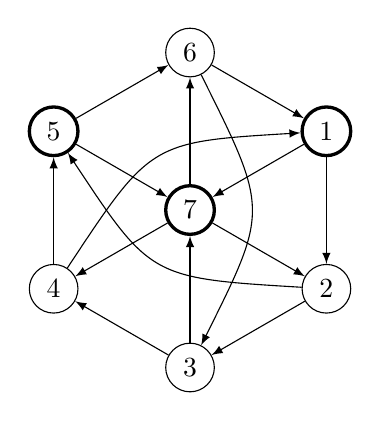
\begin{tikzpicture}
	\tikzstyle{every node}=[draw, shape = circle];
	
	\node[very thick] (1) at (90-60*1:2) {1};
	\node (2) at (90-60*2:2) {2};
	\node (3) at (90-60*3:2) {3};
	\node (4) at (90-60*4:2) {4};
	\node[very thick] (5) at (90-60*5:2) {5};
	\node (6) at (90-60*6:2) {6};
	\node[very thick] (7) at (0,0) {7};

	\draw[-latex] (1) -- (7);
	\draw[-latex] (3) -- (7);
	\draw[-latex] (5) -- (7);
	\draw[-latex] (7) -- (2);
	\draw[-latex] (7) -- (4);
	\draw[-latex] (7) -- (6);
	
	\draw[-latex] (1) -- (2);
	\draw[-latex] (2) -- (3);
	\draw[-latex] (3) -- (4);
	\draw[-latex] (4) -- (5);
	\draw[-latex] (5) -- (6);
	\draw[-latex] (6) -- (1);

	\draw[-latex] (2) .. controls(90-60*3.5:1) .. (5);
	\draw[-latex] (6) .. controls(90-60*1.5:1) .. (3);
	\draw[-latex] (4) .. controls(90-60*5.5:1) .. (1);
\end{tikzpicture}
\caption{%\ARCOMM{Yes: there are no graphs on $\leq 6$ vertices with this properties. I have checked that by case, using the fact that every tournament with $\nu=1$ has $\tau\leq 2$ [Bang-Jensen and S. Bessy, 2015].} 
The smallest graph with $\packing(D) = 1$ and $\tau(D) = 3$. A minimum feedback vertex set is highlighted.} \label{fig:nu=1_tau=3}
\end{figure}

The \BF{girth}\index{girth} of $D$ is the minimum length of a cycle in $D$, or by convention is infinity if $D$ is acyclic; we denote it as $\girth(D)$. Therefore, $\girth(D) = 1$ if and only if there is a loop on some vertex, $\girth(D) = 2$ if and only if there is no loop but there is an edge and $\girth(D) \ge 3$ if and only if $D$ is an oriented graph. We then have
$\girth(D) \packing(D) \le n$. The girth is related to the transversal number by $\gamma(D) \le n - \feedback(D) + 1$ and \cite{KLMR13}
\[
	(\girth(D) - 1) \feedback(D) \le 3 n \log_2 n \log_2 \log_2 n.
\]






A \BF{matching}\index{matching} is a set of disjoint edges; the \BF{matching number}\index{number!matching} of $D$, denoted as $\matching(D)$, is the maximum cardinality of a matching in $D$. If $D$ is a simple graph, then $\matching(D) = \packing(D)$ and $2 \matching(D) \ge \feedback(D)$. 

A simple graph is \BF{bipartite}\index{graph!bipartite} if its vertex set can be partitioned into $V = L \cup R$ and $L$ and $R$ are independent sets of $D$. Equivalently, a simple graph is bipartite if any of its cycles has even length. The K\"onig-Egerv\'ary theorem then asserts that if $D$ is bipartite, then $\matching(D) = \feedback(D)$. A \BF{tree}\index{tree} is a simple graph where all cycles have length two; clearly all trees are bipartite. A \BF{leaf}\index{leaf} is a vertex of in-degree one in a tree.


The \BF{clique}\index{clique} or \BF{complete graph}\index{graph!complete} on $n$ vertices $K_n$ is the simple graph with arc set $\{uv : u,v \in V, u \ne v\}$. A \BF{clique}\index{clique} in $D$ is any subgraph of $D$ isomorphic to $K_k$ for some $1 \le k \le n$. The \BF{clique number}\index{number!clique} of $D$, denoted as $\clique(D)$, is the maximum size of a clique in $D$. A \BF{clique cover}\index{clique cover} of $D$ is a set $H_1, \dots, H_t$ of cliques in $D$ such that $V(H_1) \cup \dots \cup V(H_t) = V$. The \BF{clique cover number}\index{clique cover number} of $D$ is the smallest number of parts in a clique cover of $D$ and is denoted by $\cliqueCover(D)$.



A \BF{$k$-colouring}\index{colouring} of a simple graph $D$ is a map $c : V \to \(k\)$ such that $c(u) \ne c(v)$ whenever $uv \in E$. The image $c(v)$ is referred to as the colour of $v$. Alternatively, a colouring can be viewed as a partition of $V$ into $k$ independent sets. The \BF{chromatic number}\index{number!chromatic} is the minimum number of colours used in any colouring of $D$; it is denoted by $\chromatic(D)$. Thus, $D$ is bipartite if and only if $\chromatic(D) = 2$. We then have
\[
	\chromatic(D) \ge \clique(D).
\]

The \BF{complement}\index{graph!complement of a} a simple graph $D = (V,E)$ is the simple graph $\bar{D} = (V, \{uv : u \ne v, uv \notin E\})$. Then $D$ is the complement of $\bar{D}$ and 
\begin{align*}
	\clique(D) &= \independence(\bar{D}),\\
	\cliqueCover(D) &= \chromatic(\bar{D}).
\end{align*}

A simple graph $D$ is a \BF{perfect graph} if $\chromatic(H) = \clique(H)$ for any induced subgraph $H$ of $D$. The strong perfect graph theorem \cite{CRST06} then asserts that $D$ is perfect if and only if it does not have any induced subgraph of the form $C_{2k+1}$ or $\overline{C_{2k+1}}$ for some $k \ge 2$ (i.e. no induced odd cycles and no induced complements of odd cycles). In particular, $D$ is perfect if and only if its complement $\bar{D}$ is perfect (this is the weak perfect graph theorem \cite{Lov72}).










\section{Signed graphs} \label{sec:signed_graphs}



We use the notation $\oplus$ and $\ominus$ to denote signs (which represent $1$ and $-1$, respectively). We then have the usual product of signs: $\oplus \cdot \oplus = \ominus \cdot \ominus = \oplus$ and $\oplus \cdot \ominus = \ominus \cdot \oplus = \ominus$; we further denote $\ominus = - \oplus$ and $\oplus = -\ominus$. A \BF{signed graph}\index{signed graph} with vertex set $V$ is a couple $G = (V,E)$, where $E\subseteq V^2\times\{\oplus , \ominus\}$ are the \BF{signed arcs} of $G$. If $(u,v,s) \in E$ we say that $G$ has an arc from $u$ to $v$ of sign $s$. Arcs are then called positive or negative as such:
\begin{alignat*}{2}
	E^\oplus	&:= \{uv : (u,v, \oplus) \in E\}	&\qquad& \textbf{positive arcs},\\
	E^\ominus 	&:= \{uv : (u,v, \ominus) \in E\}	&\qquad& \textbf{negative arcs}.
\end{alignat*}
Another classification of arcs is as follows:
\begin{alignat*}{2}
	E^0		&:= E^\oplus \cap E^\ominus 		&\qquad& \textbf{zero arcs},\\
	E^+		&:= E^\oplus \setminus E^\ominus	&\qquad& \textbf{strictly positive arcs},\\
	E^-		&:= E^\ominus \setminus E^\oplus	&\qquad& \textbf{strictly negative arcs},\\
	E^\pm	&:= E^+ \cup E^- 					&\qquad& \textbf{unate arcs}.
\end{alignat*}
We can then represent a signed graph in two different fashions: either the $\{\oplus, \ominus\}$-way, or the $\{ +, 0, - \}$-way. This is illustrated in Figure \ref{fig:signed_graphs}. The different neighbourhoods and degrees are defined accordingly, for instance the positive in-neighbourhood of $v$ is $\NInOplus(v) := \{u\in V:uv\in E^\oplus\}$.


\begin{figure}
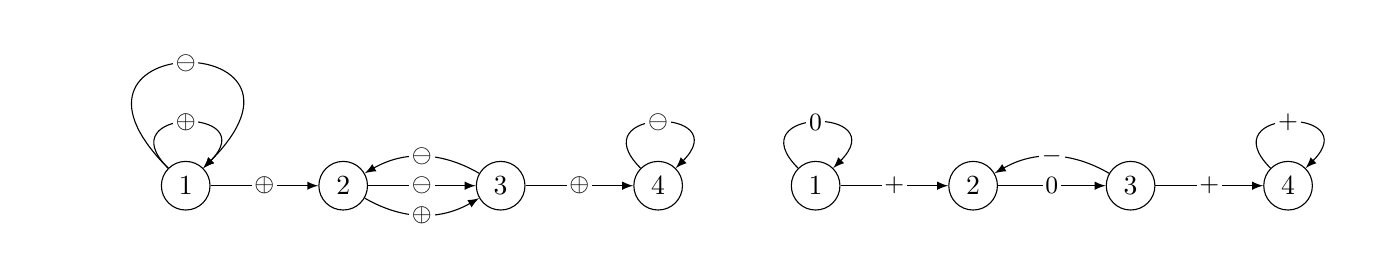
\begin{tikzpicture}[scale=2]
	\node[draw, shape = circle] (1) at (0,0) 	{$1$};
	\node[draw, shape = circle] (2) at (1,0) 	{$2$};
	\node[draw, shape = circle] (3) at (2,0) 	{$3$};
	\node[draw, shape = circle] (4) at (3,0) 	{$4$};

	\draw[-latex] (1) to node[midway,fill=white,inner sep=1] {\small $\oplus$}	(2);
	\draw[-latex] (2) to [bend right] node[midway,fill=white,inner sep=1] {\small $\oplus$}	(3);
	\draw[-latex] (2) to node[midway,fill=white,inner sep=1] {\small $\ominus$}	(3);
	\draw[-latex] (3) to [bend right] node[midway,fill=white,inner sep=1] {\small $\ominus$}	(2);
	\draw[-latex] (3) to node[midway,fill=white,inner sep=1] {\small $\oplus$}	(4);

	\draw[-latex] (1) .. controls(-0.5, 0.5) 	and (0.5, 0.5) 	.. (1) node[midway,fill=white,inner sep=1] {\small $\oplus$} 	(1);
	\draw[-latex] (1) .. controls(-1, 1) 	and (1, 1) 		.. (1) node[midway,fill=white,inner sep=1] {\small $\ominus$} 	(1);
	\draw[-latex] (4) .. controls(2.5, 0.5) 	and (3.5, 0.5) 	.. (4) node[midway,fill=white,inner sep=1] {\small $\ominus$} 	(4);

	\begin{scope}[xshift=4cm]
		\node[draw, shape = circle] (1) at (0,0) 	{$1$};
		\node[draw, shape = circle] (2) at (1,0) 	{$2$};
		\node[draw, shape = circle] (3) at (2,0) 	{$3$};
		\node[draw, shape = circle] (4) at (3,0) 	{$4$};
	
		\draw[-latex] (1) to node[midway,fill=white,inner sep=1] {\small $+$}	(2);
		\draw[-latex] (2) to node[midway,fill=white,inner sep=1] {\small $0$}	(3);
		\draw[-latex] (3) to [bend right] node[midway,fill=white,inner sep=1] {\small $-$}	(2);
		\draw[-latex] (3) to node[midway,fill=white,inner sep=1] {\small $+$}	(4);
	
		\draw[-latex] (1) .. controls(-0.5, 0.5) 	and (0.5, 0.5) 	.. (1) node[midway,fill=white,inner sep=1] {\small $0$} 	(1);
		\draw[-latex] (4) .. controls(2.5, 0.5) 	and (3.5, 0.5) 	.. (4) node[midway,fill=white,inner sep=1] {\small $+$} 	(4);
	\end{scope}
\end{tikzpicture}
\caption{Two ways of representing the same signed graph} \label{fig:signed_graphs}
\end{figure}




We say $G$ is \BF{positive} if all its arcs are positive, i.e. $E^\ominus = \emptyset$, \BF{negative} if $E^\oplus = \emptyset$, \BF{unate} if $E^0 = \emptyset$ and \BF{zero} if $E^\pm = \emptyset$. 

A \BF{subgraph}\index{subgraph} of $G$ is $G' = (V',E')$, where $V' \subseteq V$ and $E' \subseteq E \cap \left( (V')^2 \times \{\oplus, \ominus\} \right)$; we denote $G' \subseteq G$. An \BF{induced subgraph}\index{subgraph!induced} of $G$ is obtained by removing vertices of $G$, i.e. $G'$ is and induced subgraph of $G$ if $V' \subseteq V$ and $E' = E \cap \left( (V')^2 \times \{\oplus, \ominus\} \right)$. If $I \subseteq V$, we denote by $G[I]$ the subgraph of $G$ induced by $I$ and we set $G \setminus I = G[V\setminus I]$.  When the context is clear, we shall identify an induced subgraph with its vertex set. A \BF{spanning subgraph}\index{subgraph!spanning} of $G$ is obtained by removing arcs, i.e. $G'$ is a spanning subgraph of $G$ if $V' = V$ and $E' \subseteq E$.


%The \BF{positive}, \BF{negative}, \BF{unate} and \BF{zero in-neighbourhoods}\index{neighborhood!positive}\index{neighborhood!negative}\index{neighborhood!unate}\index{neighborhood!zero} of $v$ are defined accordingly, 
%\begin{align*}
%,\\
%\NInMinus(v;G) &:= \{u\in V:uv\in E^-\},\\ 
%\NInZero(v;G) &:= \{u\in V:uv\in E^0\},\\
%\NInPM(v;G) &:=\{u\in V:uv\in E^\pm\}.
%\end{align*} 
%The \BF{positive}, \BF{negative}, \BF{unate} and \BF{zero} \BF{out-neighbourhoods}, \BF{in-degrees}, and \BF{out-degrees} are defined similarly.\index{degree!positive}\index{degree!negative}\index{degree!unate}\index{degree!zero} When $G$ is clear from the context, we often omit it in the notation, and write $\NInPlus(v)$ instead of $\NInPlus(v;G)$ for example. The notion of minimum, maximum and average degree of a vertex are extend to signed graphs in the natural way. For instance, $\dInMinPlus(G):=\min_{v\in V}\dInPlus(v)$.  

The \BF{underlying graph}\index{unsigned version}\index{graph!underlying} of $G$ is the graph $|G|:=(V, E^\oplus \cup E^\ominus)$. Conversely, if $D$ is a graph and $\sigma : E(D) \to \{-1,0,1\}$ is an arc labelling function, then $(D,\sigma)$ is the signed graph with the same vertex set as $D$ such that
\begin{align*}
	E^\oplus (D,\sigma)		&:=\{uv\in E(D): \sigma(uv)\geq 0\},\\
	E^\ominus (D,\sigma)	&:=\{uv\in E(D): \sigma(uv)\leq 0\}.
\end{align*}
All the notions that do not involve signs apply on $G$ or $|G|$ indifferently. For instance, the packing number of $G$ equals the one of $|G|$, and we write $\packing(G)=\packing(|G|)$. Given a graph $D$,  we denote by $D^+$ the signed graph $(D,\sigma)$ where $\sigma=\cst=1$; $D^-$ and $D^0$ are defined similarly. A \BF{signed path} (resp. \BF{signed cycle}) is a unate signed graph $G$ whose underlying graph is a path (resp. cycle). We say that $G$ is \BF{balanced}\index{graph!balanced} if it has no negative cycles. 

A walk in $G$ of length $k$ is a sequence $v_0s_0v_1s_1\dots s_{k-1}v_k$ such that $(v_i,v_{i+1},s_i)\in E$ for all $0\leq i\leq k-1$. The \BF{sign of a walk} is the product of the sign of its arcs. A positive (resp. negative) path from $u$ to $v$ in $G$ can then be viewed as a positive (resp. negative) walk in $G$ beginning in $u$ and ending at $v$ such that all the vertices on the walk are distinct. A positive (resp. negative) cycle in $G$ can also be viewed as a positive (resp. negative) walk in $G$ of the form $v_0,s_0 v_1, \dots, v_{k-1},s_{k-1}, v_k = v_0$ and $v_i \ne v_j$ are distinct for all $0 \le i < j \le k-1$. A positive (resp. negative) loop $uu$ of $G$ then corresponds to a positive (resp. negative) cycle of length $1$. A \BF{chord}\index{chord} in a cycle $v_0,s_0 v_1, \dots,s_{k-1}, v_{k-1}$ is an arc $(v_i,v_j,s) \in E$ distinct from $(v_i,v_{i+1},s_i)$. A cycle is \BF{chordless}\index{cycle!chordless} if it has no chord.

A \BF{positive feedback vertex set}\index{set!feedback vertex}, is a subset $I \subseteq V$ such that $G\setminus I$ has no positive cycles \MGCOMM{A name for that property?}. The \BF{positive transversal number}\index{number!transversal} of $G$ is the size of a minimum positive (resp. negative) feedback vertex set of $G$ and is denoted by $\feedbackPlus(G)$. The \BF{negative feedback vertex sets} of $G$ and the \BF{negative transversal number} of $G$, denoted as $\feedbackMinus(G)$, are defined similarly. The \BF{positive packing number}\index{number!packing} of $G$, denoted as $\packingPlus(G)$, is the maximum number of vertex-disjoint positive cycles in $G$. The \BF{positive girth}\index{girth} of $G$ is the minimum length of a positive cycle in $G$, or by convention is infinity if $G$ has no positive cycles; we denote it as $\girthPlus(G)$. The \BF{negative packing number} $\packingMinus(G)$ and \BF{negative girth} $\girthMinus(G)$ are defined similarly. We have 
\begin{align*}
\girthPlus(G)\packingPlus(G)&\leq n,\\
\girthMinus(G)\packingMinus(G)&\leq n,\\
\girthPlus(G)&\leq n-\feedbackPlus(G)+1,\\
\girthMinus(G)&\leq n-\feedbackMinus(G)+1.
\end{align*}
%\ARCOMM{Maybe I could explain that there is no function $\phi^+$ such that $\feedbackPlus(G)\leq\phi^+(\packingPlus(G))$ neither $\phi^-$ such that  $\feedbackPlus(G)\leq\phi^+(\packingPlus(G))$.} 

Given $I\subseteq V$, the \BF{$I$-switch}\index{switch} of $G=(V,E)$ is the signed graph $G'=(V',E')$ obtained from $G$ by switching the sign of every arc with one end in $I$ and the other outside $I$, that is:
\[
	E'=\{(u,v,s):(u,v,s)\in E\text{ and }|\{u,v\}\cap I|\neq 1,\text{ or }(u,v,-s)\in E\text{ and }|\{u,v\}\cap I|= 1\} 
\]
Two signed graphs $G$ and $G'$ are \BF{switch-equivalent} if $G'$ is the $I$-switch of $G$ for some $I$. Many important features are preserved by the switch operation. For instance, $\girthPlus$, $\girthMinus$, $\feedbackPlus$, $\feedbackMinus$, $\packingPlus$, and $\packingMinus$ are invariant for this operation. The \BF{frustration index} $\lambda(G)$ is the minimum number of negative arcs in a switch of $G$; equivalently $\lambda(G)$ is equal to the minimum number of arcs to remove in $G$ order to obtain a balanced signed graph. Hence, $\lambda(G)=0$ if and only if $G$ is balanced. 

%Synonym for frustration index: index of imbalance







\section{Logical connectives} \label{sec:logical_connectives}

We now review some basic facts about the main logical connectives. Let $a, b \in \{0,1\}$, the \BF{negation}\index{negation} of $a$, the \BF{conjunction}\index{conjunction} of $a$ and $b$ and the \BF{disjunction}\index{disjunction} of $a$ and $b$ are respectively defined as
\begin{align*}
	\neg a &= \begin{cases}
		1 &\text{if } a = 0,\\
		0 &\text{if } a = 1,
	\end{cases}
	\\
	a \land b &= \begin{cases}
		1 &\text{if } a = 1 \text{ and } b = 1\\
		0 &\text{otherwise},
	\end{cases}
	\\
	a \lor b &= \begin{cases}
		1 &\text{if } a = 1 \text{ or } b = 1\\
		0 &\text{otherwise}.
	\end{cases}
\end{align*}
Equivalently, $\neg a = 1 - a$, $a \land b = \min \{a, b\}$ and $a \lor b = \max \{a, b \}$. Since conjunction and disjunction are commutative (i.e. $a \land b = b \land a$ and $a \lor b  = b \lor a$) and associative (i.e. $a \land (b \land c) = (a \land b) \land c$ and similarly for disjunction), we can define $\bigwedge_{i=1}^k a_i$ and $\bigvee_{i=1}^k a_k$ for $a_1, \dots, a_k \in \{0,1\}$. By convention, an empty conjunction is equal to $1$ while an empty disjunction is $0$.

Some basic properties of these three logical connectives are listed below, where $a,b,c \in \{0,1\}$
\begin{align*}
	\neg \neg a &= a,\\
	a \land (b \lor c) &= (a \land b) \lor (a \land c),\\
	a \lor (b \land c) &= (a \lor b) \land (a \lor c),\\
	\neg (a \land b) &= \neg a \lor \neg b,\\
	\neg (a \lor b) &= \neg a \land \neg b.
\end{align*}
Any Boolean function $\phi : \{0,1\}^n \to \{0,1\}$ can be expressed using $\land, \lor, \neg$ (see Exercise \ref{exerc:dnf}).

Moreover, for any property $\mathcal{P}$, we denote the function which returns $1$ if $\mathcal{P}$ is satisfied and $0$ otherwise by $\one{\mathcal{P}}$. For instance, $a \land b = \one{ (a,b) = (1,1) }$.




\section{Permutation groups and transformation semigroups} \label{sec:algebraic_background}

A binary operation $*$ on a set $S$ is simply a function $* : S^2 \to S$ and we write $a * b$ instead of $*(a,b)$. The operation is associative if $a * (b * c) = (a * b) * c$ for all $a,b,c \in S$. A pair $(S,*)$, where $*$ is associative is called a \BF{semigroup}\index{semigroup}. An element $e \in S$ is called the \BF{identity}\index{identity} if $e * a = a * e = a$ for all $a \in S$. A semigroup with identity is a \BF{monoid}\index{monoid}. A \BF{group}\index{group} is a monoid in which every element $a$ has a unique inverse $a^{-1}$ such that $a * a^{-1} = a^{-1} * a = e$. A group is \BF{abelian}\index{group!abelian} if its operation is commutative, i.e. $a * b = b * a$ for all $a,b \in S$.

\begin{example}\label{ex:semigroups}
\begin{enumerate}
	\item The following are semigroups:
	\begin{itemize}
		\item $(S, *)$ where $a * b = a$ for all $a,b \in S$;
		
		\item $(\{0,2,4,\dots\}, \times)$;
		
		\item the set $\Sing(n)$ of all non-surjective functions $\phi : \{1, \dots, n\} \to \{1, \dots, n\}$, equipped with composition.
	\end{itemize}
	 
	\item The following are monoids:
	\begin{itemize}
		\item $(2^T, \cup)$, where $T$ is any set and $2^V$ is its power set;

		\item the conjunction $(\{0,1\}, \land)$ and the disjunction $(\{ 0,1 \}, \lor)$;
			
		\item more generally, $(\{0,1,\dots, q-1\}, \min)$ and $(\{0,1,\dots, q-1\}, \max)$;
		
		\item $(\mathbb{N}, +)$.
	\end{itemize}

	\item The following are abelian groups:
	\begin{itemize}
		\item $(\mathbb{Z}, +)$;
	
		\item $(\mathbb{Q} \setminus \{0\}, \times)$;
	
		\item $(\mathbb{R} \setminus \{0\}, \times)$.
	\end{itemize}
\end{enumerate}
\end{example}

Let $B$ be a finite set and let $f : B \to B$. Such a function $f$ is commonly referred to as a \BF{transformation}\index{transformation} of $B$. The set of all transformations of $B$, endowed with composition, forms the \BF{full transformation semigroup}\index{semigroup!full transformation} $\Tran(B)$ of $B$. If $f$ is bijective (or equivalently, injective; or equivalently, surjective), we say that $f$ is a \BF{permutation}\index{permutation} of $B$. The set of all permutations of $B$, endowed with composition, forms the \BF{symmetric group}\index{group!symmetric} $\Sym(B)$ of $B$. Moreover, $f$ is \BF{singular}\index{transformation!singular} if $f$ is not a permutation of $B$. Then $\Sing(B) = \Tran(B) \setminus \Sym(B)$ is the \BF{singular semigroup}\index{semigroup!singular} of $B$.

A subsemigroup $S'$ of $S$ is a subset of $S$ which is itself a semigroup; we denote $S' \le S$. For any semigroup $S$ and any $T \subseteq S$, the subsemigroup generated by $T$, denoted by $\langle T \rangle$, is the set of all elements of $S$ which can be expressed as a product of elements of $T$. Equivalently, $\langle T \rangle$ is the intersection of all the subsemigroups of $S$ containing $T$. If $\langle T \rangle = S$, we say that $T$ is a \BF{generating set}\index{set!generating} for $S$. There are many classical generating sets for the symmetric group $\Sym(B)$ (see Exercise \ref{exerc:generating_sets_symmetric_group}); one of them is the set of all transpositions. Let $a \ne b \in B$, then the \BF{transposition}\index{transposition} of $a$ and $b$, denoted as $(a \ b)$, works as you might expect:
\[
	(a \espace b)(x) = \begin{cases}
	b &\text{if } x = a,\\
	a &\text{if } x = b,\\
	x &\text{otherwise.}
	\end{cases}
\]
The semigroup $\Sing(B)$ of singular transformations of $B$ has a similar generating set. For $a \ne b \in B$, the \BF{assignment}\index{assignment} of $a$ to $b$, denoted as $(a \to b)$ is defined by:
\[
	(a \to b) (x) = \begin{cases}
	b &\text{if } x = a,\\
	x &\text{otherwise.}
	\end{cases}
\]
Then the set of all assignments of $B$ is a generating set of $\Sing(B)$. The \BF{rank} of a transformation is the number of its images. Finally, Exercise \ref{exerc:generating_sets_tran} asks you to prove the following fundamental result: if $f$ is a transformation of $B$ with rank $|B|-1$, then $\Sym(B) \cup f$ is a generating set of $\Tran(B)$.

For any $f \in \Tran(B)$ and $g \in \Sym(B)$, the \BF{conjugation}\index{conjugation} of $f$ by $g$ is 
\[
	f^g := g \circ f \circ g^{-1} \in \Tran(B).
\]
Conjugation is very important, as $f^g$ acts like $f$, up to renaming the elements of $B$ by $g$. As such, conjugation preserves many properties of the transformation $f$.

Every permutation $g \in \Sym(B)$ can be expressed using its cycle expansion
\[
	g = (b_1 \espace g(b_1) \espace \cdots \espace g^{-1}(b_1)) (b_2 \espace g(b_2) \espace \cdots \espace g^{-1}(b_2)) \cdots (b_k \espace g(b_k) \espace \cdots \espace g^{-1}(b_k)),
\]
where fixed points are usually omitted from this representation. We then say that $b_i, g(b_i), \dots, g^{-1}(b_i)$ is a cycle of $g$. As mentioned above, any permutation can be expressed as a composition of transpositions. In fact, either $g$ can be expressed as a composition of an even number of transpositions, or as a composition of an odd number of transpositions. We then refer to $g$ as \BF{even}\index{permutation!even} or \BF{odd}\index{permutation!odd} (there are as many odd as even permutations of $B$ if $|B| \ge 2$). A permutation $g$ is even if and only if $g$ contains an even number of cycles of even length. The even permutations of $B$ form the \BF{alternating group}\index{group!alternating} of $B$, denoted as $\Alt(B)$.

As an illustration, the permutations in $\Sym(\{1,2,3,4\})$ are given with their respective cycle expansion in Table \ref{table:Sym4}.

\begin{table}
\centering
\begin{tabular}{|l|l|l|}
	\hline
	$g(1)g(2)g(3)g(4)$ 	& Cycle expansion 					& Parity\\
	\hline
	1234				& (1)								& Even\\
	1243				& (3 \espace 4)						& Odd\\
	1324				& (2 \espace 3)						& Odd\\
	1342				& (2 \espace 3 \espace 4)			& Even\\
	1423				& (2 \espace 4 \espace 3)			& Even\\
	1432				& (2 \espace 4)						& Odd\\
	2134				& (1 \espace 2)						& Odd\\
	2143				& (1 \espace 2) (3 \espace 4)		& Even\\
	2314				& (1 \espace 3 \espace 2)			& Even\\
	2341				& (1 \espace 4 \espace 3 \espace 2)	& Odd\\
	2413				& (1 \espace 2 \espace 4 \espace 3)	& Odd\\
	2431				& (1 \espace 2 \espace 4)			& Even\\
	3124				& (1 \espace 3 \espace 2)			& Even\\
	3142				& (1 \espace 3 \espace 4 \espace 2)	& Odd\\
	3214				& (1 \espace 3)						& Odd\\
	3241				& (1 \espace 3 \espace 4)			& Even\\
	3412				& (1 \espace 3) (2 \espace 4)		& Even\\
	3421				& (1 \espace 3 \espace 2 \espace 4)	& Odd\\
	4123				& (1 \espace 4 \espace 3 \espace 2)	& Odd\\
	4132				& (1 \espace 4 \espace 2)			& Even\\
	4213				& (1 \espace 4 \espace 3)			& Even\\
	4231				& (1 \espace 4)						& Odd\\
	4312				& (1 \espace 4 \espace 2 \espace 3)	& Odd\\
	4321				& (1 \espace 4) (2 \espace 3)		& Even\\
	\hline
\end{tabular}
\caption{The permutations in $\Sym(\{1, \dots, 4\})$} \label{table:Sym4}
\end{table}


An \BF{automorphism}\index{graph automorphism} of a graph $D$ is an isomorphism to itself, i.e. it is any permutation $\phi$ of its vertex set such that $uv \in E$ if and only if $\phi(u)\phi(v) \in E$. The set of all automorphisms forms the \BF{automorphism group}\index{group!automorphism} $\Aut(D)$ of $D$. A graph is \BF{vertex-transitive}\index{graph!vertex-transitive} if its automorphism group acts transitively on its vertex set, i.e. if for all $u,v \in V$, there exists $\phi \in \Aut(D)$ such that $\phi(u) = v$.




\section{Finite fields} \label{sec:GF}


A \BF{field}\index{field} is an algebraic structure in which we can add, subtract, multiply and divide (and where multiplication distributes over addition), just like over the real numbers. Formally, $(F,+,\times,0,1)$ is a field if $(F,+,0)$ and $(F \setminus\{0\},\times,1)$ are abelian groups (with the corresponding identity elements) and if $a \times (b + c) = (a \times b) + (a \times c)$ for all $a,b,c, \in F$. 

Any \BF{finite field}\index{field!finite} is of order (size) $q = p^m$, where $p$ is a prime number and $m$ is any integer $\ge 1$. Moreover, all fields of order $q$ are isomorphic. We can then talk about the field of order $q$, commonly denoted as $\GF(q)$ (for Galois field, in honour of Evariste Galois)\index{field!Galois}. 

The finite fields are constructed as follows. First of all, $\GF(p)$ corresponds to arithmetic modulo $p$. 

\begin{example}[The binary field $\GF(2)$]
The smallest, and arguably simplest, field is $\GF(2)$, whose addition and multiplication table are displayed in Figure \ref{fig:GF2}. We can then compare logical operations and binary field operations as such:
\begin{align*}
	x \land y	&= xy\\
	x \lor y 	&= x + y + xy\\
	(x \land \neg y) \lor (\neg x \land y) &= x + y\\
	\neg x 		&= x + 1.
\end{align*}
\end{example}


\begin{figure}
\centering
\begin{tabular}{c|ccc}
	$+$ & $0$ & $1$\\
	\hline
	$0$ & $0$ & $1$\\
	$1$ & $1$ & $0$
\end{tabular} \hspace{2cm}
\begin{tabular}{c|ccccc}
	$\times$ & $0$ & $1$\\
	\hline
	$0$ & $0$ & $0$\\ 
	$1$ & $0$ & $1$
\end{tabular}
\caption{The addition and multiplication tables of $\GF(2)$} \label{fig:GF2}
\end{figure}


\begin{example}[$\GF(5)$]
The tables of arithmetic modulo $5$ are easy to determine and given in Figure \ref{fig:GF5}. When working modulo $5$, we can add, subtract, multiply and divide (not by zero, of course): 
\begin{alignat*}{4}
	-1 &= 4, 		&\qquad -2 &= 3,		&\qquad -3 &= 2, 	&\qquad -4 &= 1,\\
	1^{-1} &= 1, 	&\qquad 2^{-1} &= 3, &\qquad 3^{-1} &= 2, &\qquad 4^{-1} &= 4.
\end{alignat*}
\end{example}


\begin{figure}
\centering
\begin{tabular}{c|ccccc}
	$+$ & $0$ & $1$ & $2$ & $3$ & $4$\\
	\hline
	$0$ & $0$ & $1$ & $2$ & $3$ & $4$\\
	$1$ & $1$ & $2$ & $3$ & $4$ & $0$\\
	$2$ & $2$ & $3$ & $4$ & $0$ & $1$\\
	$3$ & $3$ & $4$ & $0$ & $1$ & $2$\\
	$4$ & $4$ & $0$ & $1$ & $2$ & $3$
\end{tabular} \hspace{2cm}
\begin{tabular}{c|ccccc}
	$\times$ & $0$ & $1$ & $2$ & $3$ & $4$\\
	\hline
	$0$ & $0$ & $0$ & $0$ & $0$ & $0$\\
	$1$ & $0$ & $1$ & $2$ & $3$ & $4$\\
	$2$ & $0$ & $2$ & $4$ & $1$ & $3$\\
	$3$ & $0$ & $3$ & $1$ & $4$ & $2$\\
	$4$ & $0$ & $4$ & $3$ & $2$ & $1$
\end{tabular}
\caption{The addition and multiplication tables of $\GF(5)$} \label{fig:GF5}
\end{figure}



To construct $\GF(p^m)$ in general, let $P(x)$ be a polynomial of degree $m$ over $\GF(p)$. $P(x)$ is \BF{irreducible}\index{polynomial!irreducible} if it cannot be factored as $P(x) = Q(x)R(x)$ with $\deg Q(x), \deg R(x) < m$. Moreover, $P(x)$ is \BF{primitive}\index{polynomial!irreducible} if it is irreducible and the smallest positive integer $n$ such that $P(x) \mid x^n - 1$ is $n = p^m-1$. It can be shown that a primitive polynomial of degree $m$ over $\GF(p)$ exists for all $p$ and $m$. Let $P(x)$ be such a polynomial, and let $\alpha$ be one of its roots. Then $\GF(p^m) = \{0,1,\alpha,\dots, \alpha^{p^m-2}\}$.

\begin{example}[Construction of $\GF(4)$]
Let $\alpha$ be a root of $x^2 + x + 1$, and let us construct $\GF(4)$. We have the following relations:
\begin{align*}
%	\alpha + \alpha &= \alpha (1 + 1) = \alpha \cdot 0 = 0,\\
	a + a &= a(1 + 1) = a \cdot 0 = 0, \quad \forall\ a \in \GF(4),\\
	\alpha^2 &= \alpha + 1,\\
	\alpha^3 &= \alpha^2 \cdot \alpha = (\alpha + 1) \alpha = \alpha^2 + \alpha = 1.
\end{align*}
Then the addition and multiplication tables of $\GF(4)$ are given in Figure \ref{fig:GF4}.

\begin{figure}
\centering
\begin{tabular}{c|c|c|c|c|}
	$+$ & $0$ & $1$ & $\alpha$ & $\alpha+1$\\
	\hline
	$0$ & $0$ & $1$ & $\alpha$ & $\alpha+1$\\
	\hline
	$1$ & $1$ & $0$ & $\alpha+1$ & $\alpha$\\
	\hline
	$\alpha$ & $\alpha$ & $\alpha+1$ & $0$ & $1$\\
	\hline
	$\alpha+1$ & $\alpha+1$ & $\alpha$ & $1$ & $0$\\
	\hline
\end{tabular} \hspace{2cm}
\begin{tabular}{c|c|c|c|c|}
	$\times$ & $0$ & $1$ & $\alpha$ & $\alpha^2$\\
	\hline
	$0$ & $0$ & $0$ & $0$ & $0$\\
	\hline
	$1$ & $0$ & $1$ & $\alpha$ & $\alpha^2$\\
	\hline
	$\alpha$ & $0$ & $\alpha$ & $\alpha^2$ & $1$\\
	\hline
	$\alpha^2$ & $0$ & $\alpha^2$ & $1$ & $\alpha$\\
	\hline
\end{tabular}
\caption{The addition and multiplication tables of $\GF(4)$} \label{fig:GF4}
\end{figure}

\end{example}


The multiplicative structure $\GF(q)^* = \GF(q) \setminus \{0\}$ is very simple: it is that of a cyclic group of order $q-1$, i.e. $\GF(q)^* = \{\alpha, \alpha^2, \dots, \alpha^{q-2}, \alpha^{q-1} = 1\}$, where $\alpha$ is the root of $P(x)$. This is the \BF{exponential notation}\index{exponential notation}. For the additive structure, for any $\beta \in \GF(p^m)$, we have $p \beta = \beta + \beta + \dots + \beta = 0.$ We say that $p$ is the \BF{characteristic}\index{characteristic} of $\GF(p^m)$. More generally, $\GF(p^m)$ forms a vector space of dimension $m$ over $\GF(p)$, with the polynomial basis $1, \alpha, \dots, \alpha^{m-1}$. This yields the \BF{polynomial notation}\index{polynomial notation}:
\[
	\beta = \sum_{i=0}^{m-1} \beta_i \alpha^i \quad \beta_i \in \GF(p).
\]

\begin{example}[Exponential-polynomial conversion for $\GF(8)$]
Let $\alpha$ be a root of $x^3 + x + 1$, i.e. 
\[
	\alpha^3 + \alpha + 1 = 0.
\]
Then $\GF(8) = \{0,1,\alpha,\alpha^2,\alpha^3  = \alpha+1, \alpha^4 = \alpha^2 + \alpha, \alpha^5 = \alpha^2 + \alpha + 1, \alpha^6 = \alpha^2 + 1\}.$
\end{example}


A major feature of finite fields is that any function $\phi: \GF(q) \to \GF(q)$ is a polynomial, i.e. there exist $\phi_0, \dots, \phi_{q-1} \in \GF(q)$ such that 
\[
	\phi(a) = \sum_{d=0}^{q-1} \phi_d a^d
\]
and this representation is unique. This feature can be extended to multivariate functions.



Let $\GF(q)^{n \times n}$ be the set of all $n \times n$ matrices over $\GF(q)$. This set, endowed with multiplication, forms the \BF{general linear semigroup}\index{semigroup!general linear} $\GLS(n,q)$ of $\GF(q)^n$. Viewing a matrix ${\bf M} \in \GLS(n,q)$ as the transformation $f \in \Tran(\GF(q)^n)$, where $f(x) = x{\bf M}$, we can naturally embed $\GLS(n,q)$ as a subsemigroup of $\Tran(\GF(q)^n)$. The set of all nonsingular matrices in $\GLS(n,q)$ forms the \BF{general linear group}\index{group!general linear} $\GL(n,q)$ of $\GF(q)^n$.


\section{The state space} \label{sec:state_space}


We shall usually consider $\(q\) := \{0, 1, \dots, q-1\}$ endowed with an abelian group structure (for instance, addition modulo $q$); if $q$ is a prime power, we will also view $\(q\)$ as the finite field $\GF(q)$. Let $[n] = \{1, \dots, n\}$, then a \BF{state}\index{state} is any $x = (x_1, \dots, x_n) \in \(q\)^n$.

We shall use the following shorthand notation: for any $S = \{s_1, \dots, s_k\} \subseteq [n]$, we denote $x_S = (x_{s_1}, \dots, x_{s_k})$, where the order is irrelevant unless specified. The $v$-th \BF{unit state}\index{state!unit} is given by $e^v = (0,\dots,0,1,0,\dots,0)$, where $e^v_v = 1$. We shall abbreviate the \BF{all-zero state}\index{state!all-zero} $(0,\dots,0)$ to $0$ when the context is clear; we use similar notation for the \BF{all-one state}\index{state!all-one} $(1,\dots,1)$ or any other state of the form $(a, \dots, a)$ for some $a \in \(q\)$.

We also endow $\(q\) = \{0, \dots, q-1\}$ with the natural order $0 < 1< \dots q-1$. By extension, for any $x,y \in \(q\)^n$, we write $x \le y$ if $x_v \le y_v$ for all $v \in [n]$. The state space $\(q\)^n$ endowed with that partial order forms a distributive lattice (see for example the authoritative book \cite{Gra13} for more details). It is illustrated for $\(2\)^3$ and $\(3\)^2$ in Figure \ref{fig:Hasse} by its Hasse diagram, the simple graph where $xy$ is an edge if and only if $x \le y$ and there is no $z$ with $x < z < y$.

\begin{figure}
\centering
\subfloat[$\{0,1\}^3$]{
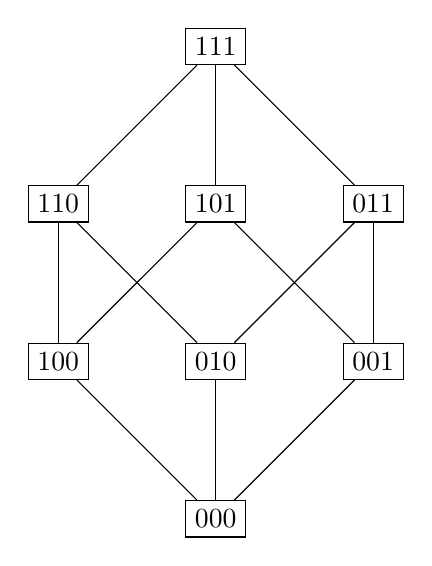
\begin{tikzpicture}[scale=2]
	\node[draw]	(000) at (1,0) {$000$};
	\node[draw]	(001) at (2,1) {$001$};
	\node[draw]	(010) at (1,1) {$010$};
	\node[draw]	(011) at (2,2) {$011$};
	\node[draw]	(100) at (0,1) {$100$};
	\node[draw]	(101) at (1,2) {$101$};
	\node[draw]	(110) at (0,2) {$110$};
	\node[draw]	(111) at (1,3) {$111$};

	\draw	(000) -- (100);
	\draw	(000) -- (010);
	\draw	(000) -- (001);


	\draw	(100) -- (110);
	\draw	(100) -- (101);
	\draw	(010) -- (110);
	\draw	(010) -- (011);
	\draw	(001) -- (101);
	\draw	(001) -- (011);

	\draw	(111) -- (110);
	\draw	(111) -- (101);
	\draw	(111) -- (011);
\end{tikzpicture}
}\hspace{2cm}%
\subfloat[$\{0,1,2\}^2$]{
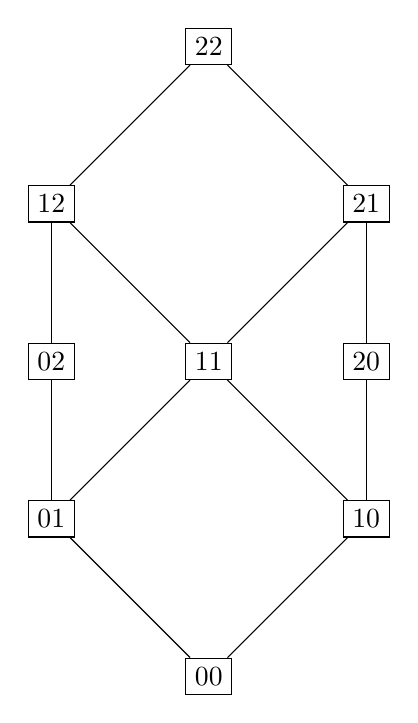
\begin{tikzpicture}[scale=2]
	\node[draw]	(00) at (1,0) {$00$};
	\node[draw]	(01) at (0,1) {$01$};
	\node[draw]	(10) at (2,1) {$10$};
	\node[draw]	(11) at (1,2) {$11$};
	\node[draw]	(02) at (0,2) {$02$};
	\node[draw]	(20) at (2,2) {$20$};
	\node[draw]	(12) at (0,3) {$12$};
	\node[draw]	(21) at (2,3) {$21$};
	\node[draw]	(22) at (1,4) {$22$};

	\draw	(00) -- (10);
	\draw	(00) -- (01);

	\draw	(10) -- (20);
	\draw	(10) -- (11);

	\draw	(01) -- (11);
	\draw	(01) -- (02);

	\draw	(11) -- (21);
	\draw	(11) -- (12);

	\draw	(20) -- (21);
	\draw	(02) -- (12);

	\draw	(21) -- (22);
	\draw	(12) -- (22);
\end{tikzpicture}
}
\caption{The lattice of some state spaces.} \label{fig:Hasse}
\end{figure}



We say that two states $a$ and $b$ are \BF{comparable}\index{states!comparable} if either $a \le b$ or $b \le a$; they are \BF{incomparable} otherwise. For any $x \le y$, we define the \BF{interval}\index{interval} $[x,y]$ as any state comparable to both $x$ and $y$: $[x,y] := \{z \in \(q\)^n : x \le z \le y \}$.

A \BF{chain}\index{chain} of length $k$ is a sequence of distinct, mutually comparable states: $x^0, \dots, x^k$ such that $x^i \le x^{i+1}$ for all $0 \le i \le k-1$. Clearly, the longest chain in $\(q\)^n$ has length $n(q-1)$.

Conversely, an \BF{antichain}\index{antichain} is a set of mutually incomparable states: $y^1, \dots, y^l$ such that $y^i \not\le y^j$ for all distinct $1 \le i,j \le l$. Sperner's theorem states that the largest antichain in $\(2\)^n$ is the layer of states with exactly $\lfloor n/2 \rfloor$ ones. We shall use this theorem, along with some of its generalisations, in Chapter \ref{ch:guessing_number_signed}.



\section{Hamming and Manhattan metrics} \label{sec:Hamming_metric}


The \BF{Hamming distance}\index{distance!Hamming} between $x, y \in \(q\)^n$ is the number of coordinates where they differ:
\begin{align*}
	\Delta(x,y) &= \{v \in [n]: x_v \ne y_v\},\\
	\dH(x,y) &= |\Delta(x,y)|.
\end{align*}
The \BF{Hamming weight}\index{weight!Hamming} of $x$ is the number of non-zero coordinates in $x$:
\[
	\wH(x,y) = |\{v \in [n]: x_v \ne 0\}|= \dH(x, 0).
\]

The \BF{Hamming graph}\index{graph!Hamming} $H(n,q)$ is the simple graph with vertex set $\(q\)^n$, where two vertices are adjacent if and only if they are at Hamming distance one. The \BF{$n$-hypercube}\index{hypercube} is the Hamming graph $Q_n := H(n,2)$. We have 
\begin{align*}
	d(H(n,q)) &= n (q-1),\\
	\clique(H(n,q)) &= q,\\
	\independence(H(n,q)) &= q^{n-1}.
\end{align*}

The automorphism group of the Hamming graph is given by all the permutations $\phi$ of $\(q\)^n$ of the form
\[
	\phi(x) = (\psi^1(x_{\pi(1)}), \dots, \psi^n(x_{\pi(n)}) ),
\]
for some $\pi \in \Sym([n])$ and some family $\psi^1, \dots, \psi^n \in \Sym(\(q\))$. In particular, the Hamming graph is vertex-transitive. This automorphism group coincides with the isometry group of the Hamming metric, i.e. 
\[
	\phi \in \Aut(H(n,q)) \iff \dH(\phi(x), \phi(y)) = \dH(x, y) \quad \forall x,y \in \(q\)^n.
\]


An \BF{$(n,q)$-Gray code}\index{Gray code} is an enumeration of $\(q\)^n$, say $G = (x^1, \dots, x^{q^n})$ such that $\dH(x^i, x^{i+1}) = 1$ for all $1 \le i \le q^n - 1$. Moreover, if $\dH(x^{q^n}, x^1) = 1$, the Gray code is called \BF{cyclic}\index{Gray code!cyclic}. Cyclic Gray codes exist for all values of $n$ and $q$. For instance, there is a natural recursive construction for $q=2$. For $n=1$, $G_1 = (0,1)$; then $G_{n+1}$ is obtained by adding a zero in front of $G_n$, and then by adding a one in front of $G_n$ in reverse. This may sound a bit confusing, but hopefully the first few $G_n$s will help:
\[
	G_1 = \begin{array}{|l|}
	\hline
	0 \\
	1 \\
	\hline
	\end{array},
	\quad 
	G_2 = \begin{array}{|l|l|}
	\hline
	0 & 0 \\
	0 & 1 \\
	\hline
	1 & 1 \\
	1 & 0 \\
	\hline
	\end{array},
	\quad
	G_3 = \begin{array}{|l|ll|}
	\hline
	0 & 0 & 0 \\
	0 & 0 & 1 \\
	0 & 1 & 1 \\
	0 & 1 & 0 \\
	\hline
	1 & 1 & 0 \\
	1 & 1 & 1 \\
	1 & 0 & 1 \\
	1 & 0 & 0 \\
	\hline
	\end{array}.
\]


The \BF{Manhattan distance}\index{distance!Manhattan} between two states $x,y \in \(q\)^n$ is
\[
	\dManhattan(x,y) = \sum_{v \in [n]} |x_v - y_v|,
\]
where the sum is computed in $\N$. For instance, in $\(6\)^4$, we have
\[
	\dManhattan((1,0,2,1),(0,5,2,4)) = |1-0| + |0-5| + |2-2| + |1-4| = 9.
\]
The Manhattan distance is also a metric. The \BF{grid graph}\index{graph!grid} $\mathrm{Grid}(n,q)$ is the simple graph with vertex set $\(q\)^n$ and where two states are adjacent if and only if they are at Manhattan distance $1$. Clearly, for $q=2$ the Manhattan metric coincides with the Hamming metric, hence $\mathrm{Grid}(n, 2) = H(n, 2) = Q_n$.






\section{Error-correcting codes} \label{sec:coding_theory}


A $q$-ary \BF{code}\index{code} of length $n$ is a subset $\mathcal{C}$ of $\(q\)^n$. The \BF{minimum (Hamming) distance}\index{distance!minimum} of $\mathcal{C}$ is then
\[
	\dmin(\mathcal{C}) := \min\{ \dH(c, c') : c, c' \in \mathcal{C}, c \ne c'\}.
\]
We note that this definition is only valid if $|\mathcal{C}| \ge 2$. We hence use the following conventions: if $|\mathcal{C}| = 1$, then $\dmin(\mathcal{C}) = n + 1$; if $|\mathcal{C}| = 0$, then $\dmin(\mathcal{C}) = \infty$.

An $(n,k)_q$ \BF{linear code}\index{code!linear} $\mathcal{C}$ is a linear subspace of $\GF(q)^n$ of dimension $k$. It can be represented by its \BF{generator matrix}\index{matrix!generator} ${\bf G} \in \GF(q)^{k \times n}$, whose rows $g^1, \dots, g^k$ form a basis of $\mathcal{C}$. We then have 
\[
	\mathcal{C} = \{m {\bf G}: m \in \GF(q)^k\}.
\]
Since a subspace usually has several different bases, the generator matrix is usually not unique.

\begin{example}\label{ex:repetition_parity-check}
The \BF{repetition code}\index{code!repetition} is 
\[
	\mathcal{C}_{\mathrm{repetition}} = \{(a,\dots,a) : a \in \GF(q)\}.
\]
This is the line (subspace of dimension $1$) spanned by $g^1 = (1,\ldots,1)$. Then
\[
	{\bf G}_{\mathrm{repetition}} = \begin{pmatrix} 1 & \ldots & 1 \end{pmatrix}.
\]

The \BF{parity-check code}\index{code!parity-check} is 
\[
	\mathcal{C}_{\mathrm{parity-check}} = \left\{ x \in \GF(q)^n : \sum_{i=1}^n x_i = 0 \right\}.
\]
This is the hyperplane (subspace of dimension $n-1$) generated by $e^1 - e^n, \dots, e^{n-1} - e^n$. Thus its generator matrix is 
\[
	{\bf G}_{\mathrm{parity-check}} = \begin{pmatrix}
	 1 & 0 & \dots & 0 & -1\\
	 0 & 1 & \dots & 0 & -1\\
	\vdots & \ddots & \ddots & 0 & \vdots\\ 
	0 & 0 & \dots & 1 & -1
	\end{pmatrix}.
\]
\end{example}


The \BF{inner product}\index{inner product} of two vectors $x$ and $y$ is
\[
	x \cdot y = \sum_{i=1}^n x_i y_i = x y^\top.
\]
For any subspace $\mathcal{C}$, the set 
\[
	\mathcal{C}^\perp = \{x \in \GF(q)^n: c \cdot x = 0 \,\forall\, c \in \mathcal{C}\}
\]
is a subspace, called the \BF{dual subspace}\index{subspace!dual} of $\mathcal{C}$. For any $\mathcal{C}$, we have $(\mathcal{C}^\perp)^\perp = \mathcal{C}$ and $\dim(\mathcal{C}) + \dim(\mathcal{C}^\perp) = n$. The \BF{parity-check matrix}\index{matrix!parity-check} ${\bf H}$ of $\mathcal{C}$ is the generator matrix of $\mathcal{C}^\perp$. ${\bf H}$ is an $(n-k \times n)$ matrix over $\GF(q)$. We can then express $\mathcal{C}$ as 
\[
	\mathcal{C} = \left\{c \in \GF(q)^n: c{\bf H}^\top = 0 \right\}.
\]
Viewing the columns of ${\bf H}$ as vectors in $\GF(q)^{n-k}$, $\dmin(\mathcal{C})$ is the minimum number of linearly dependent columns of ${\bf H}$. Moreover, for any $\mathcal{C}$, ${\bf G}{\bf H}^\top$ is equal to the all-zero matrix of size $(k \times n-k)$.

\begin{example} \label{ex:dual_codes}
The parity-check code and the repetition code are dual. Indeed,
\begin{alignat*}{2}
	x \in \mathcal{C}_{\mathrm{parity-check}} &\iff \sum_{i=1}^n x_i = 0 &\qquad& \\
	&\iff \sum_{i=1}^n a x_i = 0 &\qquad& \forall a \in \GF(q)\\
	&\iff x \cdot c = 0 &\qquad& \forall c \in \mathcal{C}_{\mathrm{repetition}}.
\end{alignat*}
Therefore,
\begin{align*}
	{\bf H}_{\mathrm{parity-check}} &= {\bf G}_{\mathrm{repetition}},\\
	{\bf H}_{\mathrm{repetition}} &= {\bf G}_{\mathrm{parity-check}}.
\end{align*}

This shows that the minimum distance of the parity-check code is always equal to $2$ and that the minimum distance of the repetition code is always $n$. For instance, for the $(5,1)_q$-repetition code,
\[
	{\bf H}_{\mathrm{repetition}} = \begin{pmatrix}
	1 & 0 & 0 & 0 & -1\\
	0 & 1 & 0 & 0 & -1\\
	0 & 0 & 1 & 0 & -1\\
	0 & 0 & 0 & 1 & -1
	\end{pmatrix}.
\]
Any set of four columns is linearly independent, but the set of all five columns is linearly dependent. Therefore, $\dmin = 5$. For the $(5,4)_q$-parity-check code,
\[
	{\bf H}_{\mathrm{parity-check}} = \begin{pmatrix} 1 & 1 & 1 & 1 & 1	\end{pmatrix},
\]
and any two columns are linearly dependent, thus $\dmin = 2$.
\end{example}



The maximum cardinality of a $q$-ary code of length $n$ and minimum distance at least $d$ is denoted by $\AH(q,n,d)$. We now review one lower bound and two upper bounds on that quantity. Foremost, the number of states $y$ at Hamming distance $d$ of $x$ does not depend on $x$ and is given by $\binom{n}{d} (q-1)^d$. Therefore, the volume of a ball of radius $t$ in the Hamming metric is
\[
	\VH(n,q,t) = \sum_{d=0}^t \binom{n}{d} (q-1)^d.
\]
According to the \BF{Gilbert bound}\index{bound!Gilbert},
\[
	\AH(n,q,d) \ge \frac{q^n}{\VH(n,q,d-1)}.
\]
Conversely, the \BF{sphere-packing bound}\index{bound!sphere-packing} gives
\[
	\AH(n,q,d) \le \frac{q^n}{\VH(n,q,\lfloor \frac{d-1}{2} \rfloor)}.
\]

An important class of binary linear codes which attain the sphere-packing bound are the (binary) \BF{Hamming codes}\index{code!Hamming}. For all $r \ge 2$, the Hamming code with redundancy $r$ is the code with length $n = 2^r - 1$, dimension $k = 2^r - r - 1$ and parity-check matrix whose columns are the integers $1$ to $2^r - 1$ written in binary. For instance, for $r=2$, we obtain the repetition code, while for $r=3$, we obtain the $(7,4)_2$-Hamming code with parity-check matrix
\[
	{\bf H} = \begin{pmatrix}
	0 & 0 & 0 & 1 & 1 & 1 & 1\\
	0 & 1 & 1 & 0 & 0 & 1 & 1\\
	1 & 0 & 1 & 0 & 1 & 0 & 1
	\end{pmatrix}.
\]
Exercise \ref{exerc:Hamming_codes} asks you to prove that these codes indeed attain the sphere-packing bound.


The \BF{Singleton bound}\index{Singleton bound} asserts that
\[
	\AH(n,q,d) \le q^{n-d+1}.
\]
Let us prove it. Let $\mathcal{C}$ be a $q$-ary code of length $n$ and minimum distance at least $d$. Let $I = \{1, \dots, n-d+1\}$, then we claim that for any $a_I \in \(q\)^{n-d+1}$, there exists at most one $x \in \mathcal{C}$ such that $x_I = a_I$. Suppose the contrary, i.e. let $x,y \in \mathcal{C}$ such that $x_I = y_I = a_I$. Then
\[
	d = \dmin(\mathcal{C}) \le \dH(x,y) \le n - |I|  = d-1, 
\]
which is a clear contradiction. Thus, $|\mathcal{C}|$ is at most the number of possible choices for $a_I$, namely $q^{n-d+1}$.

A linear code of dimension $k$ is Maximum Distance Separable (\BF{MDS}\index{code!MDS}) if it reaches the Singleton bound, i.e. if $k = n - \dmin + 1$. Trivially, the parity-check code ($k = n-1$, $\dmin = 2$) and the repetition code ($k = 1$, $\dmin = n$) are MDS codes. Further trivial MDS codes include the space $\GF(q)^n$ ($k = n$, $\dmin = 1$) and its dual the all-zero vector ($k=0$ and by convention $\dmin = n+1$). In general, if a code is MDS, then so is its dual. 

A general class of MDS codes is given by \BF{Reed-Solomon codes}\index{code!Reed-Solomon}, defined by evaluations of polynomials, and which are $q$-ary codes of length $n = q-1$ (the dimension $k$ can be anything from $0$ to $n$). More formally, for any polynomial $P(\xi)$ over $\GF(q)$, construct $x^P := (P(1), P(\alpha), \dots, P(\alpha^{q-2})) \in \GF(q)^n$. Then the Reed-Solomon code of length $n$ and dimension $k$ is 
\[
	\mathcal{RS}(n,k) := \{ x^P : P(\xi) \in \GF(q)[\xi], \deg P \le k-1 \}.
\]
Exercise \ref{exerc:RS} asks you to prove that the minimum distance is indeed $\dmin = n - k + 1$. Reed-Solomon codes can be extended in several ways; we then know the existence of nontrivial MDS codes whenever $q$ is the power of a prime and either $q \ge n-1$ or $q = 2^m$, $n = 2^m+2$ and $k \in \{3,2^m-1\}$ for some $m$. According to the MDS conjecture, there should exist no MDS codes otherwise.



We finish this section with a simple explanation of how codes are used for data transmission and error correction, which will highlight the significance of some of the concepts introduced above. We shall focus on a binary linear code $\mathcal{C}$ of length $n$, dimension $k$ and minimum distance $\dmin = 2t+1$ for simplicity. Suppose Alice wants to send a $k$-bit message $m \in \GF(2)^k$ to Bob. She has to transmit her message on a faulty channel: a few bits (never more than $t$) randomly flip when they cross the channel. Alice cannot send $m$ directly to Bob, since there is a non-negligible chance that it will be corrupted. Instead, Alice and Bob agree to use the code $\mathcal{C}$ as follows.
\begin{enumerate}
	\item Alice encodes her message into a codeword in $\mathcal{C}$: $c = m {\bf G} \in \GF(2)^n$.
	
	\item Alice transmits the codeword $c$ on the channel. The channel flips no more than $t$ bits of $c$, and outputs a corrupted version $x \in \GF(2)^n$ where $\dH(x,c) \le t$.
	
	\item Bob receives $x$. Since $\mathcal{C}$ has minimum distance $2t+1$, the nearest codeword in $\mathcal{C}$ from $x$ is $c$ (all the other codewords are at distance at least $t+1$). Therefore Bob uses a decoder which recovers $c$ from $x$, thus correcting the errors that have occurred on the channel. From the codeword $c$, Bob finally determines the original message $m$. 
\end{enumerate}
We remark that for a code to be used in practice, the decoding should be done quickly. However, these considerations are beyond the scope of this book.







\section{Exercises} \label{sec:exercises_mathematical_background}


\begin{exercises}

%%%%% Graphs

\item \label{exerc:example_D} Let $D$ be the graph displayed on Figure \ref{fig:example_D}. Determine $\packing(D)$, $\tau(D)$, $\girth(D)$ and draw $\strongComponentGraph(D)$.

\begin{figure}
\centering
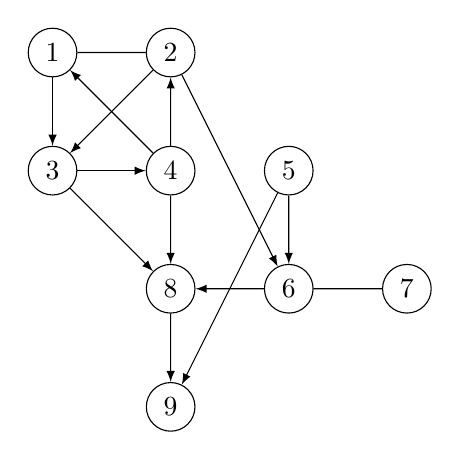
\begin{tikzpicture}[scale=1.5]
	\node[draw, shape=circle] (1) at (0,1) {1};
	\node[draw, shape=circle] (2) at (1,1) {2};
	\node[draw, shape=circle] (3) at (0,0) {3};
	\node[draw, shape=circle] (4) at (1,0) {4};
	
	\draw (1) -- (2);
	\draw[-latex] (1) -- (3);
	\draw[-latex] (4) -- (1);
	\draw[-latex] (2) -- (3);
	\draw[-latex] (4) -- (2);
	\draw[-latex] (3) -- (4);

	\node[draw, shape=circle] (5) at (2,0) {5};
	\node[draw, shape=circle] (6) at (2,-1) {6};
	\node[draw, shape=circle] (7) at (3,-1) {7};
	\node[draw, shape=circle] (8) at (1, -1) {8};
	\node[draw, shape=circle] (9) at (1, -2) {9};

	\draw[-latex] (2) -- (6);
	\draw[-latex] (3) -- (8);
	\draw (6) -- (7);
	\draw[-latex] (5) -- (6);
	\draw[-latex] (5) -- (9);
	\draw[-latex] (4) -- (8);
	\draw[-latex] (6) -- (8);
	\draw[-latex] (8) -- (9);
\end{tikzpicture}
\caption{The graph $D$ in Exercise \ref{exerc:example_D}.} \label{fig:example_D}
\end{figure}




\item Prove that if $D$ is acyclic, then $D$ has a source. Conclude that $D$ can be topologically sorted.

\item Prove that if $D$ is simple, then $\tau(D) \le 2 \mu(D)$.

\item Prove that if $I$ is a minimum feedback vertex set of $D$, then for any $v \in I$, there is a cycle in $D$ whose only vertex in $I$ is $v$.

\item Prove that if $H \subseteq D$, then
\begin{align*}
	\packing(H) &\le \packing(D),\\
	\feedback(H) &\le \feedback(D),\\
	\clique(H) &\le \clique(D).
\end{align*}
For which other numbers reviewed in Section \ref{sec:graphs} do we have a similar inequality?

\item Prove that $\packing(D) \le \feedback(D)$, $\girth(D) \packing(D) \le n$ and that $\girth(D) \le n - \feedback(D) + 1$.



%%%%%%% Simple graphs



\item \label{exerc:example_simple_D} Let $D_1$ and $D_2$ be the simple connected graphs depicted in Figure \ref{fig:example_simple_D}. For $i=1,2$, determine $\matching(D_i)$, $\feedback(D_i)$, $\chromatic(D_i)$, $\clique(D_i)$, $\cliqueCover(D_i)$, and draw $\bar{D_i}$.

\begin{figure}
\centering
	\subfloat[$D_1$]
	{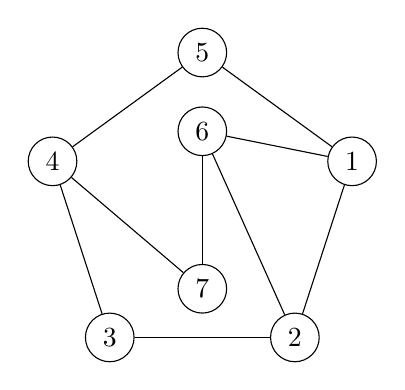
\begin{tikzpicture}
	\tikzstyle{every node}=[draw,shape=circle];

	\node (1) at (90-72*1:2) {1};
	\node (2) at (90-72*2:2) {2};
	\node (3) at (90-72*3:2) {3};
	\node (4) at (90-72*4:2) {4};
	\node (5) at (90-72*5:2) {5};	
	
    \draw (1) -- (2);
    \draw (2) -- (3);
    \draw (3) -- (4);
    \draw (4) -- (5);
    \draw (5) -- (1);

	\node (6) at (0,1) {6};
	\node (7) at (0,-1) {7};
	
	\draw (6) -- (7);
	
	\draw (6) -- (1);
	\draw (6) -- (2);
	\draw (7) -- (4);
	\end{tikzpicture}} \hspace{1cm}
	\subfloat[$D_2$]
	{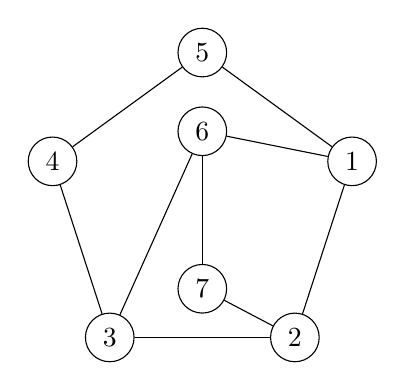
\begin{tikzpicture}
	\tikzstyle{every node}=[draw,shape=circle];

	\node (1) at (90-72*1:2) {1};
	\node (2) at (90-72*2:2) {2};
	\node (3) at (90-72*3:2) {3};
	\node (4) at (90-72*4:2) {4};
	\node (5) at (90-72*5:2) {5};	
	
    \draw (1) -- (2);
    \draw (2) -- (3);
    \draw (3) -- (4);
    \draw (4) -- (5);
    \draw (5) -- (1);

	\node (6) at (0,1) {6};
	\node (7) at (0,-1) {7};
	
	\draw (6) -- (7);
	
	\draw (6) -- (1);
	\draw (6) -- (3);
	\draw (7) -- (2);
	\end{tikzpicture}}
\caption{The graphs of Exercise \ref{exerc:example_simple_D}.} \label{fig:example_simple_D}
\end{figure}




\item Prove that a simple graph $D$ is bipartite if and only if all its cycles have even length.

\item \label{exerc:independence_max_degree} Prove that a simple graph $D$ with maximum degree $\Delta$ has an independent set of size at least $n/(\Delta + 1)$.






%%%%%% Signed graphs



\item Consider the graph $D$ in Exercise \ref{exerc:example_D}, displayed in Figure \ref{fig:example_D}. For each of the following arc labelling functions $\sigma$, determine the positive and negative packing number, transversal number and girth (six parameters in total) of $(D, \sigma)$:
\begin{exercises}
	\item $\sigma(uv) = 1$ if $|u - v| \le 1$, $\sigma(uv) = -1$ otherwise;
	
	\item $\sigma(uv) = 1$ if $u > v$ and $\sigma(uv) = 0$ otherwise;
	
	\item $\sigma(uv) = -1$ everywhere.	
\end{exercises}


\item Prove that a signed graph with a negative walk from a vertex to itself has a negative cycle.

%\item Prove that a strong signed graph $G$ is balanced if and only if there exists a partition $(I,J)$ of $V$ with the following properties: every arc from $I$ to $J$ or from $J$ to $I$ is negative, and every arc from $I$ to $I$ of from $J$ to $J$ is positive.

\item For any signed graph $G=(V,E)$, let $-G=(V,-E)$ such that $-E = \{ (u,v,-s) : (u,v,s) \in E \}$. Prove that if $G$ has no positive cycles, then $-G$ has no positive cycles of even length and no negative cycles of odd length.

\item Prove that if a signed graph contains, as an unsigned subgraph, an odd undirected cycle, then it contains a positive cycle.

\item Prove that for any set of vertices $I$ and any cycle $C$ in $G$, the $I$-switch preserves the sign of $C$. Conclude that the $I$-switch preserves the positive and negative packing number, transversal number and girth.

\item Verify that the two definitions of the frustration index given in Section \ref{sec:signed_graphs} are indeed equivalent.

\item \MGCOMM{Need to get the right reference for this. Prove that if $G$ is a connected unate simple graph, then $G$ is switch-equivalent to a graph with a positive spanning tree.}


%%%%%% Logical connectives


\item Prove the basic properties of negation, conjunction and disjunction listed in Section \ref{sec:logical_connectives}.

\item \label{exerc:dnf} We shall prove that any Boolean function $\phi : \{0,1\}^n \to \{0,1\}$ can be expressed with negation, conjunction and disjunction.
\begin{exercises}
	\item For any $a \in \{0,1\}^n$, let $\psi^a : \{0,1\}^n \to \{0,1\}$ be defined as
	\[
		\psi^a(x) := \one{ x = a }.
	\]
	A \BF{literal}\index{literal} is either a Boolean variable $x_i$ or its negation $\neg x_i$. Show that $\psi^a$ can be expressed as a conjunction of literals.
	
	\item Verify that
	\[
		\phi(x) = \bigvee_{a : \phi(x) = 1} \psi^a(x).
	\]
	Therefore, $\phi$ can be expressed as a disjunction of conjunctions of literals. This is the so-called \BF{disjunctive normal form}\index{disjunctive normal form}.
	
	\item Prove that any Boolean function $\phi$ can be expressed as conjunction of disjunctions of literals (this is the \BF{conjunctive normal form}\index{conjunctive normal form}).
\end{exercises}

\item Let $x_1 \downarrow x_2 := \neg (x_1 \lor x_2)$. Prove that $\downarrow$ is functionally complete, i.e. any Boolean function $\phi : \{0,1\}^n \to \{0,1\}$ can be expressed using $\downarrow$ and the variables $x_1, \dots, x_n$. Hint: thanks to Exercise \ref{exerc:dnf}, we only need to show that conjunction, disjunction and negation can be expressed using $\downarrow$.

\item The concepts of disjunctive normal form and of functionally complete function can be extended to functions $\phi : \(q\)^n \to \(q\)$ for all $q$. Firstly, show that
\[
	\phi(x) = \max_{a \in \(q\)^n} \left\{ \phi(a) \cdot \min_{v \in [n]} \{ \one{ x_v = a_v } \} \right\}.
\]
Secondly, prove that $x_1 \downarrow x_2 := \min\{x_1 ,x_2 \} + 1$ is functionally complete (we perform all operations mod $q$). You can do so by showing that the following functions can be expressed using $\downarrow$ and the appropriate variables:
\begin{exercises}
	\item $x_1 + a$ for any $a \in \(q\)$;
	\item $\min\{ x_1, x_2 \}$;
	\item any constant function $a \in \(q\)$;
	\item $\one{ x_1 = a}$ for any $a \in \(q\)$;
	\item $b \cdot \one{ x_1 = a }$ for any $a,b \in \(q\)$;
	\item any function $\psi(x_1)$ of one variable;
	\item $\max\{x_1, x_2\}$;
	\item finally, any function $\phi(x)$.
\end{exercises}



%%%%%% Groups and semigroups




\item \label{exerc:generating_sets_symmetric_group} Prove that the following are generating sets of $\Sym([m])$:
\begin{exercises}
	\item the set of all cyclic permutations $\pi = (a_1 \espace a_2 \dots \espace a_k)$ for all $2 \le k \le m$, where
	\[
		\pi(a_1) = a_2, \dots, \pi(a_{k-1}) = a_k, \pi(a_k) = a_1,
	\]
	and $\pi$ fixes all other elements of $[m]$;
	
	\item the set of all transpositions of $[m]$;
	
	\item \label{it:coxeter_generators} the \BF{Coxeter generators}\index{Coxeter generators}:
	\[
		\{ (1 \espace 2), (2 \espace 3), \dots, (m-1 \espace m) \};
	\]
	
	\item these two permutations: $\{ (1 \espace 2), (1 \espace 2 \espace \dots \espace m) \}$.
\end{exercises}

\item Let $S$ be a set of transpositions in $\Sym([m])$. Prove that $S$ is a generating set of $\Sym([m])$ if and only if the simple graph $([m], \{ uv : (u \espace v) \in S\} )$ is connected.

\item Prove that the alternating group $\Alt(B)$ is generated by the set of all 3-cycles.

\item \label{exerc:generating_sets_tran} Let $B$ be a finite set. Prove that if $T$ is a generating set of $\Sym(B)$ and $f$ is any transformation of $B$ of rank $|B|-1$, then $T \cup f$ is a generating set of $\Tran(B)$.


\item \label{exerc:rank} Let $B$ be a finite set. Prove that for any $f, g \in \Tran(B)$, 
\[
	\rank(f) + \rank(g) - |B| \le \rank(f \circ g) \le \min\{\rank(f), \rank(g)\}.
\]

\item The kernel of $f \in \Tran(B)$ is the partition of $B$ into pre-images of $B$. The analogue of the upper bound on the rank in Exercise \ref{exerc:rank} for kernels is as follows. Let $P = \{P_1, \dots, P_a\}$ and $Q = \{Q_1, \dots, Q_b\}$  be two partitions of the same set $B$, then $Q$ is a \BF{refinement}\index{refinement} of $P$ (denoted by $P \le Q$) if for every part $Q_j$ of $Q$, there exists a part $P_i$ of $P$ such that $Q_j \subseteq P_i$. Prove that $\ker(f \circ g) \le \ker(g)$. Do we always have $\ker(f \circ g) \le \ker(f)$?


\item This exercise is about generating sets of $\Sing([m])$ of minimum size (see the seminal work by Howie \cite{How66, How78}).
\begin{exercises}
	\item Prove that any generating set of $\Sing([m])$ has at least $\binom{m}{2}$ elements.
	
	\item Prove that the set of all assignments $A := \{ (a \to b) : a,b \in [m], a \ne b \}$ is a generating set of $\Sing([m])$.
	
	\item Any set of assignments $X \subseteq A$ can be represented by a loopless digraph $D_X = ([m], E_X)$, where $ab \in E$ if and only if  $(a \to b) \in E_X$. Prove that if $D_X$ is a strong tournament, then $X$ is a generating set of $\Sing([m])$ (and is of minimum size).
	
	\item Conversely, show that $X \subseteq A$ is a generating set of $\Sing([m])$ of minimum size only if $D_X$ is a strong tournament.
\end{exercises}

\item Say a transformation $f$ of $[m]$ is monotone if $x \le y$ implies $f(x) \le f(y)$.
\begin{exercises}
	\item Verify that monotone transformations form a subsemigroup of $\Tran([m])$.
	
	\item Show that this semigroup is generated by its idempotents.
	
	\item Repeat the previous two items for increasing transformations, for which $x \le f(x)$.
\end{exercises}


%%%%% Finite fields




\item Give the addition and multiplication tables for $\GF(7)$.

\item Give the conversion exponential-polynomial (like what we did for $\GF(4)$ and $\GF(8)$) for $\GF(16)$ generated by $x^4 + x + 1$ and for $\GF(9)$ generated by $x^2 + x + 2$.

\item Let $\GF(q)$ have characteristic $p$ and $\beta, \gamma \in \GF(q)$. Prove that
\[
	(\beta + \gamma)^p = \beta^p + \gamma^p.
\]

\item For any prime power $q$, exhibit $n \ge 2$ and $x \in \GF(q)^n$ such that $x \ne 0$ and $x \cdot x = 0$.

\item Prove that the number of subspaces of $\GF(q)^n$ of dimension $k$ is given by the Gaussian binomial
\[
	\binom{n}{k}_q = \prod_{i=0}^{k-1} \frac{ q^n - q^i }{ q^k - q^i }.
\]

\item \label{exerc:GL} Prove that for any $q$ and $n$,
\[
	|\GL(n,q)| = \prod_{i=0}^{n-1} (q^n -q^i).
\]
More generally, prove that the number of $m \times n$ matrices over $\GF(q)$ with rank $r$ is given by
\[
	\prod_{i=0}^{r-1} \frac{q^m - q^i}{q^r - q^i} (q^n - q^i).
\]






%%%%% Hamming and Manhattan metrics



\item Prove that if $x,y \in \{0,1\}^n$ have the same Hamming weight, then their Hamming distance is even.

\item Prove that the Hamming distance is a metric, i.e. for all $x,y,z \in \(q\)^n$:
\begin{alignat*}{2}
	\dH(x,y) &\ge 0,\\
	\dH(x,y) &= \dH(y,x),\\
	\dH(x,y) &= 0 \text{ if and only if } x=y,\\
	\dH(x,y) &\le \dH(x,z) + \dH(z,y) &\qquad& \text{triangular inequality}.
\end{alignat*}
Repeat for the Manhattan distance.

\item Show that the Hamming graph satisfies $d(H(n,q)) = n (q-1)$, $\clique(H(n,q)) = q$ and $\independence(H(n,q)) = q^{n-1}$.

\item Prove that $\phi$ is an automorphism of the Hamming graph if and only if it is an isometry of the Hamming metric. What about automorphisms of the Grid graph vs isometries of the Manhattan metric?


\item Determine the following properties of the grid graph $\mathrm{Grid}(n,q)$;
\begin{exercises}
	\item its minimum, maximum and average degree;
	
	\item its chromatic number, its clique number and its independence number.
\end{exercises}

\item Give a recursive construction of a cyclic $(n,q)$-Gray code for all $n$ and $q$.

\item Prove that for any $n$ and $q$, there is a Gray code $x^0, \dots, x^{q^n-1}$ such that $\dManhattan(x^i, x^{i+1}) = 1$ for all $0 \le i \le q^n-2$ (see \cite{Gua98}).


%%%%%%%% Error-correcting codes



\item \label{exerc:Gilbert_bound} Prove the Gilbert bound (hint: use Exercise \ref{exerc:independence_max_degree}) and the sphere-packing bound.


\item Determine the respective minimum distances of the repetition code and of the parity-check code directly from their definition.

\item For which values of $q$ and $n$ does the $q$-ary repetition code of length $n$ reach the sphere-packing bound? What about the parity-check code?


\item Verify that if $\mathcal{C}$ is a linear code, then 
\[
	\dmin(\mathcal{C}) = \min\{ \wH(c) : c \in \mathcal{C}, c \ne 0 \}.
\]
Conclude that $\dmin(\mathcal{C})$ is indeed the minimum number of linearly dependent columns of its parity-check matrix ${\bf H}$.

\item Determine all the binary MDS codes.

\item \label{exerc:Hamming_codes} This exercise is about Hamming codes.
\begin{exercises}
	\item Verify that the Hamming code with redundancy $2$ is the binary repetition code of length $3$.

	\item Prove that the minimum distance of the Hamming code with redundancy $r$ is $3$ for all $r \ge 2$.

	\item Verify that Hamming codes reach the sphere-packing bound.

	\item We can extend the construction to any $\GF(q)$. For any prime power $q$ and any integer $r \ge 2$, design the parity-check matrix of the $q$-ary Hamming code with redundancy $r$. This code must have minimum distance three for all values of $q$ and $r$ and has to reach the sphere-packing bound.
\end{exercises}

\item \label{exerc:RS} This exercise is about Reed-Solomon codes.
\begin{exercises}
	\item Prove that the Reed-Solomon code $\mathcal{RS}(n,k)$ has minimum distance $n-k+1$.

	\item Prove that its generator matrix is
	\[
	{\bf G}_{\mathcal{RS}(n,k)} = \begin{pmatrix}
	1 & 1 & \dots & 1\\
	1 & \alpha & \dots & \alpha^{n-1}\\
	\vdots & \vdots & \dots & \vdots\\
	1 & \alpha^{k-1} & \dots & \alpha^{(k-1)(n-1)}
	\end{pmatrix}.
	\]

	\item The extended Reed-Solomon code $\mathcal{ERS}(n+1,k)$ uses evaluations over all elements of $\GF(q)$, i.e. it uses $y^P = (P(0), x^P) \in \GF(q)^{n+1}$ instead of $x^P$. Is $\mathcal{ERS}(n+1,k)$ an MDS code? What is its generator matrix?
\end{exercises}









\end{exercises}


\chapter{Introduction to Finite Dynamical Systems} \label{ch:introduction}




This introductory chapter has several aims. Firstly, we give some simple examples of how we may encounter Finite Dynamical Systems in other areas. Secondly, we introduce the notation, terminology and conventions used throughout the book. Thirdly, we give a glimpse of the sort of problems in which we will be interested in the following chapters.

We shall be going from less formal to more formal. The reader is reminded of the review of essential mathematical background in Chapter \ref{ch:mathematical_background}.




\section{Preliminary examples} \label{sec:preliminary examples}

\subsection{Hat game} \label{sec:hat_game_example}

Let us begin with an example of a cooperative game. Consider a team of two players, competing against an adversary. The adversary chooses a hat for each player, which can be blue or red. Each player cannot see their own hat, but can see the other player's. Both players have to make a guess about their own hat's colour; these guesses are simultaneous and the players are not allowed to communicate once they wear their hats. However, they are allowed to agree upon a common guessing strategy beforehand. The team wins if, whatever the adversary chose, at least one of the players guessed the right colour for their own hat.

An example of losing strategy is when both players guess ``I guess the colour that I see,'' or in other words ``I guess that we have the same colour.'' If both players use that strategy, then here is what happens (correct guessses are in bold):
~\\
\begin{center}
\begin{tabular}{|c|c||c|c|}
	\hline
	\multicolumn{2}{|c||}{Hat colours} & \multicolumn{2}{|c|}{Guesses}\\
	\hline
	Player 1 & Player 2 & Player 1 & Player 2\\
	\hline
	Blue 	& Blue & \textbf{Blue} 	& \textbf{Blue} 	\\
	Blue 	& Red  & Red 			& Blue 	\\
	Red 	& Blue & Blue 			& Red 	\\
	Red 	& Red  & \textbf{Red} 	& \textbf{Red} 	\\
	\hline
\end{tabular}
\end{center}
~\\
When the hats have different colours, then both players guess incorrectly, and hence the team loses.

An example of a winning strategy is that the first player guesses that both players have the same colour, while the second player guesses they have different colours. Clearly, exactly one of them is right each time, as seen below:
~\\
\begin{center}
\begin{tabular}{|c|c||c|c|}
	\hline
	\multicolumn{2}{|c||}{Hat colours} & \multicolumn{2}{|c|}{Guesses}\\
	\hline
	Player 1 & Player 2 & Player 1 & Player 2\\
	\hline
	Blue 	& Blue & \textbf{Blue} 	& Red 	\\
	Blue 	& Red  & Red 			& \textbf{Red} 	\\
	Red 	& Blue & Blue 			& \textbf{Blue} 	\\
	Red 	& Red  & \textbf{Red} 	& Blue 	\\
	\hline
\end{tabular}
\end{center}
~\\
Let us re-write this winning example in the formalism that we shall use throughout this book. Instead of B and R, let the colours be taken from the set $\{0,1\}$; denote the players as $1$ and $2$, the colour of their hats as $x_1$ and $x_2$, and their guessing strategies as $f_1(x_2)$ and $f_2(x_1)$ (the guessing strategy of player $1$ only depends on the colour of the hat of player $2$ and vice versa). Our problem was then to find $f(x) = (f_1(x_2), f_2(x_1)) : \{0,1\}^2 \to \{0,1\}^2$ such that for all $x = (x_1, x_2) \in \{0,1\}^2$, either $f_1(x_2) = x_1$ or $f_2(x_1) = x_2$. the correct solution was then given by
\[
	f_1(x_2) = x_2, \quad f_2(x_1) = x_1 + 1 \mod 2.
\]
More concretely, we have
\begin{center}
\begin{tabular}{|c|c|}
	\hline
	$x$ & $f(x)$\\
	\hline
	00 & 01\\
	01 & 11\\
	10 & 00\\
	11 & 10\\
	\hline
\end{tabular}
\end{center}


We can then generalise the hat game to $n$ players and $n$ hat colours as follows: we are searching for
\[
	f(x) = (f_1(x_2, \dots, x_n), f_2(x_1, x_3, \dots, x_n), \dots, f_n(x_1, \dots, x_{n-1})) : \{0,1, \dots, n-1\}^n \to \{0,1,\dots,n-1\}^n
\]
such that for any $x \in \{0,1, \dots, n-1\}^n$, there exists $1 \le v \le n$ such that $f_v(x_1, \dots, x_{v-1}, x_{v+1}, \dots, x_n) = x_v$. This time the guess can be ``Player $v$ guesses that the sum of all hat colours is equal to $v$ (modulo $n$),'' or in other words:
\[
	f_v(x) = v - \sum_{u \ne v} x_u \mod n.
\]
Again, for any $x$ exactly one player will guess correctly (namely, the player $v$ such that $v = \sum_{u = 1}^n x_u \mod n$), and the team wins.




\subsection{Rumour spreading} \label{sec:rumour}

Let us consider a toy example of rumour spreading. Say there are seven acquaintances (whom we shall simply refer to as person $1$ to $7$), not all of them being friends. A rumour spreads in the wider population and reaches one of those acquaintances. Using the Boolean variable $x_v$ to denote whether person $v$ believes in that rumour, the influences of different people are given as below.

\begin{align*}
	f_1(x) &= x_1 \land (x_2 \lor \neg x_3)\\
	f_2(x) &= x_2 \lor (x_1 \land x_3)\\
	f_3(x) &= \mathrm{majority}( x_1, x_2, x_4 )\\
	f_4(x) &= x_4 \lor x_3 \lor (x_5 \land \neg x_6)\\
	f_5(x) &= \mathrm{majority}( x_4, x_6, \neg x_7 )\\
	f_6(x) &= \left( x_6 \land ( x_4 \lor x_7 ) \right) \lor ( x_4 \land x_5 )\\
	f_7(x) &= \neg x_5 \lor x_6.
\end{align*}

The majority function returns $1$ if two or more variables are equal to $1$, and $0$ otherwise. The logical connectives $\land$, $\lor$ and $\neg$ (conjunction, disjunction and negation respectively) are reviewed in Section \ref{sec:logical_connectives}. Of course, those behaviours are simplistic (person $3$ acts in a sheepish manner, for instance), but they reflect trust in friends (if $1$ and $3$ both believe in the rumour, then so will $2$), or distrust (if $5$ does not believe in the rumour, then $7$ will).

A schematic view of this network of people is given in Figure \ref{fig:rumour_IG} below.

\begin{figure}
\centering
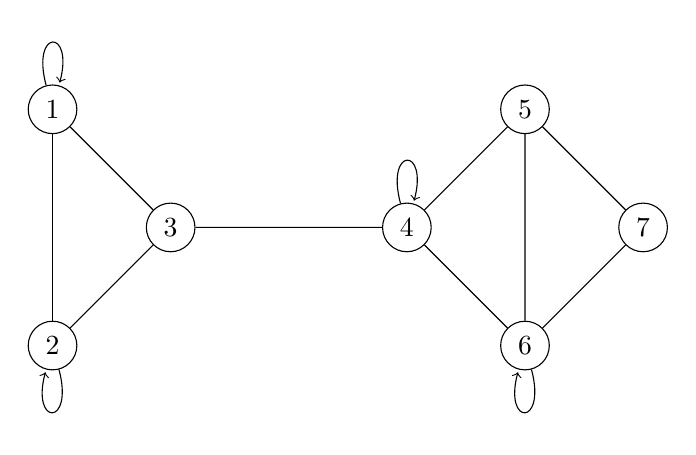
\begin{tikzpicture}[scale=1.5]
	\tikzstyle{every node}=[draw, shape=circle];

	\node (1) at (0,2) {1};
	\node (2) at (0,0) {2};
	\node (3) at (1,1) {3};
	\node (4) at (3,1) {4};
	\node (5) at (4,2) {5};
	\node (6) at (4,0) {6};
	\node (7) at (5,1) {7};
	
	\path (1) edge (2)
	(1) edge (3)
	(2) edge (3)
	(3) edge (4)
	(4) edge (5)
	(4) edge (6)
	(5) edge (6)
	(5) edge (7)
	(6) edge (7)
	(1) edge [loop above] (1)
	(2) edge [loop below] (2)
	(4) edge [loop above] (4)
	(6) edge [loop below] (6);	
\end{tikzpicture}
\caption{The network of acquaintances from Section \ref{sec:rumour}.} \label{fig:rumour_IG}
\end{figure}


Can one single person spread the rumour across the set of acquaintances? If all opinions are updated at the same time, then the answer is ``no.'' Indeed, Figure \ref{fig:rumour_trajectories} illustrates the evolution of the opinions when they start at a state where either no one believes (the state $0000000$) or a single person believes in the rumour (the states $1000000$ to $0000001$). None of these trajectories leads to the state $1111111$ where everyone believes in the rumour.

More can be said about this example, and in fact Exercise \ref{exerc:rumour} asks you to prove the following claims:
\begin{enumerate}
	\item There exists a set of only two people $\{u,v\}$ such that if $u$ and $v$ are the only two people believing in the rumour at some point, then eventually everyone will believe.
	
	\item Even if opinions are not updated at the same time, there is no way that a single believer can spread the rumour to all the acquaintances.
\end{enumerate}


\begin{figure}
\centering
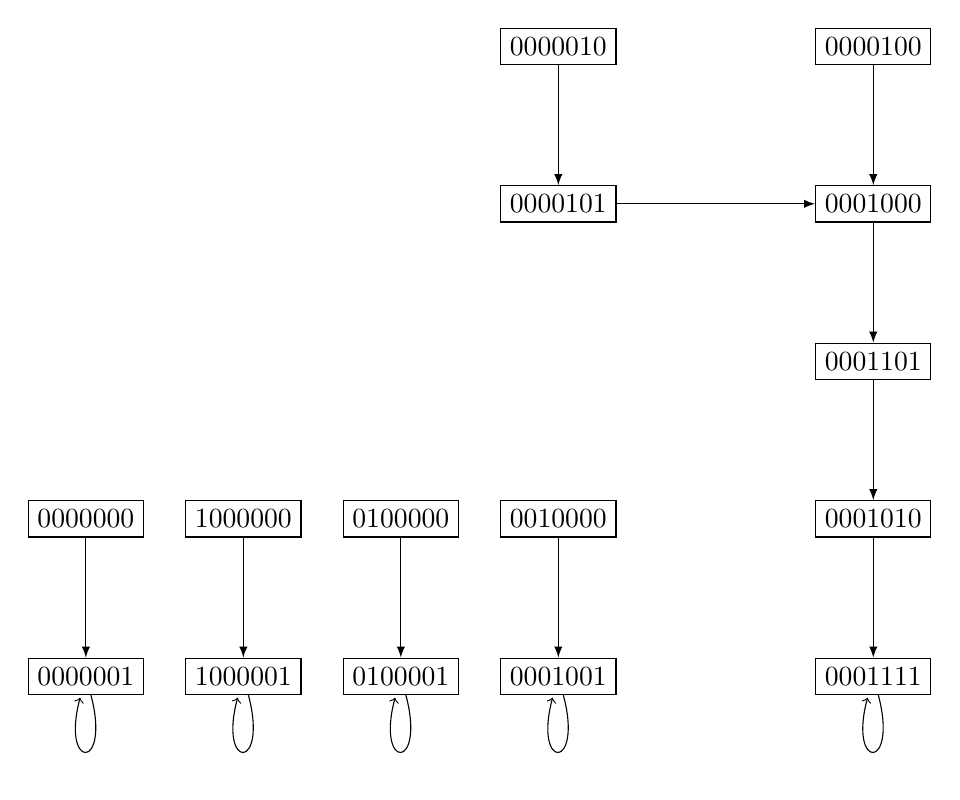
\begin{tikzpicture}[scale=2]
	\tikzstyle{every node}=[draw];

	\node (0) 		at (0,1) {0000000};
	\node (1) 		at (1,1) {1000000};
	\node (2) 		at (2,1) {0100000};
	\node (3) 		at (3,1) {0010000};
	\node (4) 		at (5,3) {0001000};
	\node (5) 		at (5,4) {0000100};
	\node (6) 		at (3,4) {0000010};
	\node (7) 		at (0,0) {0000001};
	
	\node (17) 		at (1,0) {1000001};
	\node (27) 		at (2,0) {0100001};
	\node (47) 		at (3,0) {0001001};
	\node (57) 		at (3,3) {0000101};
	
	\node (457) 	at (5,2) {0001101};
	\node (46) 		at (5,1) {0001010};
	\node (4567) 	at (5,0) {0001111};
	
	
	
	\path (0) edge[-latex] (7)
	(1) edge[-latex] (17)
	(2) edge[-latex] (27)
	(3) edge[-latex] (47)
	(4) edge[-latex] (457)
	(457) edge[-latex] (46)
	(46) edge[-latex] (4567)
	(5) edge[-latex] (4)
	(6) edge[-latex] (57)
	(57) edge [-latex] (4)
	(7) edge [loop below] (7)
	(17) edge [loop below] (17)	
	(27) edge [loop below] (27)
	(47) edge [loop below] (47)
	(4567) edge [loop below] (4567)
	;
	
\end{tikzpicture}
\caption{Trajectories of beliefs in the rumour.} \label{fig:rumour_trajectories}
\end{figure}



\section{Motivation and examples} \label{sec:motivation_and_examples}

The main topic of this book is the study of functions of the form $f: \{0,\dots,q-1\}^n \to \{0,\dots,q-1\}^n$. In order to illustrate what we may want to know about them, we shall use the following example.


\begin{example}\label{ex:monotone_vecC5}
Let $f : \{0,1\}^5 \to \{0,1\}^5$, $f = (f_1, \dots, f_5)$ where
\begin{align*}
	f_1(x) &= x_1 \land x_5\\
	f_2(x) &= x_2 \lor x_1\\
	f_3(x) &= x_3 \land x_2\\
	f_4(x) &= x_4 \land x_3\\
	f_5(x) &= x_5 \lor x_4.
\end{align*}
	
The dynamics are given in Figure \ref{fig:monotone_vecC5}. As we can see, all the states end up at a fixed point.

\begin{figure}
\centering
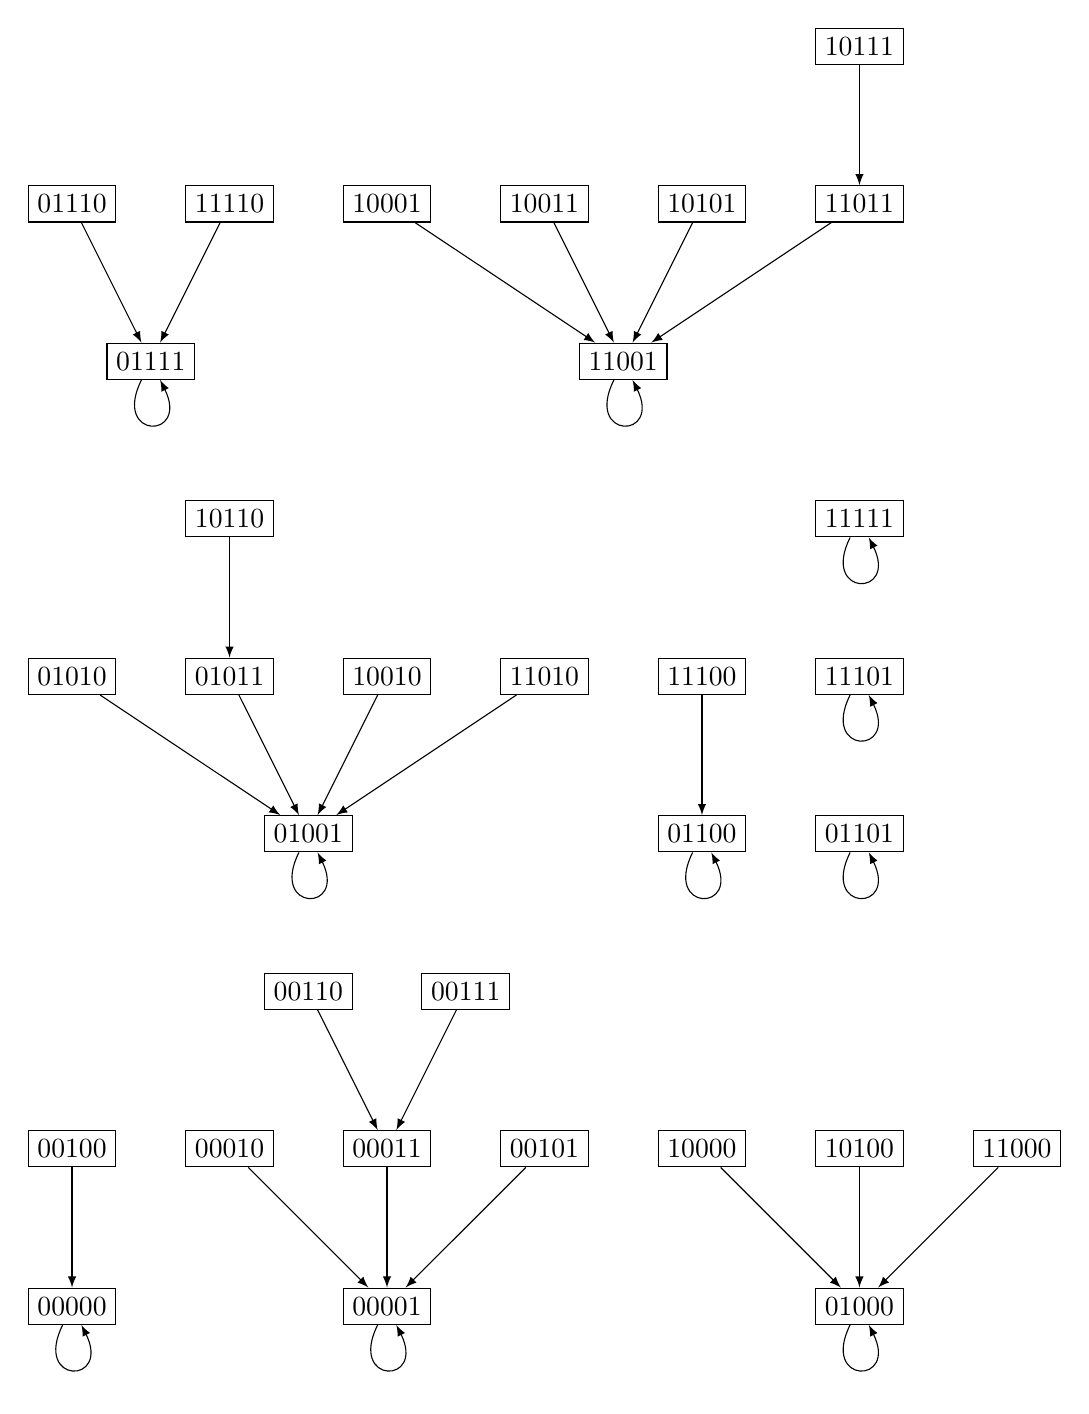
\begin{tikzpicture}
	\tikzstyle{every node}=[draw];

	\node (0) at (0,0) {00000};
	\node (1) at (4,0) {00001};
	\node (2) at (2,2) {00010};
	\node (3) at (4,2) {00011};
	\node (4) at (0,2) {00100};
	\node (5) at (6,2) {00101};
	\node (6) at (3,4) {00110};
	\node (7) at (5,4) {00111};
	
	\node (8) at (10,0) {01000};
	\node (9) at (3,6) {01001};
	\node (10) at (0,8) {01010};
	\node (11) at (2,8) {01011};
	\node (12) at (8,6) {01100};
	\node (13) at (10,6) {01101};
	\node (14) at (0,14) {01110};
	\node (15) at (1,12) {01111};
	
	\node (16) at (8,2) {10000};
	\node (17) at (4,14) {10001};
	\node (18) at (4,8) {10010};
	\node (19) at (6,14) {10011};
	\node (20) at (10,2) {10100};
	\node (21) at (8,14) {10101};
	\node (22) at (2,10) {10110};
	\node (23) at (10,16) {10111};
	
	\node (24) at (12,2) {11000};
	\node (25) at (7,12) {11001};
	\node (26) at (6,8) {11010};
	\node (27) at (10,14) {11011};
	\node (28) at (8,8) {11100};
	\node (29) at (10,8) {11101};
	\node (30) at (2,14) {11110};
	\node (31) at (10,10) {11111};

	\draw[-latex] (0) .. controls(-0.5, -1) and (0.5, -1) .. (0);
	\draw[-latex] (4) -- (0);

	\draw[-latex] (1) .. controls(3.5, -1) and (4.5, -1) .. (1);
	\draw[-latex] (2) -- (1);
	\draw[-latex] (3) -- (1);
	\draw[-latex] (5) -- (1);
	\draw[-latex] (6) -- (3);
	\draw[-latex] (7) -- (3);

	\draw[-latex] (8) .. controls(9.5, -1) and (10.5, -1) .. (8);
	\draw[-latex] (24) -- (8);
	\draw[-latex] (16) -- (8);
	\draw[-latex] (20) -- (8);

	\draw[-latex] (9) .. controls(2.5, 5) and (3.5, 5) .. (9);
	\draw[-latex] (10) -- (9);
	\draw[-latex] (11) -- (9);
	\draw[-latex] (18) -- (9);
	\draw[-latex] (26) -- (9);
	\draw[-latex] (22) -- (11);

	\draw[-latex] (12) .. controls(7.5, 5) and (8.5, 5) .. (12);
	\draw[-latex] (28) -- (12);

	\draw[-latex] (13) .. controls(9.5, 5) and (10.5, 5) .. (13);

	\draw[-latex] (15) .. controls(0.5, 11) and (1.5, 11) .. (15);
	\draw[-latex] (14) -- (15);
	\draw[-latex] (30) -- (15);

	\draw[-latex] (25) .. controls(6.5, 11) and (7.5, 11) .. (25);
	\draw[-latex] (17) -- (25);
	\draw[-latex] (19) -- (25);
	\draw[-latex] (21) -- (25);
	\draw[-latex] (27) -- (25);
	\draw[-latex] (23) -- (27);

	\draw[-latex] (29) .. controls(9.5, 7) and (10.5, 7) .. (29);

	\draw[-latex] (31) .. controls(9.5, 9) and (10.5, 9) .. (31);
\end{tikzpicture}
\caption{The dynamics of $f$ from Example \ref{ex:monotone_vecC5}}\label{fig:monotone_vecC5}
\end{figure}	
\end{example}	


\begin{figure}[!htp]
\centering
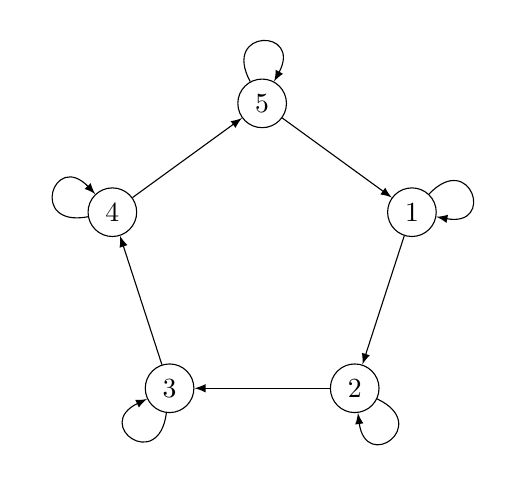
\begin{tikzpicture}
	\tikzstyle{every node}=[draw, shape=circle];

	\foreach \x in {1,...,5}{
		\node (\x) at (90-72*\x:2) {$\x$};
		\draw[-latex] (\x) .. controls(90-72*\x+10:3) and (90-72*\x-10:3) .. (\x);
	}

	\draw[-latex] (1) -- (2);
	\draw[-latex] (2) -- (3);
	\draw[-latex] (3) -- (4);
	\draw[-latex] (4) -- (5);
	\draw[-latex] (5) -- (1);
\end{tikzpicture}
\caption{Interaction graph $\IG(f)$.}
\label{fig:IG_vecC5}
\end{figure}


Obviously, since $\{0,\dots,q-1\}^n$ is a finite set, given a full description of $f$ and enough time, we can understand everything about it. However, in many cases either we do not know everything about $f$ or we can select some properties of $f$. The main aim of this book is to determine the dynamical properties of $f$ when only given some of its structural properties. We can highlight four main structural properties, informally given as follows.

\begin{enumerate}
	\item The interaction graph $\IG(f)$.\\
	This graph (already seen in Figure \ref{fig:rumour_IG}) indicates the underlying network of interactions. This is arguably the most important parameter, for it is usually well known (while the other parameters) and because it represents the qualitative architecture of the network. As such, Chapters \ref{ch:fixed_points_unsigned} to \ref{ch:stability} are devoted to its influence on different dynamical properties, such as the number of fixed points and of images or the metric stability of the system.
	
	\item The nature of the local functions $f_v$.\\
	Depending  on the situation, we may know that all local functions $f_v$ are linear, monotone, conjunctions of literals, etc. Moreover, focusing on a specific class of local functions may either yield much finer results or help us design FDSs with specific properties. For instance, linear functions will be thoroughly used in Chapter \ref{ch:optimality_feedback}, while Chapter \ref{ch:guessing_number_signed} will make use of conjunctive functions.
	
	\item The alphabet size $q$.\\
	The alphabet size will make a huge difference in some situations, notably the study of (in)stability of FDSs with a given interaction graph in Chapter \ref{ch:stability}. The Boolean case ($q=2$) is the most commonly used, and as such many results will be given for $q=2$ only. However, the Boolean case may be degenerate, as we shall see in a few occasions throughout this book, e.g. in Chapter \ref{ch:periodic_states}.
	
	\item The update schedule $\sigma$.\\
	This is technically not about $f$ per se, but about how it is used by the network. The previous example used the parallel schedule, where $x$ becomes $f(x)$. However, some networks are not synchronised. In those networks, the local updates may occur sequentially, i.e. at each time step only one $x_v$ becomes $f_v(x)$. The influence of the schedule is investigated in Chapters \ref{ch:asynchronous_graph} and \ref{ch:simulation}.
\end{enumerate}


Let us illustrate the influence of those four parameters by modifying the function $f$ from Example \ref{ex:monotone_vecC5} in four different ways. Firstly, let us slightly change the interaction graph.




\begin{example} \label{ex:monotone_C5}
Let us illustrate the influence of interaction graph by keeping the same local functions, but using different variables. We have qualitatively different dynamics, since now a $2$-cycle appears (namely, $01001, 10000$) as seen from Figure \ref{fig:monotone_C5}. 
\begin{align*}
	g_1(x) &= x_2 \land x_5\\
	g_2(x) &= x_3 \lor x_1\\
	g_3(x) &= x_4 \land x_2\\
	g_4(x) &= x_5 \land x_3\\
	g_5(x) &= x_1 \lor x_4
\end{align*}

\begin{figure}[!htp]
\centering
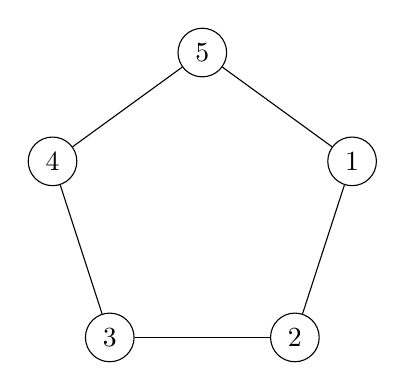
\begin{tikzpicture}
	\tikzstyle{every node}=[draw, shape=circle];

	\foreach \x in {1,...,5}{
		\node (\x) at (90-72*\x:2) {$\x$};
	}

	\draw (1) -- (2);
	\draw (2) -- (3);
	\draw (3) -- (4);
	\draw (4) -- (5);
	\draw (5) -- (1);
\end{tikzpicture}
\caption{Interaction graph $\IG(g)$.}
\label{fig:IG_C5}
\end{figure}

	
\begin{figure}
\centering
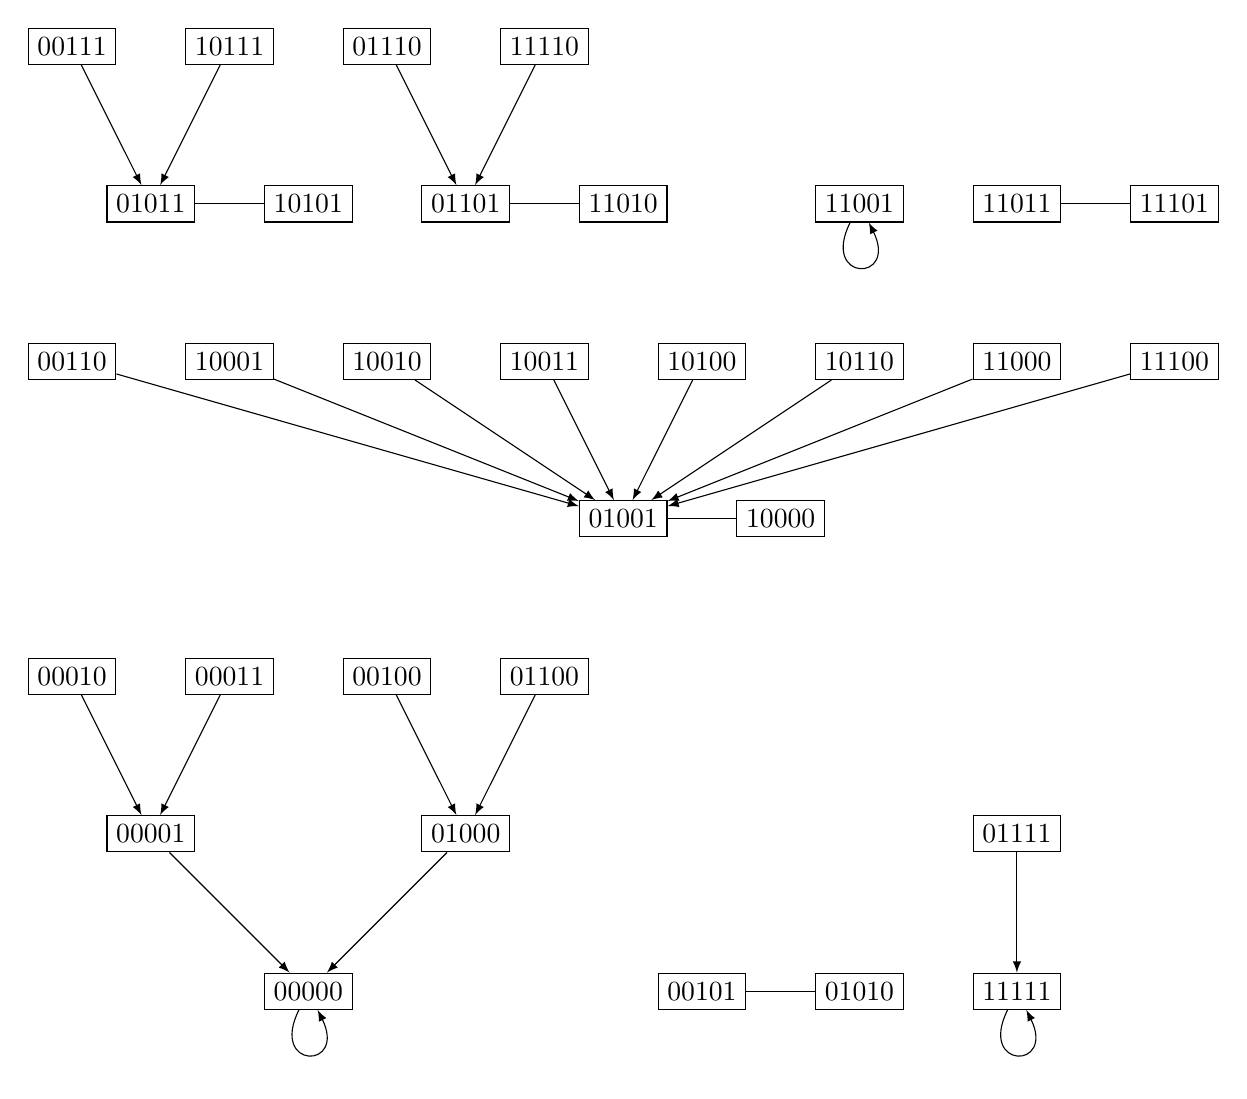
\begin{tikzpicture}
	\tikzstyle{every node}=[draw];

	\node (0) at (3,0) {00000};
	\node (1) at (1,2) {00001};
	\node (2) at (0,4) {00010};
	\node (3) at (2,4) {00011};
	\node (4) at (4,4) {00100};
	\node (5) at (8,0) {00101};
	\node (6) at (0,8) {00110};
	\node (7) at (0,12) {00111};
	
	\node (8) at (5,2) {01000};
	\node (9) at (7,6) {01001};
	\node (10) at (10,0) {01010};
	\node (11) at (1,10) {01011};
	\node (12) at (6,4) {01100};
	\node (13) at (5,10) {01101};
	\node (14) at (4,12) {01110};
	\node (15) at (12,2) {01111};
	
	\node (16) at (9,6) {10000};
	\node (17) at (2,8) {10001};
	\node (18) at (4,8) {10010};
	\node (19) at (6,8) {10011};
	\node (20) at (8,8) {10100};
	\node (21) at (3,10) {10101};
	\node (22) at (10,8) {10110};
	\node (23) at (2,12) {10111};
	
	\node (24) at (12,8) {11000};
	\node (25) at (10,10) {11001};
	\node (26) at (7,10) {11010};
	\node (27) at (12,10) {11011};
	\node (28) at (14,8) {11100};
	\node (29) at (14,10) {11101};
	\node (30) at (6,12) {11110};
	\node (31) at (12,0) {11111};

	\draw[-latex] (0) .. controls(2.5, -1) and (3.5, -1) .. (0);
	\draw[-latex] (1) -- (0);
	\draw[-latex] (8) -- (0);
	\draw[-latex] (2) -- (1);
	\draw[-latex] (3) -- (1);
	\draw[-latex] (4) -- (8);
	\draw[-latex] (12) -- (8);
	
	\draw (5) -- (10);
	
	\draw (9) -- (16);
	\draw[-latex] (6) -- (9);
	\draw[-latex] (17) -- (9);
	\draw[-latex] (18) -- (9);
	\draw[-latex] (19) -- (9);
	\draw[-latex] (20) -- (9);
	\draw[-latex] (22) -- (9);
	\draw[-latex] (24) -- (9);
	\draw[-latex] (28) -- (9);

	\draw (11) -- (21);
	\draw[-latex] (23) -- (11);
	\draw[-latex] (7) -- (11);

	\draw (13) -- (26);
	\draw[-latex] (14) -- (13);
	\draw[-latex] (30) -- (13);

	\draw[-latex] (31) .. controls(11.5, -1) and (12.5, -1) .. (31);
	\draw[-latex] (15) -- (31);

	\draw[-latex] (25) .. controls(9.5, 9) and (10.5, 9) .. (25);

	\draw (27) -- (29);
\end{tikzpicture}
\caption{The dynamics of $g$ from Example \ref{ex:monotone_C5}} \label{fig:monotone_C5}
\end{figure}	
\end{example}


Secondly, every local function $f_v$ of $f$ is of a very particular form: it is either a conjunction or a disjunction of its variables; in particular, it is monotone. A completely different (and yet extremely important) kind of functions is given by linear functions, where the influences are far from monotonic. Linear functions typically yield very structured dynamics. However, as seen below, depending on where it starts, the system can have vastly different dynamics (take $00000$ against $00001$ for instance).




\begin{example} \label{ex:linear_vecC5}
We now illustrate the influence of the nature of the local functions, by considering $h$ below. This FDS is obtained by keeping the same interaction graph as $f$, but then replacing all local functions by their linear counterparts.
\begin{align*}
	h_1(x) &=  x_1 + x_5,\\
	h_2(x) &=  x_1 + x_2,\\
	h_3(x) &=  x_2 + x_3,\\
	h_4(x) &=  x_3 + x_4,\\
	h_5(x) &=  x_4 + x_5,
\end{align*}
where all operations are done modulo $2$. The dynamics are illustrated in Figure \ref{fig:linear_vecC5}: we now have a very long cycle!
\end{example}



\begin{figure}
\centering
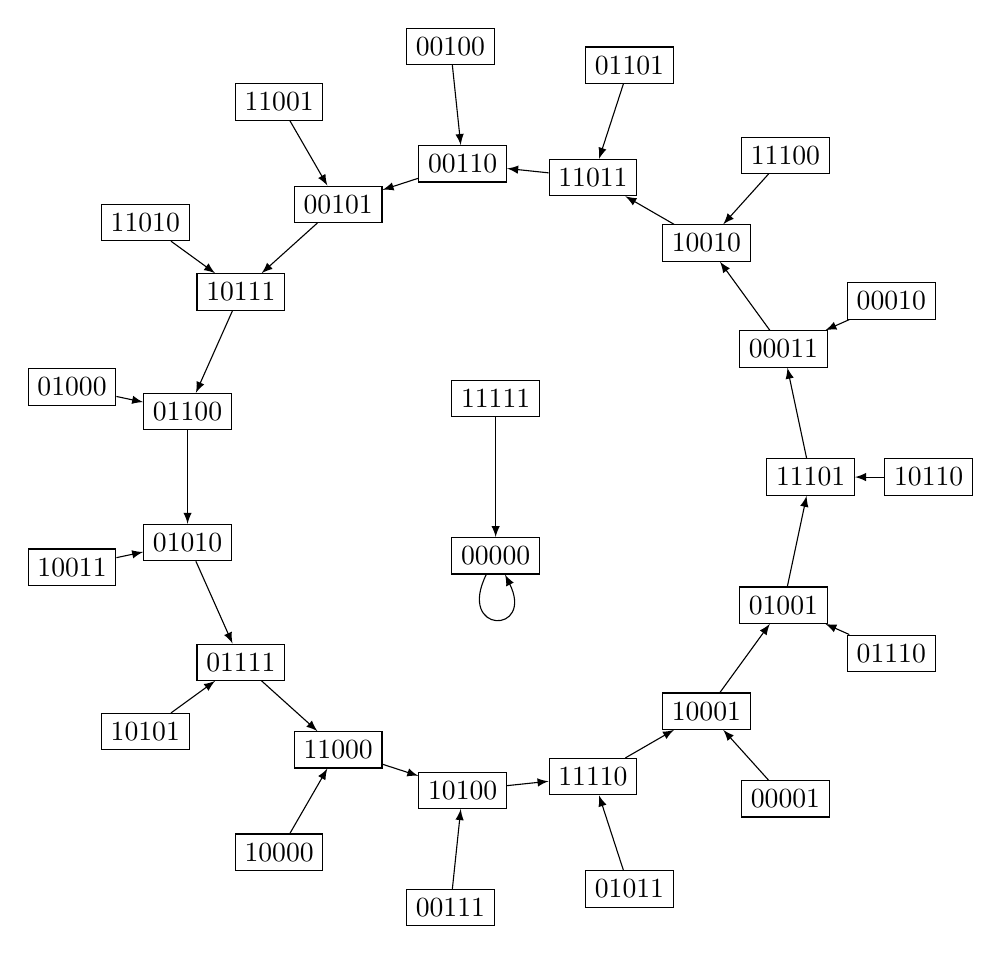
\begin{tikzpicture}
	\tikzstyle{every node}=[draw];

	\node (3) at (1*24:4) {00011};
	\node (18) at (2*24:4) {10010};
	\node (27) at (3*24:4) {11011};
	\node (6) at (4*24:4) {00110};
	\node (5) at (5*24:4) {00101};
	\node (23) at (6*24:4) {10111};
	\node (12) at (7*24:4) {01100};
	\node (10) at (8*24:4) {01010};
	\node (15) at (9*24:4) {01111};
	\node (24) at (10*24:4) {11000};
	\node (20) at (11*24:4) {10100};
	\node (30) at (12*24:4) {11110};
	\node (17) at (13*24:4) {10001};
	\node (9) at (14*24:4) {01001};
	\node (29) at (15*24:4) {11101};
	
	\node (2) at (1*24:5.5) {00010};
	\node (28) at (2*24:5.5) {11100};
	\node (13) at (3*24:5.5) {01101};
	\node (4) at (4*24:5.5) {00100};
	\node (25) at (5*24:5.5) {11001};
	\node (26) at (6*24:5.5) {11010};
	\node (8) at (7*24:5.5) {01000};
	\node (19) at (8*24:5.5) {10011};
	\node (21) at (9*24:5.5) {10101};
	\node (16) at (10*24:5.5) {10000};
	\node (7) at (11*24:5.5) {00111};
	\node (11) at (12*24:5.5) {01011};
	\node (1) at (13*24:5.5) {00001};
	\node (14) at (14*24:5.5) {01110};
	\node (22) at (15*24:5.5) {10110};
	
	\draw[-latex] (2) -- (3);
	\draw[-latex] (28) -- (18);
	\draw[-latex] (13) -- (27);
	\draw[-latex] (4) -- (6);
	\draw[-latex] (25) -- (5);
	\draw[-latex] (26) -- (23);
	\draw[-latex] (8) -- (12);
	\draw[-latex] (19) -- (10);
	\draw[-latex] (21) -- (15);
	\draw[-latex] (16) -- (24);
	\draw[-latex] (7) -- (20);
	\draw[-latex] (11) -- (30);
	\draw[-latex] (1) -- (17);
	\draw[-latex] (14) -- (9);
	\draw[-latex] (22) -- (29);

	\draw[-latex] (3) -- (18);
	\draw[-latex] (18) -- (27);
	\draw[-latex] (27) -- (6);
	\draw[-latex] (6) -- (5);
	\draw[-latex] (5) -- (23);
	\draw[-latex] (23) -- (12);
	\draw[-latex] (12) -- (10);
	\draw[-latex] (10) -- (15);
	\draw[-latex] (15) -- (24);
	\draw[-latex] (24) -- (20);
	\draw[-latex] (20) -- (30);
	\draw[-latex] (30) -- (17);
	\draw[-latex] (17) -- (9);
	\draw[-latex] (9) -- (29);
	\draw[-latex] (29) -- (3);

	\node (0) at (0,-1) {00000};
	\node (31) at (0,1) {11111};
	
	\draw[-latex] (31) -- (0);
	\draw[-latex] (0) .. controls(-0.5, -2) and (0.5, -2) .. (0);
\end{tikzpicture}
\caption{The dynamics of $h$ from Example \ref{ex:linear_vecC5}.}
\label{fig:linear_vecC5}
\end{figure}


Thirdly, changing the alphabet size $q$ could be done in many different ways. A natural example is given below.



\begin{example} \label{ex:3_vecC5}
Let us simply consider the alphabet $\{0, 1, 2\}$ and replace conjunction with minimum and disjunction with maximum:
\begin{align*}
	k_1(x) &= \min\{x_1, x_5\}\\
	k_2(x) &= \max\{x_2, x_1\}\\
	k_3(x) &= \min\{x_3, x_2\}\\
	k_4(x) &= \min\{x_4, x_3\}\\
	k_5(x) &= \max\{x_5, x_4\}.
\end{align*}
It is clear that $k : \{0, 1, 2\}^5 \to \{0, 1, 2\}^5$ reduces to $f$ on $\{0,1\}^5$ (i.e. if all the coordinates of $x$ are either zero or one); this naturally extends to $\{0,2\}^5$ and $\{1,2\}^5$. The courageous reader will attempt to illustrate the dynamics of $k$. 

We can investigate what happens when the alphabet is any $\{0, 1, \dots, q-1\}$ for some $q \ge 2$. An important dynamical property which we can easily determine is that $k$ has period one, or in other words, all states will be eventually mapped to a fixed point. For let $x^1, \dots, x^i \in \{0, \dots, q-1\}^5$ form a cycle of length $i > 1$, i.e. they are all distinct and
\[
	x^2 = k(x^1), \ x^3 = k(x^2), \ \dots, \ x^i = k(x^{i-1}), \ x^1 = k(x^i).
\]
Since $k_1(x) \le x_1$, we have $x^1_1 \le x^i_1 \le \dots \le x^1_1$, hence $x^i_1 = x^1_1$. A similar reasoning holds for all the entities, thus $x^i = x^1$ which is the desired contradiction. We note that the argument above holds for all $q \ge 2$ (and in particular, for $f$). 

However, some properties vary widely with the alphabet size $q$. For instance, the number of fixed points grows as $\Theta(q^5)$ (see Exercise \ref{exerc:number_fixed_points_example}). In general, determining which properties are preserved when the alphabet changes, or how they scale when the alphabet tends to infinity, is a crucial problem throughout this book.
\end{example}

Fourthly, suppose that the entities are not working in parallel any more. Instead, they take turns updating their state. We obtain the following schedule and function.




\begin{example} \label{ex:schedule_vecC5}
In order to show the influence of the schedule, let us use the schedule $\sigma = (1,2,3,4,5)$, where all entities update their states one at a time and in sequence. We then have
\begin{align*}
	f_1^\sigma(x) &= x_1 \land x_5\\
	f_2^\sigma(x) &= x_2 \lor ( x_1 \land x_5 )\\
	f_3^\sigma(x) &= x_3 \land ( x_2 \lor ( x_1 \land x_5 ) )\\
	f_4^\sigma(x) &= x_4 \land ( x_3 \land ( x_2 \lor ( x_1 \land x_5 ) ) )\\
	f_5^\sigma(x) &= x_5 \lor ( x_4 \land ( x_3 \land ( x_2 \lor ( x_1 \land x_5 ) ) ) ) \\
								&= x_5 \lor ( x_4 \land x_3 \land x_2 ).
\end{align*}

We remark that even though $x_1$ first appeared in the definition of $f_5^\sigma$, it actually has no influence on $f_5^\sigma$. As such, there is no arc from $1$ to $5$ in the interaction graph of $f^\sigma$.

In terms of the dynamics, we note that $f$ and $f^\sigma$ have the same set of fixed points (see Figure \ref{fig:schedule_vecC5}); this is a special case of Theorem \ref{th:fixed_points_schedule}.

\begin{figure}[!htp]
\centering
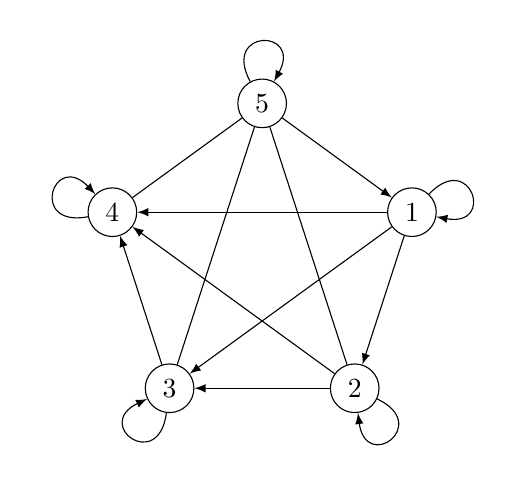
\begin{tikzpicture}
	\tikzstyle{every node}=[draw, shape=circle];

	\foreach \x in {1,...,5}{
		\node (\x) at (90-72*\x:2) {$\x$};
		\draw[-latex] (\x) .. controls(90-72*\x+10:3) and (90-72*\x-10:3) .. (\x);
	}

	\draw[-latex] (1) -- (2);
	\draw[-latex] (1) -- (3);
	\draw[-latex] (1) -- (4);
	\draw[-latex] (2) -- (3);
	\draw[-latex] (2) -- (4);
	\draw (2) -- (5);
	\draw[-latex] (3) -- (4);
	\draw (3) -- (5);
	\draw (4) -- (5);
	\draw[-latex] (5) -- (1);
\end{tikzpicture}
\caption{Interaction graph $\IG(f^\sigma)$.}
\label{fig:IG_fsigma}
\end{figure}

	
\begin{figure}
\centering
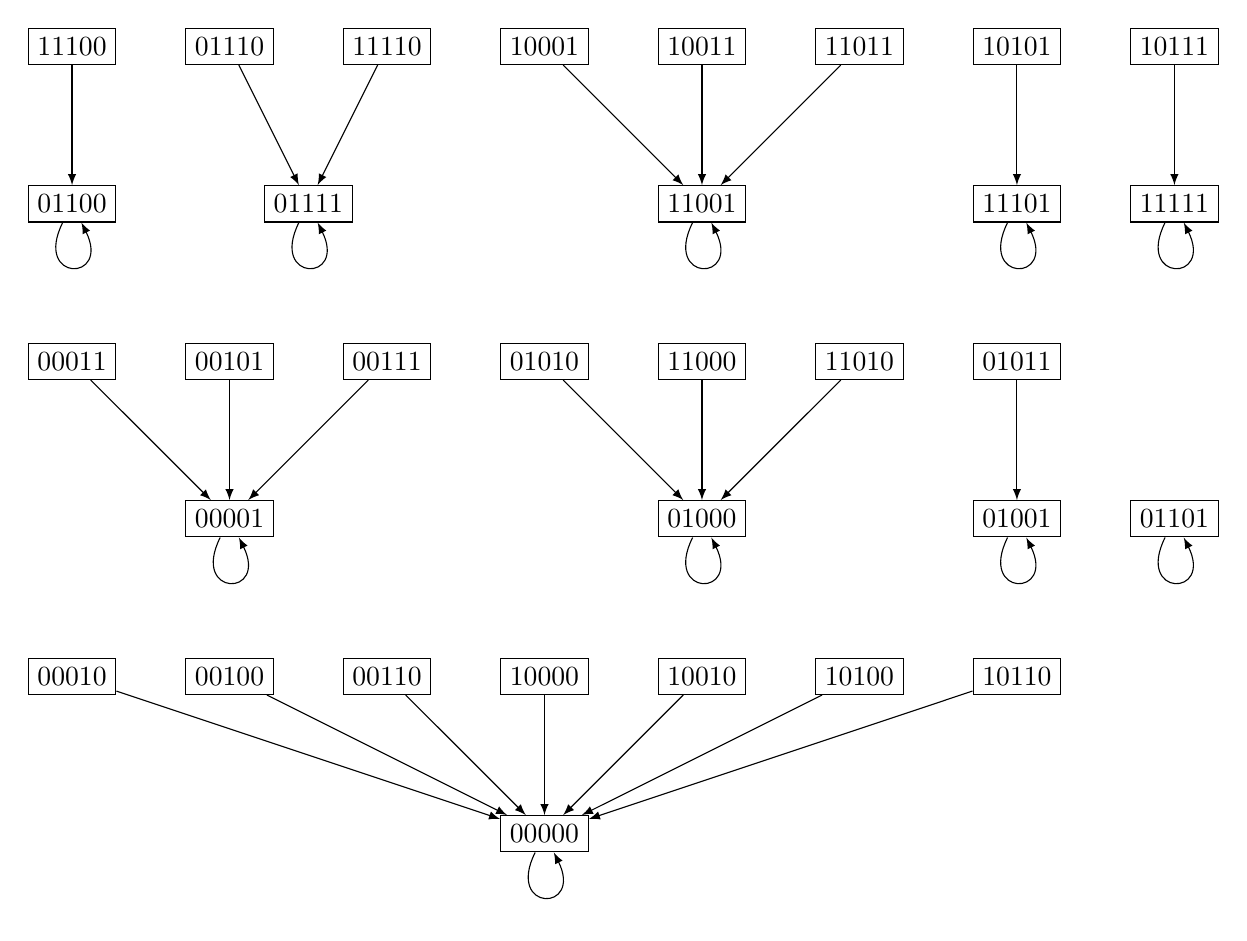
\begin{tikzpicture}
	\tikzstyle{every node}=[draw];

	\node (0) at (6,0) {00000};
	\node (1) at (2,4) {00001};
	\node (2) at (0,2) {00010};
	\node (3) at (0,6) {00011};
	\node (4) at (2,2) {00100};
	\node (5) at (2,6) {00101};
	\node (6) at (4,2) {00110};
	\node (7) at (4,6) {00111};
	
	\node (8) at (8,4) {01000};
	\node (9) at (12,4) {01001};
	\node (10) at (6,6) {01010};
	\node (11) at (12,6) {01011};
	\node (12) at (0,8) {01100};
	\node (13) at (14,4) {01101};
	\node (14) at (2,10) {01110};
	\node (15) at (3,8) {01111};
	
	\node (16) at (6,2) {10000};
	\node (17) at (6,10) {10001};
	\node (18) at (8,2) {10010};
	\node (19) at (8,10) {10011};
	\node (20) at (10,2) {10100};
	\node (21) at (12,10) {10101};
	\node (22) at (12,2) {10110};
	\node (23) at (14,10) {10111};
	
	\node (24) at (8,6) {11000};
	\node (25) at (8,8) {11001};
	\node (26) at (10,6) {11010};
	\node (27) at (10,10) {11011};
	\node (28) at (0,10) {11100};
	\node (29) at (12,8) {11101};
	\node (30) at (4,10) {11110};
	\node (31) at (14,8) {11111};

	\draw[-latex] (0) .. controls(5.5, -1) and (6.5, -1) .. (0);
	\draw[-latex] (2) -- (0);
	\draw[-latex] (4) -- (0);
	\draw[-latex] (6) -- (0);
	\draw[-latex] (16) -- (0);
	\draw[-latex] (18) -- (0);
	\draw[-latex] (20) -- (0);
	\draw[-latex] (22) -- (0);

	\draw[-latex] (1) .. controls(1.5, 3) and (2.5, 3) .. (1);
	\draw[-latex] (3) -- (1);
	\draw[-latex] (5) -- (1);
	\draw[-latex] (7) -- (1);

	\draw[-latex] (8) .. controls(7.5, 3) and (8.5, 3) .. (8);
	\draw[-latex] (24) -- (8);
	\draw[-latex] (26) -- (8);
	\draw[-latex] (10) -- (8);

	\draw[-latex] (9) .. controls(11.5, 3) and (12.5, 3) .. (9);
	\draw[-latex] (11) -- (9);

	\draw[-latex] (12) .. controls(-0.5, 7) and (0.5, 7) .. (12);
	\draw[-latex] (28) -- (12);

	\draw[-latex] (13) .. controls(13.5, 3) and (14.5, 3) .. (13);

	\draw[-latex] (15) .. controls(2.5, 7) and (3.5, 7) .. (15);
	\draw[-latex] (14) -- (15);
	\draw[-latex] (30) -- (15);

	\draw[-latex] (25) .. controls(7.5, 7) and (8.5, 7) .. (25);
	\draw[-latex] (17) -- (25);
	\draw[-latex] (19) -- (25);
	\draw[-latex] (27) -- (25);

	\draw[-latex] (29) .. controls(11.5, 7) and (12.5, 7) .. (29);
	\draw[-latex] (21) -- (29);

	\draw[-latex] (31) .. controls(13.5, 7) and (14.5, 7) .. (31);
	\draw[-latex] (23) -- (31);
\end{tikzpicture}
\caption{The dynamics of $f^\sigma$ from Example \ref{ex:schedule_vecC5}} \label{fig:schedule_vecC5}
\end{figure}	
\end{example}	



















































\section{Finite Dynamical Systems: definition and notation} \label{sec:FDS_def}

\subsection{Definition and representation of Finite Dynamical Systems} \label{sec:FDS_definition_and_representation}

A \BF{Finite Dynamical System}\index{Finite Dynamical System} (FDS) is formally defined as follows. Let $\(q\) = \{0, 1, \dots, q-1\}$ be a finite \BF{alphabet}\index{alphabet} of cardinality $q \ge 2$ and let $n$ be a positive integer. The set of all functions $f : \(q\)^n \to \(q\)^n$ is denoted as $\functions(n, q)$. Then an FDS is a function $f = (f_1,\dots,f_n) \in \functions(n,q)$. 

An element $x = (x_1, \dots, x_n)$ is called a \BF{state}\index{state}. For any $S = \{s_1, \dots, s_k\} \subseteq [n]$, we denote $x_S = (x_{s_1}, \dots, x_{s_k})$, where the order is either insignificant or clear from the context. For every $v \in [n]$, the \BF{local function}\index{function!local} $f_v : \(q\)^n \to \(q\)$ represents the update of the \BF{local state}\index{state!local} $x_v \in \(q\)$. We adopt shorthand notation for local functions that is similar to what we introduced for states, thus using $f_S$. 








%\subsection{Representing a function} \label{sec:representing_FDS}

There are numerous ways to represent the function $f \in \functions(n,q)$. 

\begin{itemize}
\item Firstly, we can give an explicit expression for each local function $f_v$. For instance, if $q=2$, we may use the logical connectives $\land, \lor, \neg$; if $q$ is a prime power, we may use the polynomial representation of $f_v$ over $\GF(q)$. 

\item Secondly, we can display $f$ as a table of inputs and outputs. 

\item Thirdly, we can represent this table as the \BF{graph} of $f$\index{graph of a function}:
\[
	\graph(f) := (\(q\)^n, \{(x, f(x)) : x \in \(q\)^n\}).
\]
It directly follows the definition of $f$ and fully characterises it.

\item Fourthly, the \BF{asynchronous graph}\index{graph of a function!asynchronous} of $f$ is
\[
	\AGraph(f) := (\(q\)^n, \{(x, x + e^v): f_v(x) > x_v\} \cup \{(x, x - e^v): f_v(x) < x_v\}).
\]
The asynchronous graph then encodes the variations of the function qualitatively. When $q = 2$, this again fully characterises $f$. However, whenever $q \ge 3$, there exist different functions with the same asynchronous graph, as seen from Figure \ref{fig:ex_asynchronous_graph}.

It is clear that the asynchronous graph of any function $f \in \functions(n,q)$ is a subgraph of $\mathrm{Grid}(n,q)$. The asynchronous graph then gives a more structured way of representing $f$ and can highlight some symmetries which are not apparent from the graph of $f$, as seen from Example \ref{ex:running_example_ch1}.
\end{itemize}


\begin{figure}[!htp]
\centering
\subfloat[$\graph(f)$]{
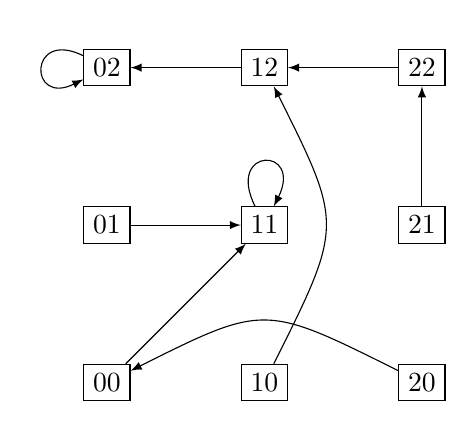
\begin{tikzpicture}
	\tikzstyle{every node}=[draw];
	
	\node (00) at (0,0) {00};
	\node (01) at (0,2) {01};
	\node (02) at (0,4) {02};
	\node (10) at (2,0) {10};
	\node (11) at (2,2) {11};
	\node (12) at (2,4) {12};
	\node (20) at (4,0) {20};
	\node (21) at (4,2) {21};
	\node (22) at (4,4) {22};

	\draw[-latex] (00) -- (11);
	\draw[-latex] (01) -- (11);
	\draw[-latex] (02) .. controls(-1, 4.5) and (-1, 3.5) .. (02);
	\draw[-latex] (10) .. controls(3, 2) .. (12);	
	\draw[-latex] (11) .. controls(1.5, 3) and (2.5, 3) .. (11);
	\draw[-latex] (12) -- (02);
	\draw[-latex] (20) .. controls(2, 1) .. (00);
	\draw[-latex] (21) -- (22);
	\draw[-latex] (22) -- (12);
\end{tikzpicture}} \hspace{1cm}
\subfloat[$\graph(g)$]{
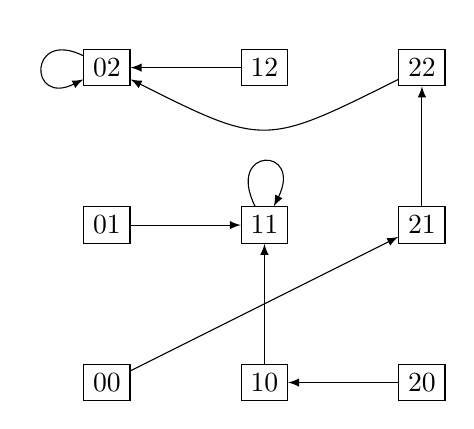
\begin{tikzpicture}
	\tikzstyle{every node}=[draw];
	
	\node (00) at (0,0) {00};
	\node (01) at (0,2) {01};
	\node (02) at (0,4) {02};
	\node (10) at (2,0) {10};
	\node (11) at (2,2) {11};
	\node (12) at (2,4) {12};
	\node (20) at (4,0) {20};
	\node (21) at (4,2) {21};
	\node (22) at (4,4) {22};

	\draw[-latex] (00) -- (21);
	\draw[-latex] (01) -- (11);
	\draw[-latex] (02) .. controls(-1, 4.5) and (-1, 3.5) .. (02);
	\draw[-latex] (10) -- (11);	
	\draw[-latex] (11) .. controls(1.5, 3) and (2.5, 3) .. (11);
	\draw[-latex] (12) -- (02);
	\draw[-latex] (20) -- (10);
	\draw[-latex] (21) -- (22);
	\draw[-latex] (22) .. controls(2, 3) .. (02);
\end{tikzpicture}} \hspace{1cm}
\subfloat[$\AGraph(f) = \AGraph(g)$]{
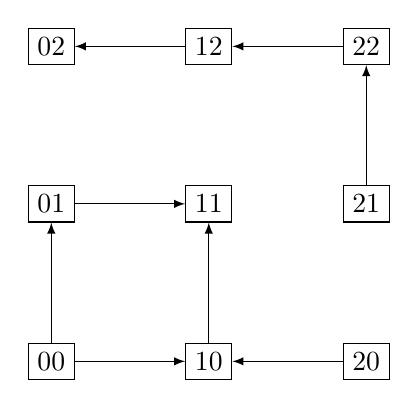
\begin{tikzpicture}
	\tikzstyle{every node}=[draw];
	
	\node (00) at (0,0) {00};
	\node (01) at (0,2) {01};
	\node (02) at (0,4) {02};
	\node (10) at (2,0) {10};
	\node (11) at (2,2) {11};
	\node (12) at (2,4) {12};
	\node (20) at (4,0) {20};
	\node (21) at (4,2) {21};
	\node (22) at (4,4) {22};

	\draw[-latex] (00) -- (01);
	\draw[-latex] (00) -- (10);
	
	\draw[-latex] (01) -- (11);
	
	\draw[-latex] (10) -- (11);
	
	\draw[-latex] (12) -- (02);
	
	\draw[-latex] (20) -- (10);
	
	\draw[-latex] (21) -- (22);
	
	\draw[-latex] (22) -- (12);
\end{tikzpicture}}
\caption{Two different functions with the same asynchronous graph} \label{fig:ex_asynchronous_graph}
\end{figure}




\begin{example}\label{ex:running_example_ch1}[Running example for Section \ref{sec:FDS_def}]
Here is a function $f \in \functions(4, 2)$, given in four equivalent representations.

Firstly, the local functions are expressed (using $\GF(2)$) by
\begin{align*}
	f_1(x) &= x_3 (x_2 + x_4 + 1)\\
	f_2(x) &= x_1 (x_3 + 1)\\
	f_3(x) &= x_2 (x_1 + 1)\\
	f_4(x) &= x_4 + x_1 x_2 x_3.
\end{align*}

Secondly, the table of $f$ is as follows.\\
~\\
\begin{tabular}{c|c}
	$x$ & $f(x)$\\
	\hline
	$0000$ & $0000$\\
	$0001$ & $0001$\\
	$0010$ & $1000$\\
	$0011$ & $0001$\\
	$0100$ & $0010$\\
	$0101$ & $0011$\\
	$0110$ & $0010$\\
	$0111$ & $1011$\\
	$1000$ & $0100$\\
	$1001$ & $0101$\\
	$1010$ & $1000$\\
	$1011$ & $0001$\\
	$1100$ & $0100$\\
	$1101$ & $0101$\\
	$1110$ & $0001$\\
	$1111$ & $1000$
\end{tabular}

Thirdly, the graph $\graph(f)$ of $f$ is depicted below.\\
~\\
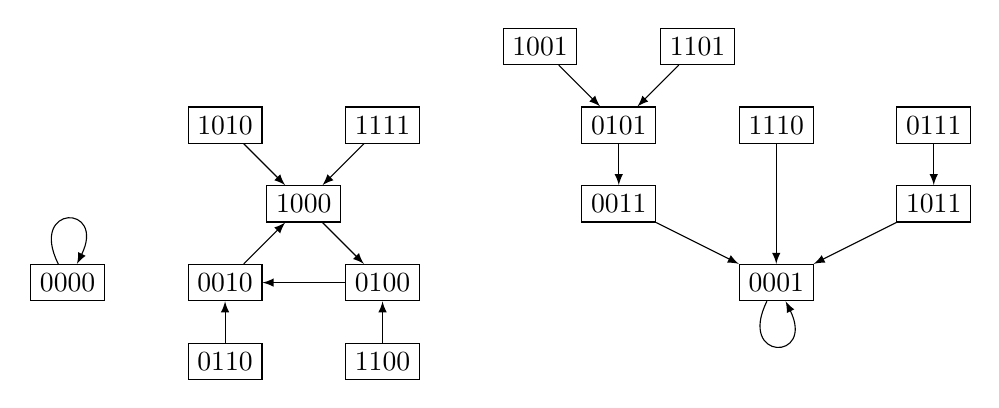
\begin{tikzpicture}
	\tikzstyle{every node}=[draw];
	
	\node (0000) at (0,0) {$0000$};
	\draw[-latex] (0000) .. controls(-0.5, 1) and (0.5, 1) .. (0000);
	
	\node (0110) at (2,-1) {$0110$};
	\node (1100) at (4,-1) {$1100$};
	
	\node (0010) at (2,0) {$0010$};
	\node (0100) at (4,0) {$0100$};

	\node (1000) at (3,1) {$1000$};
	\node (1010) at (2,2) {$1010$};
	\node (1111) at (4,2) {$1111$};
	
	\draw[-latex] (0110) -- (0010);
	\draw[-latex] (1010) -- (1000);
	\draw[-latex] (1111) -- (1000);
	\draw[-latex] (1100) -- (0100);
	\draw[-latex] (0100) -- (0010);
	\draw[-latex] (0010) -- (1000);
	\draw[-latex] (1000) -- (0100);
	
	\node (1001) at (6,3) {$1001$};
	\node (1101) at (8,3) {$1101$};
	\node (0101) at (7,2) {$0101$};
	\node (0011) at (7,1) {$0011$};
	\node (0001) at (9,0) {$0001$};
	\node (1011) at (11,1) {$1011$};
	\node (0111) at (11,2) {$0111$};
	\node (1110) at (9,2) {$1110$};

	\draw[-latex] (1001) -- (0101);
	\draw[-latex] (1101) -- (0101);
	\draw[-latex] (0101) -- (0011);
	\draw[-latex] (0011) -- (0001);
	\draw[-latex] (0001) .. controls(8.5, -1) and (9.5, -1) .. (0001);
	\draw[-latex] (1011) -- (0001);
	\draw[-latex] (0111) -- (1011);
	\draw[-latex] (1110) -- (0001);
\end{tikzpicture}


Fourthly, the asynchronous graph $\AGraph(f)$ of $f$ is the following:\\
~\\
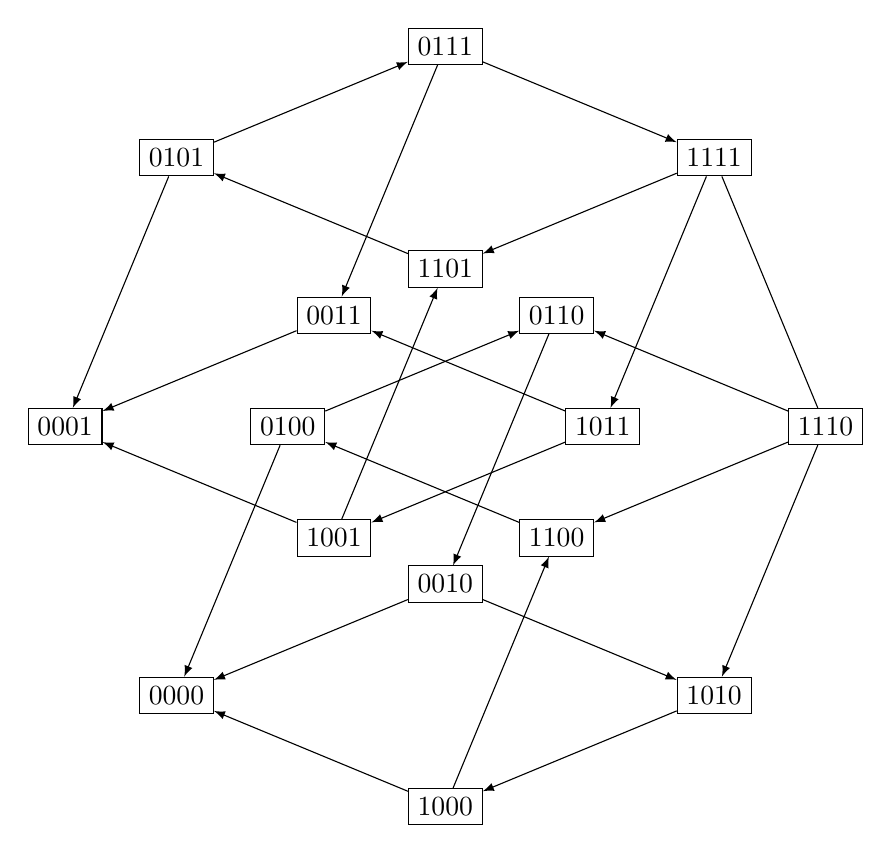
\begin{tikzpicture}
\tikzstyle{every node}=[draw];
\pgfmathparse{2}
\node (1011) at (0:\pgfmathresult){$1011$};
\node (0110) at (45:\pgfmathresult){$0110$};
\node (1101) at (90:\pgfmathresult){$1101$};
\node (0011) at (135:\pgfmathresult){$0011$};
\node (0100) at (180:\pgfmathresult){$0100$};
\node (1001) at (225:\pgfmathresult){$1001$};
\node (0010) at (270:\pgfmathresult){$0010$};
\node (1100) at (315:\pgfmathresult){$1100$};
\pgfmathparse{\pgfmathresult*sqrt(2*cos(45)*cos(45)+2*(1+sin(45))*(1+sin(45))-1)}
\node (1110) at (0:\pgfmathresult){$1110$};
\node (1111) at (45:\pgfmathresult){$1111$};
\node (0111) at (90:\pgfmathresult){$0111$};
\node (0101) at (135:\pgfmathresult){$0101$};
\node (0001) at (180:\pgfmathresult){$0001$};
\node (0000) at (225:\pgfmathresult){$0000$};
\node (1000) at (270:\pgfmathresult){$1000$};
\node (1010) at (315:\pgfmathresult){$1010$};
\path[-latex]
(1100) edge (0100)
(0110) edge (0010)
(1010) edge (1000)
(1111) edge (1011)
(1111) edge (1101)
(0100) edge (0000)
(0100) edge (0110)
(0010) edge (1010)
(0010) edge (0000)
(1000) edge (1100)
(1000) edge (0000)
(1001) edge (0001)
(1001) edge (1101)
(1101) edge (0101)
(0101) edge (0001)
(0101) edge (0111)
(0011) edge (0001)
(0111) edge (1111)
(0111) edge (0011)
(1011) edge (0011)
(1011) edge (1001)
(1110) edge (0110)
(1110) edge (1010)
(1110) edge (1100)
;
\draw (1111) -- (1110);
\end{tikzpicture}
\end{example}
%%%%%%%%%%%%%%%%%%






\subsection{Interaction graphs} \label{sec:interaction_graphs}

The dependencies amongst entities are encoded qualitatively in the (signed) interaction graph of $f$. They represent the architecture of the network.

Formally, the \BF{interaction graph} \label{graph!interaction} of $f$, denoted as $\IG(f)$, has vertex set $[n]$ and $uv$ is an arc in $\IG(f)$ if and only if $f_v$ depends essentially on $x_u$, i.e. there exist $a,b \in \(q\)^n$ that only differ by $a_u \ne b_u$ such that $f_v(a) \ne f_v(b)$. 
 
We can refine this as follows. The signed graph $\SIG(f)$, referred to as the \BF{signed interaction graph}\index{graph!signed interaction} of $f$ is defined by: the vertex set is $[n]$; and for all $u,v\in [n]$, there exists a positive arc $(u, v, 1) \in \SIG(f)$ if and only if there exist $a, b \in \(q\)^n$ such that $a_u < b_u$, $a_w = b_w$ for all $w \ne u$ and $f_v(a) < f_v(b)$; there exists a negative arc $(u, v, -1) \in \SIG(f)$ if and only if there exist $a, b \in \(q\)^n$ such that $a_u < b_u$, $a_w = b_w$ for all $w \ne u$ and $f_v(a) > f_v(b)$.

The interaction graph of $f$ is then the underlying graph of the signed interaction graph of $f$: 
\[
	\IG(f) = |\SIG(f)|.
\]

We denote the set of all functions $f \in \functions(n,q)$ with interaction graph equal to (a subgraph of) a graph $D$ as 
\begin{align*} 
	\functions(D,q) &= \{f \in \functions(n,q) : \IG(f) \subseteq D \},\\
	\functions[D,q] &= \{f \in \functions(n,q) : \IG(f) = D \}.
\end{align*}
For signed interaction graphs, we similarly define
\begin{align*}
	\functions(G,q) &= \{f \in \functions(n,q) : \SIG(f) \subseteq G \},\\
	\functions[G,q] &= \{f \in \functions(n,q) : \SIG(f) = G \}.
\end{align*}

\begin{example}[Continued from Example \ref{ex:running_example_ch1}]\label{ex:running_IG}
The interaction graph and the signed interaction graph of $f$ are given below.\\
~\\
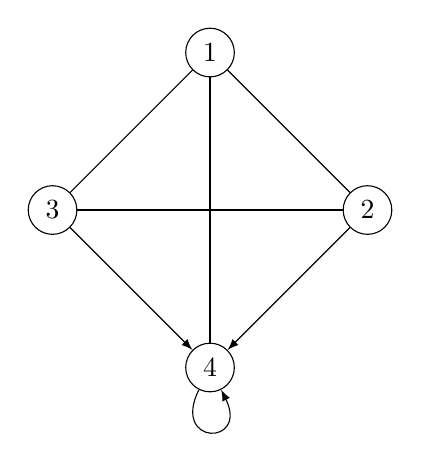
\begin{tikzpicture}	
	\node[draw, shape = circle] (1) at (2,2) {$1$};
	\node[draw, shape = circle] (2) at (4,0) {$2$};
	\node[draw, shape = circle] (3) at (0,0) {$3$};
	\node[draw, shape = circle] (4) at (2,-2) {$4$};
	
	\draw (1) -- (2);
	\draw (1) -- (3);
	\draw (1) -- (4);
	\draw (2) -- (3);
	\draw[-latex] (2) -- (4);
	\draw[-latex] (3) -- (4);
	\draw[-latex] (4) .. controls(1.5, -3) and (2.5, -3) .. (4);
\end{tikzpicture} \hspace{1cm}
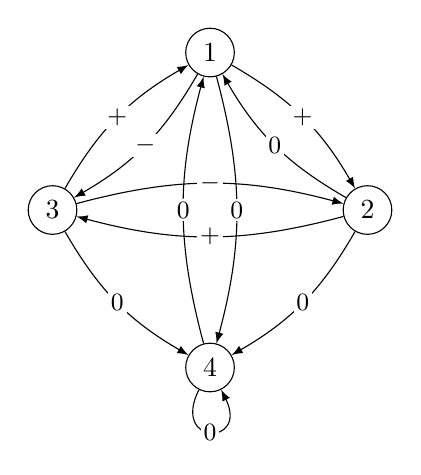
\begin{tikzpicture}
	\node[draw, shape = circle] (1) at (2,2) {$1$};
	\node[draw, shape = circle] (2) at (4,0) {$2$};
	\node[draw, shape = circle] (3) at (0,0) {$3$};
	\node[draw, shape = circle] (4) at (2,-2) {$4$};
	
	\draw[-latex] (2) to [bend left=15] node[midway,fill=white,inner sep=1] {\small $0$} (1);
	\draw[-latex] (3) to [bend left=15] node[midway,fill=white,inner sep=1] {\small $+$} (1);
	\draw[-latex] (4) to [bend left=15] node[midway,fill=white,inner sep=1] {\small $0$} (1);
	\draw[-latex] (1) to [bend left=15] node[midway,fill=white,inner sep=1] {\small $+$} (2);
	\draw[-latex] (3) to [bend left=15] node[midway,fill=white,inner sep=1] {\small $-$} (2);
	\draw[-latex] (1) to [bend left=15] node[midway,fill=white,inner sep=1] {\small $-$} (3);
	\draw[-latex] (2) to [bend left=15] node[midway,fill=white,inner sep=1] {\small $+$} (3);
	\draw[-latex] (1) to [bend left=15] node[midway,fill=white,inner sep=1] {\small $0$} (4);
	\draw[-latex] (2) to [bend left=15] node[midway,fill=white,inner sep=1] {\small $0$} (4);
	\draw[-latex] (3) to [bend right=15] node[midway,fill=white,inner sep=1] {\small $0$} (4);
	\draw[-latex] (4) .. controls(1.5, -3) and (2.5, -3) .. (4) node[midway,fill=white,inner sep=1] {\small $0$} (4);
\end{tikzpicture}
\end{example}






\subsection{Dynamical properties} \label{sec:dynamical_properties}

Let $f \in \functions(n,q)$ and $x \in \(q\)^n$. 

We say that $x$ is an \BF{image}\index{image} of $f$ if there is $y \in \(q\)^n$ such that $f(y) = y$. The image of $f$ is the set $\image(f)$ of all its images; the rank of $f$ is the number of images of $f$: $\rank(f) = |\image(f)|$. The \BF{kernel}\index{kernel} of $f$ is the partition of $\(q\)^n$ into pre-images of $f$: 
\[
	\ker(f) = \{f^{-1}(a) : a \in \image(f)\},
\]
where $f^{-1}(a) = \{ x \in \(q\)^n : f(x) = a \}$ (this does not mean that $f$ is invertible!).

Moreover, $x$ is a \BF{periodic point}\index{periodic point} of $f$ if here exists $p \ge 1$ such that $f^p(x) = x$; $x$ is \BF{transient}\index{state!transient} otherwise. The set of periodic points of $f$ is denoted $\periodic(f)$ and its cardinality is the \BF{periodic rank}\index{rank!periodic} of $f$: $\periodicRank(f) := |\periodic(f)|$.

A \BF{limit cycle}\index{cycle!limit} is a cycle in $\graph(f)$. Clearly, the limit cycles form a partition of $\periodic(f)$. Note that the limit cycles of $f$ are exactly the terminal components of its graph $\graph(f)$. Conversely, an \BF{attractor}\index{attractor} is a terminal component of $\AGraph(f)$. The \BF{period}\index{period} of $f$ is the least common multiple of all lengths of its limit cycles. The \BF{length}\index{length} of $f$ is the smallest $k$ such that for all $x \in \(q\)^n$, $f^k(x)$ is periodic. Then, if $p$ is the period of $f$, $f^{k+p} = f^k$ and $p$ and $k$ are minimal. 

Finally, $x$ is a \BF{fixed point}\index{fixed point} of $f$ if $f(x) = x$. The set of fixed points of $f$ is denoted as $\Fix(f)$. Clearly, we have
\[
	\Fix(f) \subseteq \periodic(f) \subseteq \image(f).
\]

\begin{example}[Continued from Examples \ref{ex:running_example_ch1} and \ref{ex:running_IG}]
The dynamical properties introduced above can be easily determined for $f$. 

The fixed points of $f$ are $0000$ and $0001$; its periodic points are $0000, 0001, 1000, 0100, 0010$; its transient states are $1100, 0110, 1010, 1111, 1001, 1101, 0101, 0011, 0111, 1011, 1110$. (All these are easily seen from the graph of $f$.)

The attractors of $f$ are its fixed points $0000$ and $0001$ and a limit cycle of length three $1000, 0100, 0010$. The only asynchronous attractors of $f$ are its fixed points. We remark that it is difficult to determine the asynchronous attractors without using the asynchronous graph of $f$.

The period of $f$ is three; its length is three also (the longest paths to reach an attractor are $1001, 0101, 0011, 0001$ and $1101, 0101, 0011, 0001$).

The rank of $f$ is equal to nine. Its periodic rank is equal to five. Its kernel is given by
$\{0000\},$ $\{0010, 1010, 1111\}, \{1000, 1100\}, \{0100, 0110\},$ $\{0001, 0011, 1011, 1110\}, \{1001, 1101\}, \{0101\}, \{0111\}.$
\end{example}





\subsection{Schedules} \label{sec:schedules}

So far, we considered the function $f$ only, and we were focusing on the transition from $x$ to $f(x)$, possibly repeated multiple times: $x, f(x), f^2(x), \dots$. In other words, we assume that the states $x_v$ all perform their updates at the same time. However, in many situations--either arising from applications or for theoretical considerations--, we need to consider the case where these local updates are performed asynchronously. We will represent the different updates at each time step by a \BF{schedule}\index{schedule}. 

For $n \ge 1$, let $2_+^{[n]}$ denote the set of all non-empty subsets of $[n]$ and $(2_+^{[n]})^* = \bigcup_{T=0}^\infty (2_+^{[n]})^T$ denote the set of finite sequences of non-empty subsets of $[n]$. Then an element $\sigma$ of $(2_+^{[n]})^*$ is referred to as a schedule. We have $\sigma = (\sigma_1, \dots, \sigma_T)$, where $\sigma_t \subseteq [n]$ represents which local states $x_v$ get updated to $f_v(x)$ at time $t$. (When $T=0$, $\sigma$ is the empty schedule, which we shall denote as $\epsilon$.)

We introduce some terminology for schedules. Firstly, if $\sigma = (\sigma_1, \dots, \sigma_T)$, then $T$ is the \BF{length} \label{schedule!length of a} of $\sigma$. next, for any $S \subseteq \{1, \dots, n\}$, we denote the update of the local states in $S$ according to $f$ as $f^{(S)}$, i.e. $f^{(S)} \in \functions(n,q)$ where
\[
	f^{(S)}_v(x) = \begin{cases}
		f_v(x) &\text{if } v \in S\\
		x_v &\text{otherwise}.
	\end{cases}
\]
Alternatively, we have $f^{(S)}_S = f_S$ and $f^{(S)}_{- S} = \id_{- S}$. 

We denote the application of $f$ with the schedule of $\sigma$ as $f^\sigma$, where
\[
	f^\sigma = f^{(\sigma_T)} \circ \cdots \circ f^{(\sigma_1)}.
\]
In particular, if $\sigma^k = ([n], \dots, [n])$ (with length $k$), then $f^{\sigma^k} = f^k$.

Let us make a few remarks on notation. Firstly, in a sense, our notation $f^{(S)}$ identifies a set $S \subseteq [n]$ with the corresponding schedule $(S)$ of length one. Secondly, as usual, we identify a singleton $\{v\}$ with its element $v$, and we denote $f^{(v)} = f^{(\{v\})}$. Any update of the form $f^{(v)}$ is referred to as an \BF{instruction}\index{instruction}. Thirdly, if $f$ is an FDS and $i$ an integer, then there may be a confusion between $f^i = f \circ \dots \circ f$ and $f^i$ being the member of a family $f^1, \dots, f^k$ of functions. We will not try to differentiate the two, instead the context should make it clear which meaning we give to $f^i$.


\begin{example}[Continuation of Example \ref{ex:running_example_ch1}] \label{ex:running_schedule}
We give two examples of what $f^\sigma$ looks like for some choices of $\sigma$. First, let $\rho = (\{1\},\{2\},\{3\},\{4\})$, then
\begin{align*}
	f_1^\rho(x) &= x_3 (x_2 + x_4 + 1)\\
	f_2^\rho(x) &= f_1^\rho(x) (x_3 + 1) = 0\\
	f_3^\rho(x) &= f_2^\rho(x) (f_1^\rho(x) + 1) = 0\\
	f_4^\rho(x) &= x_4 + f_1^\rho(x) f_2^\rho(x) f_3^\rho(x) = x_4.
\end{align*}
That is a dramatic change indeed!

Now, let us consider the schedule $\tau = (\{1,2,3\},\{4\})$. We have
\begin{align*}
	f_1^\tau(x) &= f_1(x) = x_3 (x_2 + x_4 + 1)\\
	f_2^\tau(x) &= f_2(x) = x_1 (x_3 + 1)\\
	f_3^\tau(x) &= f_3(x) = x_2 (x_1 + 1)\\
	f_4^\tau(x) &= x_4 + f_1(x)f_2(x)f_3(x) = x_4.
\end{align*}
This still affects the fourth local function.
\end{example}


We now review some special classes of schedules. Let $\sigma = (\sigma_1, \dots, \sigma_T)$ be a schedule of length $T$. The schedule is \BF{complete}\index{schedule!complete} if $\bigcup_{t=1}^T \sigma_t = [n]$. In other words, in a complete schedule, every local state is updated at least once. In particular, $\sigma$ is \BF{block-parallel}\index{schedule!block-parallel} if $\sigma_t = P_t$ for all $1 \le t \le T$ for some partition $P = \{P_1, \dots, P_T\}$ of $[n]$. In other words, in a block-parallel schedule, every local state is updated exactly once. We will focus on the two extreme kinds of block-parallel schedules. First, $\sigma$ is \BF{parallel}\index{schedule!parallel} if $T = 1$ and $\sigma_1 = [n]$; in the parallel schedule, $x$ is updated to $f(x)$. Second, $\sigma$ is \BF{Gauss-Seidel}\index{schedule!gauss-Seidel} if $T = n$ and $\sigma_t = \pi(t)$ for all $1 \le t \le n$ for some permutation $\pi$ of $[n]$. Note that in \cite{Rob95}, only the case $\pi = \id$ is viewed as Gauss-Seidel; this is at no loss of generality. Finally, $\sigma$ is \BF{sequential} if $|\sigma_t| = 1$ for all $1 \le t \le T$. Thus a schedule is Gauss-Seidel if and only if it is sequential and block-parallel.










\section{Exercises} \label{sec:ch1_exercises}

\begin{exercises}

%%%% Sanity checks


\item Sanity check part one. Verify that for an FDS $f \in \functions(n,q)$, the following are equivalent.
\begin{exercises}
	\item $f$ is bijective;
	
	\item $f$ is surjective;
	
	\item $f$ is injective;
	
	\item $f$ is a permutation of $\(q\)^n$;
	
	\item $f$ has rank $q^n$;
	
	\item the kernel of $f$ is the equality partition $\{ \{x\} : x \in \(q\)^n \}$  (with $q^n$ parts);
	
	\item $f$ has $q^n$ periodic points;
	
	\item $f$ has length zero;
	
	\item $\periodic(f) = \image(f)$;
	
	\item all the connected components of $\graph(f)$ are strong;
	
	\item $\graph(f)$ has no sources;
	
	\item there exists $g \in \functions(n, q)$ such that $g \circ f = \id$;
	
	\item $f^p = \id$, where $p$ is the period of $f$.
\end{exercises}


\item Sanity check part two. Verify that for an FDS $f \in \functions(n,q)$, the following are equivalent.
\begin{exercises}
	\item $f$ is idempotent, i.e. $f^2 = f$;

	\item $f$ has length one and period one;
	
	\item all images of $f$ are fixed points;
	
	\item $\graph(f)$ does not have any path of length two;
		
	\item $x \in f^{-1}(x)$ for all $x \in \image(f)$.
\end{exercises}


\item Sanity check part three. Verify that for an FDS $f \in \functions(n,q)$, the following are equivalent.
\begin{exercises}
	\item $f$ is constant;
	
	\item $f$ has rank $1$;
	
	\item the kernel of $f$ is the universal partition $\{ \(q\)^n \}$ (with one part);
	
	\item $f$ has exactly one periodic point and length one;
	
	\item $f$ is idempotent and $\graph(f)$ is connected;
	
	\item $f \circ g = f$ for all $g \in \functions(n, q)$.
\end{exercises}



\item \label{exerc:sanity_check_cyclic_derangement} Sanity check part four. Verify that for an FDS $f \in \functions(n,q)$, the following are equivalent.
\begin{exercises}
	\item $f$ is the successor function of some ordering of $\(q\)^n$, i.e. there exists an ordering $x^0, \dots, x^{q^n-1}$ of $\(q\)^n$ and $f(x^i) = x^{i+1 \mod q^n}$ for all $i$;

	\item $f$ is a cyclic derangement, i.e. $f = (x^0 \espace x^1 \espace \dots \espace x^{q^n-1})$;
	
	\item $f$ is a permutation of period $q^n$;
	
	\item $X \subseteq \(q\)^n$ satisfies $f(X) \subseteq X$ only if $X = \emptyset$ or $X = \(q\)^n$;
	
	\item $\graph(f)$ is a cycle;
	
	\item $\graph(f)$ is strong;
	
	\item $f$ is a permutation and $\graph(f)$ is connected.
\end{exercises}



%%%% Hat game example

\item Let $f$ be the function in the hat game example of Section \ref{sec:hat_game_example} for $n=3$ (i.e. $f \in \functions(3,3)$). Draw the signed interaction graph of $f$ and determine the rank, periodic rank, length and period of $f$.



%%%% Rumour spreading example


\item \label{exerc:rumour} Prove the following claims about the function $f$ from Section \ref{sec:rumour}:
\begin{enumerate}
	\item Verify that $1$ is a fixed point of $f$.

	\item Find $x$ of Hamming weight two such that $f^p(x) = 1$ for some $p \ge 1$.
	
	\item Prove that for any schedule $\sigma$ and any $v \in \{1, \dots, 7\}$, $f^\sigma(e^v) \ne 1$.
\end{enumerate}

\item Let $f$ be the function from Section \ref{sec:rumour}. Draw the signed interaction graphs of $f$, $f^\rho$, $f^\sigma$ and $f^\tau$, where $\rho = (\{1,2\}, \{1, \dots, 7\})$, $\sigma = (\{1,2,3\}, \{4, 5, 6, 7\})$ and $\tau = (\{5,6,7\}, \{3,4\}, \{1,2\})$.


%%%%% Section 1.2 example

\item \label{exerc:number_fixed_points_example} We will determine the asymptotic behaviour of the number of fixed points in Example \ref{ex:3_vecC5}. For all $q \ge 2$, let $k^q \in \functions(5, q)$ defined by the same local functions as $k$, Hence $k^2 = f$ from Example \ref{ex:monotone_vecC5} and $k^3 = k$. Moreover, let $T$ be the set of fixed points $x$ of $k^5$ such that $x_1, \dots, x_5$ are all distinct.
\begin{exercises}
	\item Prove that $|T| = 8$.
	
	\item Prove that for $q \ge 5$,
	\[
		|\Fix(k^q)| = \binom{q}{5} |T| + O(q^4).
	\]
	
	\item Conclude that $|\Fix(k^q)| = \frac{1}{15} q^5 + O(q^4).$
\end{exercises}

\item Let $k^q$ be defined as in Exercise \ref{exerc:number_fixed_points_example}. Show that the length of $k^q$ is no more than $5! + 4! + 3! + 2! + 1! - 1 = 152$ for all $q$.




%%%%% FDS: interaction graphs



\item Let us compare the number of functions in $\functions(D,q)$ to that in $\functions[D,q]$.
\begin{exercises}
	\item Give a formula for $|\functions(D,q)|$.
	
	\item Give a formula for $|\functions[D,q]|$ based on the principle of inclusion-exclusion.
	
	\item Show that for any $D$, there exists $A_D$ such that
	\[
		|\functions[D, q]| = |\functions(D, q)| \left( 1 - A_D q^{-1} + O(q^{-2}) \right),
	\]
	and hence
	\[
		\lim_{q \to \infty} \frac{|\functions[D, q]|}{|\functions(D, q)|} = 1.
	\]
\end{exercises}

\item Determine the number of FDSs in $\functions(n, q)$ with rank $r$, for all $1 \le r \le q^n$. What is the average rank of an FDS in $\functions(n, q)$?

\item \label{exerc:number_FDS_k_with_fixed_points} Determine the number of FDSs in $\functions(n, q)$ with $k$ fixed points, for all $0 \le k \le q^n$. What is the average number of fixed points of an FDS in $\functions(n, q)$?


\item Let $f \in \functions(n,2)$ and $v \in [n]$. Prove that the corresponding instruction $f^{(v)}$ is a permutation if and only if $f_v(x) = x_v + g(x_{- v})$ for some $g : \(2\)^{n-1} \to \(2\)$.

\item For any $n \ge 2$ and $q$, exhibit an FDS $f \in \functions(n,q)$ such that $f$ is a permutation, yet $f^{(S)}$ is not a permutation for any nonempty $S \subset [n]$.

\item Prove that if $f \in \functions(n,q)$ is a bijection, then all its local functions are balanced, i.e. for any $v \in [n]$ and $a \in \(q\)$, $|f_v^{-1}(a)| = q^{n-1}$. Show that the converse does not hold.



%\item Show that a signed graph $G$ on $n$ vertices is the signed interaction graph of some FDS $f \in \functions(n,2)$ if and only if there is no $v$ such that $\dIn(v; G) = \dInZero(v; G) = 1$. Conversely, prove that for any $G$ and any $q \ge 3$, there exists $f \in \functions[G, q]$.

\item Linear functions are almost never unate.
\begin{exercises}
	\item Characterise the linear functions $\phi: \GF(q) \to \GF(q)$ which are unate (for any possible linear order of $\GF(q)$).
	
	\item Prove that, no matter how $\GF(q)$ is linearly ordered, any linear function $\phi : \GF(q)^n \to \GF(q)$ depending essentially on at least two variables is not unate.
\end{exercises}

\item \label{exerc:increasing} Say that an FDS $f \in \functions(n,q)$ is \BF{increasing}\index{function!increasing} if $f(x) \ge x$ for all $x \in \(q\)^n$. 
\begin{exercises}
	\item Prove that $D$ is the interaction graph of an increasing FDS if and only if for all $v$, either $v$  is a source or $v$ has a loop.

	\item Classify the signed graphs $G$ such that $G$ is the signed interaction graph of some increasing function.
\end{exercises}




%%%%% Asynchronous graphs


\item Let us prove that there is no counterpart of Exercise \ref{exerc:sanity_check_cyclic_derangement} for the asynchronous graph. More precisely, for any $n$ and $q$, give an example of:
\begin{exercises}
	\item an FDS $f \in \functions(n,q)$ such that $\AGraph(f)$ is strong and $f$ is not a permutation;
	
	\item an FDS $g \in \functions(n,q)$ such that $\AGraph(g)$ is not strong and $g$ is a permutation.
\end{exercises}



\item Exhibit $f$ and $g$ such that $\IG(f) \ne \IG(g)$ and $\AGraph(f) = \AGraph(g)$.

\item Characterise the graphs $\Sigma$ such that there exists a unique $f \in \functions(n,q)$ with $\AGraph(f) = \Sigma$. For a given $n$ and $q$, how many such graphs $\Sigma$ are there?

\item For $f \in \functions(n,q)$, let
\[
	\AGraph'(f) = (\(q\)^n, \{ (x, x + (f_v(x) - x_v) e^v) \}).
\]
Show that $\AGraph'(f)$ fully determines $f$ and that $\AGraph'(f) = \AGraph(f)$ if $q=2$.




%%%% Misc


\item Give the other three representations, the interaction graphs and the signed interaction graphs, and determine the dynamical properties defined in Section \ref{sec:dynamical_properties} for $f^\rho$ and $f^\tau$ in Example \ref{ex:running_schedule}.




\item Let $f \in \functions(n,n)$ be defined as $f_v(x) = v - \sum_{v \in [n]} x_v$ for all $v$. Determine the length, period and set of fixed points of $f$.



\item \label{exerc:successor_lexicographic} Let $f \in \functions(n,2)$ be the successor function of the lexicographic order. More precisely, for any $x \in \(2\)^n$, let $\hat{x} = \sum_{i=1}^n 2^{i-1} x_i \in \N$ be its lexicographic index, then $f(x) = y$ where $\hat{y} = \hat{x} + 1 \mod 2^n$.
\begin{exercises}
	\item Describe the local functions $f_v$ of $f$ and determine the (signed) interaction graph of $f$.
	
	\item Draw $\graph(f)$ and $\AGraph(f)$ for $n = 2$ and $n=3$.
	
	\item Describe the local functions of $f^\sigma$ and $f^\tau$, where $\sigma = (1, \dots, n)$ and $\tau = (n, n-1, \dots, 1)$. Verify that neither has any fixed points.
	
	\item Repeat the three items above for the successor function of the canonical Gray code (see Section \ref{sec:Hamming_metric}).
\end{exercises}




\item A function $f \in \functions(n,q)$ is \BF{affine}\index{function!affine} if $f(x) = x{\bf M} + a$ for some matrix ${\bf M} \in \GF(q)^{n \times n}$ and some state $a \in \(q\)^n$. 
\begin{exercises}
	\item Show that $\ker(f)$ is balanced.
	
	\item Show that $f$ is a permutation if and only if ${\bf M}$ is nonsingular. 
\end{exercises}

\item Prove the following relations between the rank and the periodic rank of $f \in \functions(n,q)$:
\[
	\periodicRank(f) = \lim_{k \to \infty} \rank(f^k) = \min_{k \ge 1} \rank(f^k) = \rank(f^{q^n - 1}).
\]


\item This exercise is about estimating the number $a_n$ of functions in $\functions(n,2)$ with an acyclic interaction graph. 
\begin{exercises}
	\item Let $T_n$ be the transitive tournament, with an arc $ij$ if and only if $i < j$. Determine $|\functions(T_n,2)|$.
	
	\item Let $b_k$ be the number of Boolean functions $\{0,1\}^k \to \{0,1\}$ which depend essentially on all $k$ variables. Give a lower bound on $b_k$ from which you can infer that $|\functions[T_n, 2]| \ge 2^{2^n - O(n)}$.
	
	\item Conclude that
	$
		a_n = n!2^{2^n - O(n)}.
	$
\end{exercises}

\end{exercises}













\part{Fixed points} \label{part:fixed_points}

\chapter{Fixed points for a given interaction graph} \label{ch:fixed_points_unsigned}

The interaction graph is arguably the main property of a finite dynamical system. In different contexts, the interaction graph is known--or at least well approximated--, while the actual local functions are not. One main problem of research on finite dynamical systems is then to predict their dynamics according to their interaction graphs. 

Among the many dynamical properties that can be studied, fixed points are crucial because they represent stable states. For instance, in the context of gene networks, they correspond to stable patterns of gene expression at the basis of particular biological processes. As such, they are arguably the property which has been the most thoroughly studied. The study of the number of fixed points and its maximisation in particular is the subject of a stream of work, e.g. in \cite{Rob80,ADG04,Rii06,Rii07,GR11,CM11,GRF16}. The aim of this chapter is to introduce some of the  main results and ideas in that area; we will dive deeper in the subject in Chapters \ref{ch:optimality_feedback} and \ref{ch:advanced_guessing}.



\section{Generalities} \label{sec:fixed_points_generalities}


A \BF{fixed point} \label{fixed point} of $f \in \functions(n,q)$ is a state $x \in \(q\)^n$ such that $f(x) = x$. We denote the set of fixed points of $f$ by 
\[
	\Fix(f) := \{ x \in \(q\)^n : f(x) = x \}.
\]

%The set of fixed points is equal for a large number of schedules (see \cite[Proposition 2.1]{Rob95} and \cite[Proposition 4.11]{MR08} for limited versions of the following theorem). In the following, $f$ always denotes a transformation of $\(q\)^n$.


The first main property about fixed points concerns FDSs with acyclic interaction graphs. This property was first proved by Robert in \cite{Rob80} (see also \cite{Rob86,Rob95}).

\begin{theorem}[Robert's theorem] \label{th:fixed_points_acyclic}
If $\IG(f)$ is acyclic, then $f$ has exactly one fixed point $c$; moreover, for any $x \in \(q\)^n$, $f^n(x) = c$.
\end{theorem}


\begin{proof}[Proof]
Sort the vertices in topological order. Then for any $x \in \(q\)^n$,
\begin{align*}
	f_1(x) &= c_1,\\
	f_2^2(x) &= f_2(c_1) = c_2\\
	&\vdots\\
	f_n^n(x) &= f_n(c_1, \cdots, c_{n-1}) = c_n.
\end{align*}
\end{proof}


For general interaction graphs, the situation is a lot more complex. We are then interested in the number of fixed points of FDSs with a given interaction graph. The minimum number is determined below. This is an unpublished result of Aracena and Salinas.


\begin{proposition} \label{prop:no_fixed_points_cyclic}
If $D$ is not acyclic, then for any $q$, there exists $f \in \functions[D,q]$ with no fixed points.
\end{proposition}

\begin{proof}
For any $x \in \(q\)^n$, let $\tilde x \in \(2\)^n$ be defined as $\tilde x_v = \min\{1, x_v\}$ for all $v \in [n]$. Then let $C$ be the first non-trivial strong component of $D$ according to the topological order of its strong component graph, let $I$ be a minimum feedback vertex set of $C$ and let $J = C \setminus I$. Consider $f \in \functions[D,q]$ defined by 
\[
	f_v(x) = \bigwedge_{u \in \NIn(v) \setminus I} \tilde x_u \land \bigwedge_{i \in \NIn(v) \cap I} \neg \tilde x_i,
\]
where an empty conjunction yields $1$.

Suppose, for a contradiction, that $x \in \Fix(f)$. Since $f(x) \in \(2\)^n$, $x = \tilde x \in \(2\)^n$. First, it is easily seen that $x_w = 1$ for any $w$ in a strong component $C' < C$. Then for any $v \in C$, $f_v(x)$ reduces to
\[
	f_v(x) = \bigwedge_{j \in \NIn(v) \cap J} x_j \land \bigwedge_{i \in \NIn(v) \cap I} \neg x_i.
\]
Let $L$ be the set of vertices in $I$ with a loop, then $x_L = 0$. Indeed, if $x_l = 1$ for some $l  \in L$, then $f_l(x) = 0$. We now prove that $x_{I \setminus L} = 0$. Let $i \in I \setminus L$, then there is a cycle $i, j_1, \dots, j_k$ such that $i$ is the only vertex in $I$. If $x_i = 1$, then 
\begin{align*}
	x_{j_1} &= f_{j_1}(x) = 0,\\
	x_{j_2} &= f_{j_2}(x) = 0,\\
	\vdots\\
	x_{j_k} &= f_{j_k}(x) = 0,\\
	x_i &= f_i(x) = 0.
\end{align*}
Therefore, $x_I = 0$. Sort $J$ in topological order $j_1, \dots, j_k$. Since for any $1 \le a \le k$, there exists an arc from $I \cup \{j_1, \dots, j_{a-1}\}$ to $j_a$, we have
\begin{align*}
	x_{j_1} = f_{j_1}(x) &= 1,\\
	x_{j_2} = f_{j_2}(x) &= 1,\\
	&\vdots\\
	x_{j_k} = f_{j_k}(x) &= 1,
\end{align*}
thus $x_i = f_i(x) = 1$ for all $i \in I$, a contradiction.
\end{proof}


We now determine the average number of fixed points of functions with a given interaction graph.


\begin{proposition} \label{prop:average_fixed_points}
For any $D$ and $q$, the average number of fixed points of functions in $\functions[D,q]$ is equal to $1$, i.e.
\[
	\sum_{f \in \functions[D,q]} |\Fix(f)| = |\functions[D,q]|. 
\]
\end{proposition}

\begin{proof}
Let $\Phi = \{ \phi \in \functions[D, q] : \phi(0) = 0 \}$. We can uniquely express any function $f \in \functions[D,q]$ as 
\[
	f(x) = \phi(x) + f(0),
\]
where $\phi \in \Phi$.

Recall from Chapter \ref{ch:mathematical_background} that for any property $\mathcal{P}$, we denote the function which returns $1$ if $\mathcal{P}$ is satisfied and $0$ otherwise by $\one{\mathcal{P}}$. Then
\begin{align*}
	\sum_{f \in \functions[D,q]} |\Fix(f)| &= \sum_{f \in \functions[D,q]} \sum_{x \in \(q\)^n} \one{ f(x) = x }\\
	&= \sum_{\phi \in \Phi} \sum_{y \in \(q\)^n} \sum_{x \in \(q\)^n} \one{ \phi(x) + y = x }\\
	&= \sum_{\phi \in \Phi} \sum_{x \in \(q\)^n} \sum_{y \in \(q\)^n} \one{ y = x - \phi(x) }\\
	&= \sum_{\phi \in \Phi} \sum_{x \in \(q\)^n} 1\\
	&= |\functions[D,q]|.
\end{align*}
\end{proof}



We are then interested in the maximum number of fixed points. In general, we cannot determine the exact value of that maximum, but the following upper bound is the cornerstone of the research in that area. %The proof was chosen to highlight the similarity with the Singleton bound on codes, reviewed in Chapter \ref{ch:1_introduction}.


\begin{theorem}[The feedback bound \cite{ADG04, Rii06}] \label{th:fixed_points_feedback}
For any $f \in \functions(D,q)$,
\[
	|\Fix(f)| \le q^{\feedback(D)}.
\]
\end{theorem}

We present two proofs. Both highlight similarities with the Singleton bound on codes, reviewed in Section \ref{sec:coding_theory}.

\begin{proof}[First proof]
Let $f \in \functions(D,q)$. If $f$ has no more than one fixed point, the result is obvious. Otherwise, let $I$ be a minimum feedback set of $D$.

\begin{claim}
For every value of $a_I$, there is at most one fixed point $x \in \Fix(f)$ with $x_I = a_I$.
\end{claim}

\begin{proof}
Let $x, y \in \Fix(f)$ with $x_I = y_I = a_I$. Sort $J = - I = \{j_1, \dots, j_m \}$ in topological order. Then 
\begin{align*}
	x_{j_1} = y_{j_1} &= f_{j_1}(a_I)\\
	x_{j_2} = y_{j_2} &= f_{j_2}(a_I, x_{j_1}),\\
	&\vdots\\
	x_{j_m} = y_{j_m} &= f_{j_m} (a_I, x_{J \setminus j_m}),
\end{align*}
and hence $x = y$.
\end{proof}

Therefore, $|\Fix(f)|$ is at most the number of possible choices for $a_I$, namely $q^{\feedback(D)}$.
\end{proof}

The second proof is based on the following useful lemma. Recall that for any $x,y\in \(q\)^n$, $\Delta(x,y):=\{v \in [n] : x_v \ne y_v\}$.

\begin{lemma}\label{lem:cycle_x_y}
If $x$ and $y$ are distinct fixed points of $f$, then the subgraph of $\IG(f)$ induced by $\Delta(x,y)$ has a cycle. 
\end{lemma}

\begin{proof}
Let $v \in \Delta(x,y)$. If $x_{\NIn(v)} = y_{\NIn(v)}$, then $x_v = f_v(x) = f_v(y) = y_v$, which contradicts the fact that $x_v \ne y_v$. Therefore, for every $v \in \Delta(x,y)$, there is a vertex $u \in \NIn(v) \cap \Delta(x,y)$. In other words, the subgraph of $\IG(f)$ induced by $\Delta(x,y)$ is of minimal in-degree one, and thus it contains a cycle. 
\end{proof}

\begin{proof}[Second proof]
Let $f \in \functions(D,q)$. If $f$ has no more than one fixed point, the result is obvious. Otherwise, let $I$ be a minimum feedback set of $D$.

\begin{claim}
For every value of $a_I$, there is at most one fixed point $x \in \Fix(f)$ with $x_I = a_I$.
\end{claim}

\begin{proof}
Let $x, y \in \Fix(f)$ with $x_I = y_I = a_I$. If $x\neq y$ then, by Lemma~\ref{lem:cycle_x_y}, $D[\Delta(x,y)]$ has a cycle, and since $\Delta(x,y)\cap I=\emptyset$, we deduce that $D\setminus I$ has a cycle, a contradiction. Thus $x=y$. 
\end{proof}

Therefore, $|\Fix(f)|$ is at most the number of possible choices for $a_I$, namely $q^{\feedback(D)}$.

\end{proof}

By combining with Equation \eqref{eq:feedback<phi(packing)}, we obtain that the number of fixed points of a function is also upper bounded by the number of disjoint cycles in its interaction graph.

\begin{corollary} \label{cor:fix<phi(packing)}
There exists a function $\phi: \N \to \N$ such that for any $f \in \functions(D,q)$,
\[
	|\Fix(f)| \le q^{\phi(\packing(D))}.
\]
\end{corollary}


Lemma \ref{lem:cycle_x_y} also implies that the set of fixed points of $f$ forms a code with minimum distance at least $\girth(D)$. We then obtain the so-called girth bound on the number of fixed points.

\begin{proposition}[The girth bound] \label{prop:girth_bound}
For any $f \in \functions(D,q)$,
\[
	|\Fix(f)| \le \AH(n, q, \girth(D)).
\] 
\end{proposition}

It seems that the girth bound is never tighter than the feedback bound. However, we keep it because we will give several interesting refinements of those two bounds in Chapter \ref{ch:fixed_points_signed}.

\begin{problem}
For which graphs $D$ and which $q$ do we have $\AH(n, q, \girth(D)) < q^{\feedback(D)}$?
\end{problem}








\section{Guessing number and strict guessing number} \label{sec:guessing_number}

\subsection{Definition and basic properties} \label{sec:guessing_definition}

We can now introduce the main quantities for the study of the number of fixed points. The \BF{guessing number} of $f \in \functions(n,q)$ is
\[
	\guessing(f) := \log_q |\Fix(f)|.
\]
The \BF{$q$-guessing number}\index{number!guessing} \cite{Rii07} and \BF{$q$-strict guessing number}\index{number!strict guessing} of $D$ are respectively defined as
\begin{align*}
	\guessing(D,q) &:= \max\{\guessing(f) : f \in \functions(D,q)\},\\
	\guessing[D,q] &:= \max\{\guessing(f) : f \in \functions[D,q]\}.
\end{align*}
By definition, if $D' \subseteq D$, then $\guessing(D', q) \le \guessing(D,q)$. The counterpart for the strict guessing number is not true in general, as we shall see for instance in Theorem \ref{th:g_strict_loops}.

Before studying the properties of the guessing number, we take some time to explain where its name comes from (see \cite{Rii06, Rii07}). Recall the hat game example of Chapter \ref{ch:introduction}, where $n$ players are given a hat each and have to guess the colour of their own hat (that they cannot see). Now suppose that each player can only see so many hats; in fact, let $D$ be the graph on $n$ vertices such that $uv \in E(D)$ if and only if player $v$ can see $u$'s hat. Then the guessing function is now $f \in \functions(D,q)$, where $q$ is the number of possible colours of each hat. Unlike in Chapter \ref{ch:introduction}, say that the team wins if all players guess correctly; now the aim of the game is to maximise the number of possible hat assignments for which the team wins. In other words, if $x \in \(q\)^n$ is an assignment of hats, then the team wins if and only if $x$ is a fixed point of $f$; the team wins exactly $|\Fix(f)| = q^{\guessing(f)}$ times.


Theorem \ref{th:fixed_points_acyclic} implies that if $D$ is acyclic, then $\guessing(D,q) = \guessing[D,q] = 0$ for all $q$. More generally, the feedback bound in Theorem \ref{th:fixed_points_feedback} can be rewritten as 
\[
	\guessing(D,q) \le \feedback(D).
\]

The guessing number and the strict guessing number become closer as the alphabet becomes large, and in fact tend to the same limit $\guessing(D)$, referred to as the \BF{asymptotic guessing number}\index{number!asymptotic guessing} of $D$.

\begin{theorem} \cite{CM11, GRF16} \label{th:limit_g}
For any $D$,
\[
	\guessing(D) := \sup_{q \ge 2} \guessing(D,q) = \lim_{q \to \infty} \guessing(D,q) =  \lim_{q \to \infty} \guessing[D,q].
\]
\end{theorem}

In order to prove Theorem \ref{th:limit_g}, we first relate $\guessing[D,q]$ to $\guessing(D,q)$.

\begin{proposition} \label{prop:g<h<g}
For all $q \ge 2$ and any graph $D$,
\[
	\guessing(D,q) \ge \guessing[D,q] \ge  \guessing(D, q-1) \log_q(q-1) \ge \guessing(D,q) - n \log_q \left( 1+ \frac{1}{q-1} \right).
\]
\end{proposition}

\begin{proof}
The first inequality is trivial. We now prove the second. Let $f \in \functions(D,q-1)$ with guessing number $\guessing(f) = \guessing(D, q-1)$. Let $f'\in \functions[D,q]$ such that 
\[
	f'_v(x) = \begin{cases} 
	f_v(x) & \mbox{if } x_{\NIn(v)} \in \(q-1\)^{\dIn(v)}\\
	q & \mbox{otherwise}.
	\end{cases}
\]
Then $\Fix(f) \subseteq \Fix(f')$ and hence $(q-1)^{\guessing(D, q-1)} = |\Fix(f)| \le |\Fix(f')| \le q^{\guessing[D,q]}$.

Let us now prove the third inequality. Let $f \in \functions(D,q)$ with guessing number $\guessing(f) = \guessing(D,q)$. Then for any vertex $v$ and any permutation $\pi$ of $\(q\)$, consider the function $f^{v,\pi} \in \functions(D,q)$ defined as 
\[
	f^{v,\pi}_u(x) = \begin{cases}
	\pi( f_v( \pi^{-1}(x_v), x_{- v})) & \mbox{if } u=v\\
	f_u( \pi^{-1}(x_v), x_{- v}) & \mbox{otherwise}.
	\end{cases}
\]
Alternatively, if we let $\hat{\pi} \in \functions(n,q)$ be defined as $\pi(x) = (x_1, \dots, \pi(x_v), \dots, x_n)$, then $f^{v, \pi}$ is the conjugation of $f$ by $\hat{\pi}$. Then $x \in \Fix(f)$ if and only if $(\pi(x_v),x_{- v}) \in \Fix(f^{v,\pi})$ and hence $\guessing(f^{v,\pi}) = \guessing(f) = \guessing(D,q)$. For all $a \in \(q\)$, denote
\begin{align*}
	R(v,a) 	&:= |\{ x \in \Fix(f) : x_v = a \}| = |\{ x \in \Fix(f^{v,\pi}) : x_v = \pi(a) \}|,\\
	r(v)	&:= \min_{a \in \(q\)} R(v,a) \le q^{-1} q^{\guessing(D,q)}.
\end{align*}
Consider a permutation $\rho$ of $\(q\)$ such that $r(v) = R(v,\rho^{-1}(q-1))$;  we then obtain 
\begin{align*}
	|\{ x \in \Fix(f^{v,\rho}) : x_v \in \(q-1\)\}| &= |\{ x \in \Fix(f) : x_v \in \rho^{-1}( \(q-1\) )\}| \\
	&=  \sum_{a \ne \rho^{-1}(q-1)} R(v,a) \\
	&=  |\Fix(f)| - R(v,\rho^{-1}(q-1))\\
	&\ge (1 - q^{-1}) q^{\guessing(D,q)}.
\end{align*}
Thus, $f^{v,\rho}$ has at least $(1 - q^{-1}) q^{\guessing(D,q)}$ fixed points with $x_v \in \(q-1\)$. Applying this strategy recursively for all $n$ vertices, we find that there exists a function $h \in \functions(D, q)$ with at least $(1-q^{-1})^n q^{\guessing(D,q)}$ fixed points in $\(q-1\)^n$. Then the function $h' \in \functions(D, q-1)$ defined as
\[
	h'_v(x) = \max\{ h_v(x), q-2 \},
\]
has at least $(1-q^{-1})^n q^{\guessing(D,q)}$ fixed points. We obtain $(q-1)^{\guessing(D, q-1)} \ge (1-q^{-1})^n q^{\guessing(D,q)}$.
\end{proof}


We now need to relate the guessing numbers of the same graph over different alphabets.

\begin{lemma} \label{lem:g(D,s)>g(D,q)}
If $s \ge q$, then 
\[
	s^{\guessing(D, s)} \ge q^{\guessing(D,q)}.
\]
\end{lemma}

\begin{proof}
Let $f \in \functions(D,q)$ with $q^{\guessing(D,q)}$ fixed points. Then for $s > q$, consider $g \in \functions(D,s)$ defined by
\[
	g_v(x) = \begin{cases}
	f_v(x) &\text{if } x_{\NIn(v)} \in \(q\)^{\dIn(v)}\\
	q & \text{otherwise}.
	\end{cases}
\]
Then $\Fix(f) \subseteq \Fix(g)$ and the result follows.
\end{proof}




\begin{lemma} \label{lem:g(qs)}
For any $q$ and $s$,
\[
	(qs)^{\guessing(D, qs)} \ge q^{\guessing(D,q)} s^{\guessing(D, s)}.
\]
\end{lemma}

\begin{proof}
Let $f,g$ be functions with the maximum number of fixed points in $\functions(D,q)$ and $\functions(D,s)$, respectively. We view $\(qs\)$ as $\(q\) \times \(s\)$ and we denote $a = (a^1, a^2) \in \(q\) \times \(s\)$ and we use the shorthand notation $x = (x^1, x^2) \in \(q\)^n \times \(s\)^n$. Let $h \in \functions(D,qs)$ be defined by
\[
	h_v(x) = (f_v(x^1), g_v(x^2)).
\]
Then $\Fix(h) = \Fix(f) \times \Fix(g)$ and the result follows.
\end{proof}


\begin{corollary} \label{cor:g(qs)}
For any $q$ and $s$,
\[
	\guessing(D, qs) \ge \min\{ \guessing(D, q), \guessing(D, s) \}.
\]
\end{corollary}



\begin{proof}[Proof of Theorem \ref{th:limit_g}]
Let us denote $a_q = q^{\guessing(D,q)}$. By the lemmas above, $a_{q+1} \ge a_q$ and $a_{qs} \ge a_q a_s$ for all $q,s$. Given $\epsilon > 0$, choose $t$ such that $\guessing(D, t) > (1- \epsilon) \guessing(D)$. For any $q$, let $k = \lfloor \log_t q \rfloor$. Then for any $q$ large enough $k / (k+1) > (1 - \epsilon)$, hence
\begin{align*}
	\guessing(D,q) &= \frac{\log_t a_q}{\log_t q}\\
	&\ge \frac{\log_t a_{t^k}}{\log_t t^{k+1}}\\
	&\ge \frac{\log_t a_t^k}{k+1}\\
	&= \frac{k}{k+1} \guessing(D, t)\\
	&> (1-\epsilon)^2 \guessing(D).
\end{align*}
Thus $\guessing(D) = \lim_{q \to \infty} \guessing(D,q)$. The limit of the strict guessing number follows Proposition \ref{prop:g<h<g}.
\end{proof}
















\subsection{Unions of graphs} \label{sec:guessing_union}

We consider three kinds of unions of graphs. Let $D_1 = (V_1 ,E_1)$ and $D_2 = (V_2, E_2)$ be two graphs on disjoint vertex sets; we denote $n_1 = |V_1|$ and $n_2 = |V_2|$. All three kinds of union have vertex set $V = V_1 \cup V_2$. The content of this section follows and expands \cite{GR11}.

First, the \BF{disjoint union} \label{union of graphs!disjoint} of $D_1$ and $D_2$, denoted by $D_1 \cup D_2$, has arc set $E_1 \cup E_2$. Its adjacency matrix is hence given by
\begin{equation} \nonumber
	\adjacency(D_1 \cup D_2) = \left(\begin{array}{c|c}
	\adjacency(D_1) & {\bf 0}\\
	\hline
	{\bf 0} & \adjacency(D_2)
	\end{array}\right).
\end{equation}
In other words, the graphs are simply placed next to each other, without adding any arcs. The proof of Proposition \ref{prop:guessing_disjoint_union} is straightforward.

\begin{proposition} \label{prop:guessing_disjoint_union}
For any $D_1$, $D_2$ and $q$,
\begin{align*}
	\guessing[D_1 \cup D_2, q] &= \guessing[D_1, q] + \guessing[D_2, q],\\
	\guessing(D_1 \cup D_2, q) &= \guessing(D_1, q) + \guessing(D_2, q).
\end{align*}
\end{proposition}

For any $D$ and any subgraphs $D_1$ and $D_2$ of $D$ with disjoint vertex sets, we have $D \supseteq D_1 \cup D_2$ and hence 
\[
	\guessing(D,q) \ge \guessing(D_1, q) + \guessing(D_2, q).
\]
This yields a strategy to find lower bounds on the guessing number: first determine the guessing number of  a graph $H$ (or a family of graphs $\{H_k\}$); second, find disjoint copies of $H$ (or $H_k$) in $D$; third, the guessing number of $D$ is at least the sum of the guessing numbers of all those disjoint copies. We shall use that strategy in Section \ref{sec:guessing_lower_bounds} below.


Second, the \BF{unidirectional union} \label{union of graphs!unidirectional} of $D_1$ and $D_2$, denoted by $D_1 \vcup D_2$, has arc set 
\[
	E(D_1 \vcup D_2) = E_1 \cup E_2 \cup \{v_1v_2: v_1 \in V_1, v_2 \in V_2\}.
\]
Equivalently, its adjacency matrix is given by
\begin{equation} \nonumber
	\adjacency(D_1 \vcup D_2) = \left(\begin{array}{c|c}
	\adjacency(D_1) & {\bf 1}\\
	\hline
	{\bf 0} & \adjacency(D_2)
	\end{array}\right).
\end{equation}
In other words, we make all possible connections, but only from $D_1$ to $D_2$.

\begin{proposition} \label{prop:guessing_unidirectional_union}
For any $D_1$, $D_2$ and $q$,
\[
	\guessing(D_1 \vcup D_2, q) = \guessing(D_1, q) + \guessing(D_2, q).
\]
\end{proposition}
The proof of Proposition \ref{prop:guessing_unidirectional_union} is left as an exercise. Its corollary indicates that when studying the guessing number of a graph, we can always assume that the graph is strong.

\begin{corollary} \label{cor:sum_strongly_connected}
For any graph $D$ with strong components $S_i$,  $1 \le i \le r$, and $q$
\[
	\guessing(D,q) = \sum_{i=1}^r \guessing(S_i, q).
\]
\end{corollary}

\begin{proof}
The proof goes by induction on the number $r$ of strong components. The case where $r=1$ is straightforward. Let us assume the result is true for all graphs with at most $r-1$ strong components and consider $D$ with $r$ strong components. Let $S_1$ be an initial strong component of $D$, then 
\[
	S_1 \cup H \subseteq D \subseteq S_1 \vcup H,
\]
where $H = D - S_1$. We then have $\guessing(D,q) = \guessing(S_1, q) + \guessing(H, q)$; however, since $H$ has $r-1$ strong components $S_2, \dots, S_r$, we obtain, using the induction hypothesis, 
\[
\guessing(D,q) = \guessing(S_1, q) + \guessing(S_2, q) + \dots + \guessing(S_r, q).
\]
\end{proof}


Finally, the \BF{bidirectional union}\index{union of graphs!bidirectional} of two graphs, denoted by $D_1 \bcup D_2$, is obtained by connecting all vertices of $D_1$ to those of $D_2$ and vice versa: 
\[
	E(D_1 \bcup D_2) = E_1 \cup E_2 \cup \{v_1v_2, v_2v_1: v_1 \in V_1, v_2 \in V_2\}.
\]
Equivalently, its adjacency matrix is given by
\begin{equation} \nonumber
	\adjacency(D_1 \bcup D_2) = \left(\begin{array}{c|c}
	\adjacency(D_1) & {\bf 1}\\
	\hline
	{\bf 1} & \adjacency(D_2)
	\end{array}\right).
\end{equation}

\begin{proposition} \label{prop:guessing_bidirectional_union}
For any $D_1$, $D_2$ and $q$,
\[
	\guessing(D_1 \bcup D_2, q) \le \min\{n_1 + \guessing(D_2, q), \guessing(D_1, q) + n_2 \}.
\]
\end{proposition}
Again, the proof is left as an exercise.

For any graph $D$ and any two induced subgraphs $D[V_1]$ and $D[V_2]$ of $D$ such that $V_1 \cap V_2 = \emptyset$ and $V_1 \cup V_2 = V$, we have $D \subseteq D[V_1] \bcup D[V_2]$; therefore,
\[
	\guessing(D,q) \le \guessing(D[V_1] \bcup D[V_2], q) \le \min\{n_1 + \guessing(D[V_2], q), \guessing(D[V_1], q) + n_2 \}.
\]









\subsection{Important lower bounds} \label{sec:guessing_lower_bounds}

We first consider the guessing number of the cycle and its consequences for many classes of graphs.

\begin{proposition} \label{prop:cycle}
For any $n$ and any $q$, 
\[
	\guessing[\vec{C}_n, q] = 1 = \feedback(\vec{C}_n).
\]
\end{proposition}

\begin{proof}
Let $f \in \functions[\vec{C}_n, q]$ be defined as $f_v(x) = x_{v-1}$. Then for all $a \in \(q\)$, the state $(a, \dots, a)$ is a fixed point of $f$, hence $\guessing(f) = 1$.
\end{proof}

By combining Propositions \ref{prop:cycle} and \ref{prop:guessing_disjoint_union}, we obtain some important lower bounds on the guessing number.


\begin{corollary} \label{cor:g_packing}
For any $D$ and $q \ge 2$, 
\[
\guessing(D,q) \ge \packing(D).
\]
\end{corollary}

\begin{corollary} \label{cor:g_loops}
Let $L$ denote the set of vertices with a loop in $D$, then $\guessing(D,q) = |L| + \guessing(D - L, q)$.
\end{corollary}

Hence, when studying the guessing number, we can always restrict ourselves to loopless graphs.

\begin{corollary} \label{cor:g_matching}
For any simple graph $D$, 
\[
	\matching(D) \le \guessing(D,q) \le \feedback(D) \le 2\matching(D).
\]
In particular, if $D$ bipartite, then $\guessing(D,q) = \matching(D) = \feedback(D)$.
\end{corollary}


Packing cycles also yields a lower bound on the strict binary guessing number.



\begin{proposition}\label{pro:strict_packing_lower_bound}
For any $D$,
\[
	\guessing[D,2] \ge \log_2 (\nu(D) + 1).
\]
\end{proposition}

\begin{proof}
If $\nu(D)=0$ there is nothing to prove, so we assume that $\nu(D)\geq 1$. Let $C_1,\dots C_r$ be a collection of $r=\nu(D)$ disjoint cycles in $D$. For $1\leq k\leq r$ let $V_k$ be the vertex set of $C_k$. Let $U_0$ be the set of vertices in $D$ that cannot be reached from one of these cycles ($U_0$ may be empty). Let $U_1$ be the set of vertices reachable from $C_1$ in $D\setminus (V_2\cup\cdots\cup  V_r)$. For $2\leq k\leq r$, let $U_k$ be the set of vertices reachable from $C_k$ in $D\setminus (U_1\cup\cdots\cup U_{k-1}\cup V_{k+1}\cup\cdots\cup  V_r)$. In this way, $\{U_0,U_1,\dots,U_r\}$ is a partition of $V(D)$, and each $G[U_k]$, $k\geq 1$, is of minimal in-degree at least one. 

Let $f\in\functions[D,2]$ be defined as follows. For all $v\in U_0$, $f_v(x)=1$ if $\NIn(v)=\emptyset$ and $f_v(x)= \bigwedge_{u\in\NIn(v)} x_u$ otherwise. Then, for all $1\leq k\leq r$ and 
$v\in U_k$,
\[
f_v(x)=
\left(\bigvee_{u\in\NIn(v)\cap (U_0\cup\cdots\cup U_{k-1})} x_u \right) \land
\left( \bigwedge_{u\in\NIn(v)\cap (U_k\cup\cdots\cup U_r)} x_u\right).
\] 

For every $c\in \(2\)^r$, let $x^c\in \(2\)^n$ be such that $x^c_{U_0} = 1$, and $x^c_{U_k}=c_k$  for all  $1\leq k\leq r$. We claim that if $c$ is non-increasing (i.e. $c_i \le c_j$ for all $i < j$), then $x^c$ is a fixed point of $f$. Suppose that $c$ is non-increasing. First, since $G[U_0]$ is acyclic and $\NIn(U_0)\subseteq U_0$, using a topological sort, we prove that if $x_{U_0} = 1$ then $f_{U_0}(x) = 1$. Consequently, $f_v(x^c)=x^c_v$ for all $v\in U_0$. Next, let $1\leq k\leq r$ and $v\in U_k$. If there exists $u\in\NIn(v)\cap (U_0\cup\cdots\cup U_{k-1})$ with $x^c_u=0$ then $f_v(x^c)=0$ and $u\in U_l$ for some $1\leq l<k$. Since $c$ is non-increasing, we have $x^c_u=c_l\geq c_k=x^c_v$ so that $x^c_v=0=f_v(x^c)$. Otherwise, we have  
\[
	f_v(x^c) = \bigwedge_{u\in\NIn(v)\cap (U_k\cup\cdots\cup U_r)} x^c_u =\max\{c_l:  k\leq l\leq r,\NIn(v)\cap U_l\neq\emptyset\}. 
\]
Since $c$ is non-increasing and $\NIn(v)\cap U_k\neq\emptyset$ we have $f_v(x^c)=c_k=x^c_v$. Thus $x^c$ is indeed a fixed point of $f$. 

Hence, $|\Fix(f)|$ is at least the number of non-increasing $c\in \(2\)^r$. It is easy to verify that such non-increasing $c$ are of the form $c^a := (1,0)$, where the first $a$ coordinates are equal to $1$, for all $0 \le a \le r$. 
\end{proof}





We now consider the guessing number of the clique and its consequences.

\begin{proposition} \label{prop:g_clique}
For any $n \ge 1$ and $q \ge 2$, 
\[
	\guessing[K_n, q] = n-1 = \feedback(K_n).
\]
\end{proposition}


\begin{proof}
Let $f \in \functions[K_n, q]$ be defined as
\[
	f_v(x) = - \sum_{u \ne v} x_u.
\]
Then $x \in \Fix(f)$ if and only if $\sum_{u \in [n]} x_u = 0$. Thus $\guessing(f) = n-1$. Conversely, it is clear that $\feedback(K_n) = n-1$.
\end{proof}


\begin{corollary} \label{cor:g_clique_partition}
For any $D$ and any $q \ge 2$, 
\[
	\guessing(D,q) \ge n - \cliqueCover(D).
\]
\end{corollary}

\begin{proof}
Let $C_1,\dots,C_r$ a collection of $r = \cliqueCover(D)$ disjoint cliques covering $D$, of size $n_1,\dots n_r$, respectively. Combining Propositions \ref{prop:g_clique} and \ref{prop:guessing_disjoint_union} we deduce that $\guessing(D,q) \ge (n_1-1) + \dots + (n_r-1) = n-r$. 
\end{proof}



\begin{corollary} \label{cor:perfect_graphs}
If $D$ is simple, then, for all $q\ge 2$, 
\[
	\guessing(D,q) \ge n - \chromatic(\bar{D}).
\]

In particular, if $D$ is a perfect graph, then, for all $q\ge 2$, 
\[
	\guessing(D,q) = \feedback(D) = n -\independence(D)=n- \clique(\bar{D})=n-\chromatic(\bar{D})=n-\cliqueCover(D).
\]
\end{corollary}




We shall refine the bounds above by using fractional strategies. For any graph $D$ and any $k \ge 1$, define the graph $k \oplus D$ by
\begin{align*}
	V(k \oplus D) &= [n] \times [k]  = \{(v,i): v \in [n], i \in [k]\},\\
	E(k \oplus D) &= \{(u,j)(v,i) : uv \in E\}.
\end{align*}
In other words, we take $k$ copies of $D$ and make connections between the copies corresponding to the arcs in $D$. Therefore, the in-neighbourhood of a vertex $(v,i)$ in $k \oplus D$ consists of the $k$ copies of the in-neighbourhood of $v$. The following result is implicit in \cite{Rii07} and \cite{GR11}.


\begin{theorem}[Fractional strategy] \label{th:fractional}
For any $D$, $k$ and $q$, 
\[
	\guessing(k \oplus D, q) = k \guessing(D, q^k).
\]
\end{theorem}

\begin{proof}
We only need to exhibit a bijection $f \mapsto f'$ from $\functions(D, q^k)$ to $\functions(k \oplus D, q)$ such that $\guessing(f') = k \guessing(f)$. Let $f \in \functions(D, q^k)$. Viewing $\(q^k\)$ as $\(q\)^k$, we denote $x_v = (x'_{(v,1)}, \dots, x'_{(v,k)})$ and hence we naturally convert $x \in \(q^k\)^n$ into $x' = (x'_{(1,1)}, \dots, x'_{(n,k)}) \in \(q\)^{nk}$. Similarly, we view each local function of $f$ as $f'_v(x) = (f'_{(v,1)}(x), \dots, f'_{(v,k)}(x))$ and hence we convert $f(x)$ to $f'(x') = (f_{(1,1)}(x'), \dots, f_{(n,k)}(x'))$. Then $f' \in \functions(k \oplus D, q)$ and since $x' \in \Fix(f')$ if and only if $x \in \Fix(f)$, $\guessing(f') = k \guessing(f)$.
\end{proof}


\begin{example}
For instance, the graph $2 \oplus C_3$ illustrated in Figure \ref{fig:2C3} has guessing number $2$ over any alphabet.

\begin{figure}[!htp]
\centering
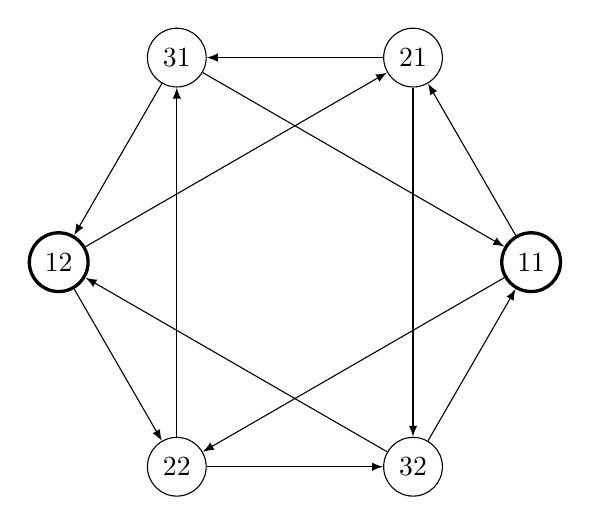
\begin{tikzpicture}
	\tikzstyle{every node}=[draw, shape=circle];

	\node[very thick] (x1) at (0:3) {$11$};
	\node (y1) at (60:3) {$21$};
	\node (z1) at (120:3) {$31$};
		
	\node[very thick] (x2) at (180:3) {$12$};
	\node (y2) at (240:3) {$22$};
	\node (z2) at (300:3) {$32$};

	\draw[-latex] (x1) -- (y1);
	\draw[-latex] (x1) -- (y2);

	\draw[-latex] (x2) -- (y1);
	\draw[-latex] (x2) -- (y2);

	\draw[-latex] (y1) -- (z1);
	\draw[-latex] (y1) -- (z2);

	\draw[-latex] (y2) -- (z1);
	\draw[-latex] (y2) -- (z2);

	\draw[-latex] (z1) -- (x1);
	\draw[-latex] (z1) -- (x2);

	\draw[-latex] (z2) -- (x1);
	\draw[-latex] (z2) -- (x2);
\end{tikzpicture}
\caption{The graph $2 \oplus C_3$ with guessing number $2$.}
\label{fig:2C3}
\end{figure}
\end{example}

A \BF{fractional cycle packing}\index{fractional cycle packing} of a graph $D$ is a family of cycles $B_1, \dots, B_s$ of $D$ together with non-negative weights $w_1, \dots, w_s$ such that
\[
	\sum_{i : v \in B_i} w_i \le 1 \quad \forall\, v \in [n].
\]
In particular, a cycle packing is a fractional cycle packing where the weights belong to $\{0,1\}$. The maximum value of $\sum_{i=1}^s w_i$ over all fractional cycle packings is the \BF{fractional packing number}\index{number!fractional packing} and is denoted by $\fractionalPacking(D)$. Since a cycle packing is a particular fractional cycle packing, we have $\fractionalPacking(D) \ge \packing(D)$.

Similarly, a \BF{fractional clique cover}\index{fractional clique cover} of a graph $D$ is a family of cliques $H_1, \dots, H_t$ of $D$ together with non-negative weights $w_1, \dots, w_t$ such that
\[
	\sum_{i : v \in H_i} w_i \ge 1 \quad \forall\, v \in [n].
\]
Again, a clique cover is a fractional clique cover where all the weights belong to $\{0,1\}$. The minimum value of $\sum_{i=1}^t w_i$ over all fractional clique covers is the \BF{fractional clique cover number}\index{number!fractional clique cover} and is denoted by $\fractionalCliqueCover(D)$. Since a clique cover is a particular fractional clique cover, we have $\fractionalCliqueCover(D) \le \cliqueCover(D)$.


Fractional graph theory is a wide topic, but it is beyond the scope of this book. The interested reader is directed to the book by Scheinerman and Ullman \cite{SU97}. We only need the following results. For any $D$, $\fractionalPacking(D)$ and $\fractionalCliqueCover(D)$ are rational numbers. More precisely, there exist $k, k'$ such that 
\[
	\packing(k \oplus D) = k \fractionalPacking(D), \quad \cliqueCover(k' \oplus D) = k' \fractionalCliqueCover(D).
\]
Combining with Theorem \ref{th:fractional}, we obtain the following lower bounds on the asymptotic guessing number.

\begin{corollary} \label{cor:fractional}
For any $D$, there exist $k$ and $k'$ such that for all $q \ge 2$,
\begin{align*}
	\guessing(D) \ge \guessing(D,q^k) &\ge \fractionalPacking(D),\\
	\guessing(D) \ge \guessing(D,q^{k'}) &\ge n - \fractionalCliqueCover(D).
\end{align*}
\end{corollary}













\subsection{Guessing number of special classes of graphs}



%\subsection{Graphs with small feedback vertex sets}

The feedback bound is always achieved when $\feedback(D) = 0$ (i.e., if $D$ is acyclic); we shall prove that it is also achieved for $\feedback(D) = 1$ (for the strict guessing number) and $\feedback(D) = 2$ (for the guessing number).


\begin{theorem} \label{cor:feedback=1}
If $\feedback(D) = 1$, then $\guessing[D,q] = 1$ for all $q \ge 2$.
\end{theorem}

\begin{proof}
This is an easy consequence of the feedback bound (Theorem~\ref{th:fixed_points_feedback}) and Proposition~\ref{pro:strict_packing_lower_bound}.
\end{proof}



The situation for feedback of size $2$ was settled by Shenvi and Dey \cite{SD10}.


\begin{theorem} \label{th:guessing_number_feedback2}
If $\feedback(D) = 2$, then $\guessing(D,q) = 2$ for all $q \ge 2$.
\end{theorem}

We delay the proof until Chapter \ref{ch:optimality_feedback}.


%\subsection{Graphs with a loop on every vertex} \label{sec:guessing_loops}

We now determine the strict guessing number of loop-full graphs, i.e. for transversal number $n$ (the case $\feedback(D) = n-1$ is settled in Exercise \ref{exerc:feedback=n-1}). For any loopless graph $D$, we denote the graph obtained from $D$ by adding a loop on each vertex by $\loopfull{D}$. Clearly, $\guessing(\loopfull{D}, q) = n$; moreover, $\guessing[\loopfull{D}, q] = n$ if and only if $D$ is empty (since $\loopfull{D}$ is then the interaction graph of the identity function).

For any loopless $D$, an \BF{in-dominating set}\index{set!in-dominating} is a set of vertices $X \subseteq [n]$ such that for all $v \in [n]$ with positive in-degree, either $v \in X$ or $\NIn(v) \cap X \ne \emptyset$. Denote the number of in-dominating sets of $D$ of size $k$ by $I_k(D)$.


\begin{theorem}[\cite{GRF16}] \label{th:g_strict_loops}
For any loopless graph $D$ and $q\geq 2$, 
\[
	\guessing[\loopfull{D}, q] = \log_q \sum_{k=0}^n (q-1)^k I_k(D).
\]
\end{theorem}

\begin{proof}
In the proof, the underlying graph considered is always $\loopfull{D}$ and not $D$. We define the function $g \in \functions[\loopfull{D},q]$ as
\[
	g_v(x) := \begin{cases}
	x_v & \mbox{if } \dIn(v) = 1\\
	x_v + \one{ x_{\NIn(v)} = (0,\dots,0) } & \mbox{otherwise}.
	\end{cases}
\]
For any $x$, $x = g(x)$ if and only if $\{v \in [n] : x_v \ne 0\}$ is an in-dominating set. This proves the lower bound.

Now let $f\in \functions[\loopfull{D},q]$ with guessing number $\guessing[\loopfull{D}, q]$. Any local function of $f$ is expressed as
\[
	f_v(x) = \begin{cases}
	a(x_v) & \mbox{if } \dIn(v) = 1\\
	x_v + h_v(x_{\NIn(v)}) & \mbox{otherwise},
	\end{cases}
\]
where $h_v(x_{\NIn(v)}) = f_v(x) - x_v \mod q$. It is clear that the optimal choice for the function $a$ is simply $a(x_v) = x_v$. Therefore, we only focus on the case where $\dIn(v) \ge 2$ henceforth.

We now show that we can always assume that $h_v$ takes a non-zero only once. Let $Y = \{y \in \(q\)^{\dIn(v)} : h_v(y) \ne 0\}$ and let $y^v \in Y$. Now, let $f'$ such that $f'_u = f_u$ for all $u \ne v$ and
\[
	f'_v(x) = x_v + \one{x_{\NIn(v)} = y^v}  \mod q.
\]
Suppose $f(x) = x$, then $f'_u(x) = f_u(x) = x_u$ for all $u \ne v$; moreover, $x_{\NIn(v)} \notin Y$ hence $x_{\NIn(v)} \ne y^v$ and $f'_v(x) = f_v(x) = x_v$. Therefore, $|\Fix(f')| \ge |\Fix(f)|$.

Hence we can consider $f'$ instead. We now show that choosing $y^v = (0,\dots,0)$ for any vertex $v$ maximises the number of fixed points. Consider a vertex $w$ and define a new function $f''$ as
\begin{align*}
	f''_u &= f'_u \quad \forall\, u \notin \NOut(w),\\
	f''_v(x) &= x_v + \one{x_{\NIn(v)} = z^v} \quad \forall\, v \in \NOut(w),
\end{align*}
where $z^v_u = y^v_u$ if $u \ne w$ and $z^v_w = 0$. 
Let $x' \in \Fix(f') \setminus \Fix(f'')$. Then there exists $v \in \NOut(w)$ such that $z^v = x'_{\NIn(v)} \ne y^v$. Defining $x''$ by only changing the $w$-coordinate of $x'$ to $x''_w := y^v_w$ we obtain $z^v \ne x''_{\NIn(v)} = y^v$ and $z^u \ne x''_{\NIn(u)}$ for all $u \in \NOut(w) \setminus v$ (because $x''_w > 0 = z^u_w$). Thus $x'' \in \Fix(f'') \setminus \Fix(f')$. Hence, there is an injection from $\Fix(f') \setminus \Fix(f'')$ to $\Fix(f'') \setminus \Fix(f')$, thus $f''$ has at least as many fixed points as $f'$.

Thus, we can always choose $z^v_w = 0$ for all $v$ and all $w$, which yields the function $g$. 
\end{proof}


\begin{corollary} \label{cor:g_strict_loops}
For any loopless graph $D$ and $q\ge 2$, we have 
\[
	\guessing[\loopfull{D}, q] \ge n \log_q (q-1) + \log_q \left(1 + \frac{n}{q-1} \right).
\]
\end{corollary}

\begin{proof}
For any vertex $v \in [n]$, $-v$ is an in-dominating set, hence $I_{n-1}(D) = n$. Also, since $[n]$ is an in-dominating set, $I_n(D) = 1$. Therefore, $\guessing[\loopfull{D}, q] \ge \log_q \left( n(q-1)^{n-1} + (q-1)^n \right)$.
\end{proof}

\begin{example} \label{ex:g_strict_loops}
In general, computing the sum $\sum_k (q-1)^k I_k(D)$ is \#P-Complete. However, we can exhibit several special cases for which the formula is easy to derive. We assume $n \ge 2$.
\begin{itemize}
	\item For the clique $K_n$, we have $I_0(K_n) = 0$ and $I_k(K_n) = \binom{n}{k}$ for all $1 \le k \le n$. Therefore, $\sum_k (q-1)^k I_k(K_n) = q^n - 1$ and
	\[
		\guessing[\loopfull{K_n}, q] = \log_q( q^n - 1 ).
	\]
	
	\item For the transitive tournament $T_n$ (with arcs $uv$ for all $u < v$), a set of vertices is an in-dominating set if and only if it contains either the first or the second vertex. Thus $I_k(T_n) = \binom{n}{k} - \binom{n-2}{k}$ and $\sum_k (q-1)^k I_k(T_n) = q^n - q^{n-2}$, hence
	\[
		\guessing[\loopfull{T_n}, q] = n-2 + \log_q(q^2-1).
	\]
		
	\item For the undirected star $S_n$ (with arcs $vn$ and $nv$ for all $1 \le v \le n-1$), $I_{n-1}(S_n) = n$ and $I_k(S_n) = \binom{n-1}{k-1}$ otherwise. Thus
	\[
		\guessing[\loopfull{S_n}, q] = \log_q( q^n - q^{n-1} + (q-1)^{n-1} ).
	\]
\end{itemize}
\end{example}












\section{Guessing graph} \label{sec:guessing_graph}

In this section, we introduce a simple graph on all possible states of a graph, called guessing graph, where an independent set corresponds to a set of fixed states of a function. As a result, the guessing number of the graph is equivalent to the logarithm of the independence number of the associated graph. The guessing graph approach then converts the problem of finding a function with maximum number of fixed points into a purely graph theoretical problem. The guessing graph was first proposed in \cite{BBJK06} under the name ``confusion graph'' and then independently in \cite{GR11}. Most results in this section come from \cite{GR11}.



\subsection{Guessing graph and guessing number} \label{sec:guessing_graph_definition}


For any graph $D$ and any $q \ge 2$, the \BF{$q$-guessing graph}\index{graph:guessing} of $D$, denoted by $\guessingGraph(D,q)$, is the simple graph on $\(q\)^n$ where two states $x, y \in \(q\)^n$ are adjacent if and only if there is no $f \in \functions(D,q)$ such that $x, y \in \Fix(f)$.

Proposition \ref{prop:properties_guessing_graph} below enumerates some properties of the guessing graph. In particular, Property \ref{it:E} provides a concrete and elementary description of the edge set which makes adjacency between two states easily decidable.

\begin{proposition} \label{prop:properties_guessing_graph}
The $q$-guessing graph $\guessingGraph(D,q)$ of a graph $D$ on $n$ vertices satisfies the following properties:
\begin{enumerate}
    \item \label{it:E} Its edge set is 
	\begin{align*}
		E &= \bigcup_{v=1}^n E_v,\\
		E_v &:= \{xy : x_{\NIn(v)} = y_{\NIn(v)}, x_v \ne y_v\}.
	\end{align*}
	
	\item \label{it:d(D,q)} It is regular with degree
	\[
		d(\guessingGraph(D,q)) = \sum_{I \mathrm{independent}} (-1)^{|I|-1} (q-1)^{|I|} q^{n - |\NIn(I)| - |I|}.
	\]
%	where $\NIn(I)$ is the union of all the in-neighborhoods of vertices in $I$.
	
	\item \label{it:vertex_transitive} It is vertex-transitive. More precisely, $\Aut(\guessingGraph(D,q)) \ge \Aut(H(n,q))$. 
\end{enumerate}
\end{proposition}

\begin{proof}
We first prove Property \ref{it:E}. Let $xy \in E_v$ for some $v$ and let $f \in \functions(D,q)$ with $x \in \Fix(f)$. Then 
\[
	f_v(y_{\NIn(v)}) = f_v(x_{\NIn(v)}) = x_v \ne y_v,
\]
hence $y\not\in\Fix(f)$. Conversely, if $xy \notin E$ then any $f \in \functions(D,q)$ satisfying $f_v (x_{\NIn(v)}) = x_v$ and $f_v(y_{\NIn(v)}) = y_v$ for all $v$ fixes both $x$ and $y$.

Property \ref{it:vertex_transitive} follows this observation: $xy \in E$ if and only if $(x-y)_{\NIn(v)} = 0$ and $(x-y)_v \ne 0$ for some $v$. Since the guessing graph is vertex-transitive it is regular and hence we determine the degree of the all-zero state $0$. For any $R \subseteq [n]$, denote $E_R := \bigcap_{v \in R} E_v$ and the set of edges in $E_R$ containing $0$ as $E_R(0)$. By the inclusion-exclusion principle, we have
\[
	\degree(\guessingGraph(D,q)) = \degree(0) = \left|\bigcup_{i=1}^n E_v(0) \right| = \sum_{R \subseteq [n]} (-1)^{|R|-1} |E_R(0)|.
\]
Hence we only have to determine $|E_R(0)|$ for all $R \subseteq [n]$. The states $y$ adjacent to $0$ satisfy $y_R>0$ and $y_{\NIn(R)} = 0$, while $y_{V \setminus( \NIn(R) \cup R)}$ is arbitrary. If $R$ is not independent, $R \cap \NIn(R) \ne \emptyset$ and the two conditions are contradictory, thus $|E_R(0)| = 0$; otherwise $R \cap \NIn(R) = \emptyset$ and there are $(q-1)^{|R|} q^{n - |\NIn(R)| - |R|}$ choices for $y$. 
\end{proof}

The guessing graph of some particular graphs can be characterized.

\begin{example} \label{ex:guessing_graph}
The following guessing graphs are easy to determine.
\begin{itemize}
	\item If $D$ is acyclic, let us sort the vertices in topological order. Consider two distinct states $x,y \in \(q\)^n$ and let $l = \min\{v : x_v \ne y_v \}$, then $x_{\NIn(l)} = y_{\NIn(l)}$ and $xy \in E_l$. Thus the $q$-guessing graph of an acyclic graph is the clique $K_{q^n}$.


	\item For the clique $K_n$, we have $E_v = \{xy: x_{- v} = y_{- v}, x_v \ne y_v \}$ and hence $x$ and $y$ are adjacent if and only if they differ in exactly one coordinate. The $q$-guessing graph of the clique $K_n$ is the Hamming graph $H(n,q)$.
	
	\item We now consider the cycle $\vec{C}_n$. Suppose $x$ and $y$ are distinct and non-adjacent, then there exists $v$ such that $x_v \ne y_v$. Since $xy \notin E_v$, we have $x_{v-1} \ne y_{v-1}$ (where $v-1$ is the in-neighbour of $v$ in $\vec{C}_n$). Applying this recursively, we obtain that all coordinates of $x$ and $y$ must be distinct. Conversely, if $x_v \ne y_v$ for all $v$, then it is clear that $x$ and $y$ are not adjacent. Therefore,
 $E(\guessingGraph(\vec{C}_n, q)) = \{xy: \dH(x,y) \le  n-1\}$.
	
	\item It is easy to check that the $q$-guessing graph of a loop-full graph is empty.
\end{itemize}
\end{example}


Clearly, the set of fixed points of any function in $\functions(D,q)$ is an independent set of the guessing graph $\guessingGraph(D,q)$. Theorem \ref{th:fixed_is_independent} below asserts the converse: any independent set of $\guessingGraph(D,q)$ can be fixed by some function in $\functions(D,q)$.

\begin{theorem} \label{th:fixed_is_independent}
For any $f \in \functions(D,q)$, $\Fix(f)$ is an independent set in $\guessingGraph(D,q)$. Conversely, for any independent set $Z$ of $\guessingGraph(D,q)$, there exists $f \in \functions(D,q)$ such that $Z \subseteq \Fix(f)$. Thus
\begin{equation} \nonumber
	\guessing(D,q) = \log_q \independence(\guessingGraph(D,q)).
\end{equation}
\end{theorem}

\begin{proof}
By definition, any set of fixed points of some function form an independent set in the guessing graph. Conversely, let $Z = \{z^1, \dots, z^k\}$ be an independent set of the guessing graph. Then define $f$ by
\[
f_v(x)=
\begin{cases}
z^i_v&\text{ if $x_{\NIn(v)} = z^i_{\NIn(v)}$ for some $1\le i\le k$}\\
0&\text{ otherwise.}
\end{cases}
\]
This is a non-ambiguous assignment, as either $z^i_{\NIn(v)} \ne z^j_{\NIn(v)}$ (and the assignments are independent) or $z^i_{\NIn(v)} = z^j_{\NIn(v)}$ and $z^i_v = z^j_v$ (the same assignment) for all $i,j \in \{1, \dots,k\}$. Then $f \in \functions(D,q)$ and $Z\subseteq \Fix(f)$. 
\end{proof}

The guessing numbers of the graphs mentioned in Example \ref{ex:guessing_graph} were already determined in Section \ref{sec:guessing_number}. However, the proof becomes straightforward using Theorem \ref{th:fixed_is_independent}.

\begin{example} \label{ex:g_from_guessing_graph}
The following statements hold for all $q$. If $D$ is acyclic, then $\guessing(D,q) = 0$. Also, the clique satisfies $\guessing(K_n, q) = n-1$. Finally, for the cycle we have $\guessing(\vec{C}_n, q) = 1$.
\end{example}

The clique $K_3$ and its binary guessing graph, given by the cube $H(3,2)$, are illustrated in Figure \ref{fig:guessing_butterfly}. Throughout this section, we shall highlight a maximum independent set of the guessing graph in bold with thick contours.

\begin{figure}
\centering
	\subfloat[$K_3$]
	{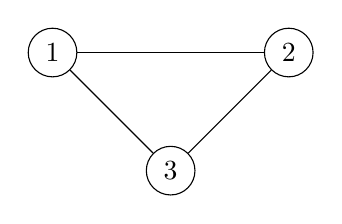
\begin{tikzpicture}
	\tikzstyle{every node}=[draw,shape=circle];
	
	\node (x) at (0,3) {$1$};
	\node (y) at (3,3) {$2$};
	\node (z) at (1.5,1.5) {$3$};
	
	\draw (x) -- (y);
	\draw (x) -- (z);
	\draw (y) -- (z);
	\end{tikzpicture}
	} \hspace{1cm}
\subfloat[A maximum independent set in the guessing graph $\guessingGraph(K_3,2) = H(2,3)$]{
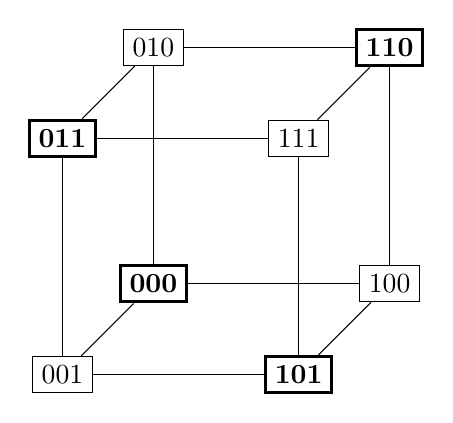
\begin{tikzpicture}
	\tikzstyle{every node}=[draw];

	\node[very thick] (000) at (0,0,0) {${\bf 000}$};
	\node (001) at (0,0,3) {001};
	\node (010) at (0,3,0) {010};
	\node[very thick] (011) at (0,3,3) {${\bf 011}$};
	\node (100) at (3,0,0) {100};
	\node[very thick] (101) at (3,0,3) {${\bf 101}$};
	\node[very thick] (110) at (3,3,0) {${\bf 110}$};
	\node (111) at (3,3,3) {111};
	
	\draw (000) -- (001);
	\draw (000) -- (010);
	\draw (000) -- (100);
	\draw (001) -- (011);
	\draw (001) -- (101);
	\draw (010) -- (011);
	\draw (010) -- (110);
	\draw (100) -- (101);
	\draw (100) -- (110);
	\draw (101) -- (111);
	\draw (110) -- (111);
	\draw (011) -- (111);
\end{tikzpicture}}
\caption{The guessing graph $\guessingGraph(K_3,2)$.}
\label{fig:guessing_butterfly}
\end{figure}






\subsection{Results based on the guessing graph} \label{sec:bound_guessing_graph}


We now investigate the properties of the guessing graph and thus derive bounds on the guessing number of graphs. 

The following proposition gives a lower bound on the guessing number based on the degree of the guessing graph, which shall be refined for large alphabets in Proposition \ref{prop:bound_code}.

\begin{proposition} \label{prop:lower_g_d}
For any non-acyclic graph $D$ and any $q$,
\begin{align*} 
	\guessing(D,q) &\ge n+\log_q \frac{3}{2} + \log_q \left\{1 - \sqrt{1 - \frac{4}{3 (d(\guessingGraph(D,q)) + 1)}} \right\}\\
	&\ge \dInMin(D) - \log_q n.
\end{align*}
\end{proposition}

\begin{proof}
For a non-complete $\kappa$-connected graph $G$ on $m$ vertices which is regular with degree $d$, the independence number is lower bounded by \cite{HS01}
\begin{equation} \label{eq:lower_alpha}
	\alpha(G) \geq \frac{m(d+1)}{\kappa} \left\{ 1 - \sqrt{1 - 2\frac{\kappa}{(d+1)^2}} \right\} \geq \frac{m}{d+1}.
\end{equation}
Since the guessing graph is vertex-transitive, its connectivity is at least $\frac{2 (d+1)}{3}$ by \cite{Bab94}. By applying the first inequality in (\ref{eq:lower_alpha}) and Theorem~\ref{th:fixed_is_independent}, we easily obtain the first lower bound above. Call this term $L$; the second inequality in (\ref{eq:lower_alpha}) yields $L \ge n - \log_q(d(\guessingGraph(D,q)) + 1)$. We have $d(\guessingGraph(D,q)) = |\bigcup_v E_v (0)|$, where $|E_v (0)| = (q-1)q^{n - \dIn(v) - 1}$ as seen in the proof of Proposition \ref{prop:properties_guessing_graph}, hence $d(\guessingGraph(D,q)) \le nq^{n-\dInMin(D)} - 1$. The second lower bound then follows.
\end{proof}

\begin{corollary} \label{cor:guessing>dinmin}
For any $D$, $\guessing(D) \ge \dInMin(D)$.
\end{corollary}



If $H$ is a spanning subgraph of $D$, then it is easy to verify that $\guessingGraph(H,q) \supseteq \guessingGraph(D,q)$, hence $\guessing(H, q) \le \guessing(D,q)$. On the other hand, the guessing graph of any induced subgraph can be viewed as a subgraph of the guessing graph of $D$. For any induced subgraph $H$ of $D$ and any $e \in \(q\)^{n-|H|}$, we denote the subgraph of $\guessingGraph(D,q)$ induced by all states satisfying $x_{- H} = e$ by $\guessingGraph(D,q)_H + e$. 

\begin{lemma} \label{lemma:guessing_subgraph}
For any induced subgraph $H$ of $D$ and any $e \in \(q\)^{n-|H|}$, we have $\guessingGraph(D,q)_H +e \cong \guessingGraph(H,q)$.
\end{lemma}


\begin{proof}
Two states $x,y$ are adjacent in $\guessingGraph(D,q)_H + e$ if and only if there exists $v\in V(H)$ such that $x_v \ne y_v$, $x_{\NIn(v)} = y_{\NIn(v)}$. Since $x_{- H} = y_{- H} = e$, this is equivalent to $x_v \ne y_v$, $x_{\NIn(v) \cap H} = y_{\NIn(v) \cap H}$, hence $x_H$ and $y_H$ are adjacent in $\guessingGraph(H,q)$.
\end{proof}

\begin{corollary} \label{cor:lower_omega}
We have $\log_q \clique(\guessingGraph(D,q)) \ge n - \feedback(D)$.
\end{corollary}

\begin{proof}
Let $H$ be a maximum induced acyclic subgraph of $D$, then $\guessingGraph(D,q)_H + e \cong \guessingGraph(H,q)$, which by Example \ref{ex:guessing_graph} is a clique on $q^{|H|}$ vertices.
\end{proof}


The proof of Corollary \ref{cor:lower_omega} actually indicates that the family $\{\guessingGraph(D,q)_H + e\}$ for all $e \in \(q\)^{\feedback(D)}$ forms a partition of the vertex set of $\guessingGraph(D,q)$ into cliques of size $q^{n - \feedback(D)}$.

Proposition \ref{prop:summary_bounds} below combines the results derived above with further graph-theoretic results.

\begin{proposition} \label{prop:summary_bounds}
For any non-acyclic graph $D$ and any $q \ge 2$,
%\begin{align*}
%	&\dInMin(D) - \log_q n \le n - \log_q d(\guessingGraph(D,q))\\
%	&\le n - \log_q \chromatic(\guessingGraph(D,q))\\
%	&\le \guessing(D,q) = \log_q \alpha(\guessingGraph(D,q))\\
%	&\le n - \log_q \clique(\guessingGraph(D,q))\\
%	&\le \feedback(D).
%\end{align*}
\begin{alignat*}{3}
	\guessing(D,q) &= \log_q \alpha(\guessingGraph(D,q)) &&\le n - \log_q \clique(\guessingGraph(D,q)) && \le \feedback(D),\\
	\guessing(D,q) &\ge  n - \log_q \chromatic(\guessingGraph(D,q)) &&\ge  n - \log_q d(\guessingGraph(D,q)) && \ge \dInMin(D) - \log_q n.
\end{alignat*}
\end{proposition}

\begin{proof}
We have already justified the first inequality in the proof of Proposition \ref{prop:lower_g_d}, the equality in Theorem \ref{th:fixed_is_independent} and the last inequality in Corollary \ref{cor:lower_omega}.

The remaining inequalities come from the following graph-theoretic results. For a connected vertex-transitive simple graph $H$ which is neither an odd cycle nor a complete graph, we have \cite[Corollary 7.5.2]{GR01}
\begin{equation} \label{eq:parameters_graph} \nonumber
	\clique(H) \le  \frac{|V(H)|}{\independence(H)} \le \chromatic(H) \le d(H).
\end{equation}
\end{proof}


A code with minimum Hamming distance $d$ can be viewed as an independent set of the graph where two states are adjacent if and only if they differ by at most $d-1$ coordinates. Therefore, finding a maximum code with a prescribed minimum distance can be viewed as finding the maximum independent set of this graph. On the other hand, as seen in Proposition \ref{prop:properties_guessing_graph}, whether two states are adjacent in the guessing graph is completely determined by the coordinates in which they differ. Therefore, determining the guessing number of a graph is a similar problem to that of finding error-correcting codes with maximum cardinality. In particular, Example \ref{ex:guessing_graph} indicates that the guessing number of the clique $K_n$ (the cycle $\vec{C}_n$, respectively) is equivalent to the maximum cardinality of a code of length $n$ with minimum distance $2$ (minimum distance $n$, respectively). In Proposition \ref{prop:bound_code}, we generalise this idea and show that a code with large enough minimum distance is a set of fixed points of some function in $\functions(D,q)$.



\begin{proposition}[The code lower bound] \label{prop:bound_code}
For any $D$ and any $q$,
\[
	\guessing(D,q) \ge \log_q \AH(n, q, n-\dInMin(D) + 1).
\]
In particular, $\guessing(D,q) \ge \dInMin(D)$ if there exists a $q$-ary MDS code of length $n$ and minimum distance $\dInMin(D)$.
\end{proposition}

\begin{proof}
First, for any two states $x,y \in \(q\)^n$ adjacent in the guessing graph of $D$, we have $(x-y)_{\NIn(v)} = 0$ for some $v$, hence $\dH(x,y) \le n - \dIn(v) \le n- \dInMin(D)$. Therefore, in any code with minimum distance $n-\dInMin(D) + 1$, the codewords are not adjacent in the guessing graph, hence they form a set of fixed states. In particular, using an MDS code yields the lower bound $\guessing(D,q) \ge \dInMin(D)$ for the mentioned parameter values.
\end{proof}






\subsection{Guessing graph of graph unions} \label{sec:guessing_graph_graph_union}

We now investigate how the guessing graph behaves when we consider the (disjoint, unidirectional and bidirectional) union of two graphs $D_1$ and $D_2$ with disjoint vertex sets. As we shall see, they will correspond to different products of graphs, and provide elegant proofs of the results of Section \ref{sec:guessing_union}. We shall illustrate these unions by the following example: $D_1 = K_2$ and $D_2 = \vec{P}_2$ illustrated in Figure \ref{fig:P1_K2}.

\begin{figure}
\centering
\subfloat[$K_2$]{
	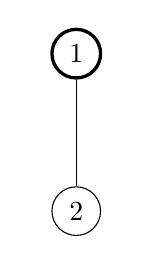
\begin{tikzpicture}
		\node (a) at (-0.5,0) {};
		\node (b) at (0.5,0) {};
		
		\node[draw, shape=circle, very thick] (0) at (0,2) {$1$};
		\node[draw, shape=circle] (1) at (0,0) {$2$};
		
		\draw (0) -- (1);
	\end{tikzpicture}}\hspace{1cm}
\subfloat[$\guessingGraph(K_2,2) = H(2,2)$]{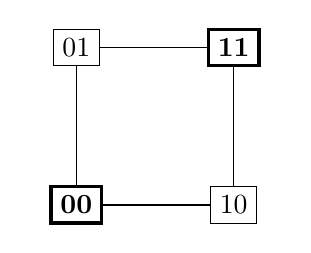
\begin{tikzpicture}
	\node (a) at (-0.5,0) {};
	\node (b) at (2.5,0) {};
	
	\tikzstyle{every node}=[draw];
		\node[very thick] (00) at (0,0) {${\bf 00}$};
		\node (01) at (0,2) {01};
		\node (10) at (2,0) {10};
		\node[very thick] (11) at (2,2) {${\bf 11}$};
		
		\draw (00) -- (01);
		\draw (00) -- (10);
		\draw (11) -- (01);
		\draw (11) -- (10);
	\end{tikzpicture}} \hspace{1cm}
\subfloat[$\vec{P}_2$]{
	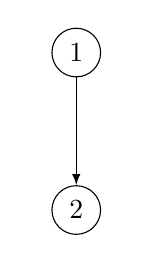
\begin{tikzpicture}
		\node (a) at (-0.5,0) {};
		\node (b) at (0.5,0) {};

		\node[draw, shape=circle] (0) at (0,2) {$1$};
		\node[draw, shape=circle] (1) at (0,0) {$2$};
		
		\draw[-latex] (0) -- (1);
	\end{tikzpicture}} \hspace{1cm}
\subfloat[$\guessingGraph(\vec{P}_2,2) = K_4$]{
	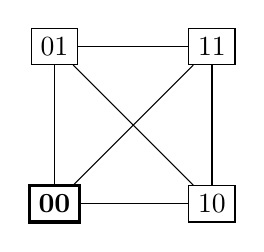
\begin{tikzpicture}
	\tikzstyle{every node}=[draw];
		\node[very thick] (00) at (0,0) {${\bf 00}$};
		\node (01) at (0,2) {01};
		\node (10) at (2,0) {10};
		\node (11) at (2,2) {11};
		
		\draw (00) -- (01);
		\draw (00) -- (10);
		\draw (11) -- (01);
		\draw (11) -- (10);
		\draw (00) -- (11);
		\draw (10) -- (01);
	\end{tikzpicture}}
\caption{The graphs $K_2$ and $\vec{P}_2$ and their guessing graphs.}
\label{fig:P1_K2}
\end{figure}


We now review three products of undirected graphs. All products of two graphs $D_1$ and $D_2$ have $V(D_1) \times V(D_2)$ as vertex set; note that $V(D_1)$ and $V(D_2)$ are not necessarily disjoint. We denote $n_1 := |V(D_1)|$ and $n_2 := |V(D_2)|$, and we further denote two adjacent vertices $u$ and $v$ in a simple graph by $u \sim v$.
\begin{itemize}
	\item First, in the \BF{co-normal product}\index{graph product!co-normal} $D_1 \oplus D_2$, we have $(u_1,u_2) \sim (v_1,v_2)$ if and only if $u_1 \sim v_1$ or $u_2 \sim v_2$. We have
	\begin{equation} \label{eq:alpha_conormal}
		\independence(D_1 \oplus D_2) = \independence(D_1) \independence(D_2).
	\end{equation}
		
	\item Second, in the \BF{lexicographic product}\index{graph product!lexicographic} (also called composition) $D_1 \cdot D_2$, we have $(u_1,u_2) \sim (v_1,v_2)$ if and only if either $u_1 = v_1$ and $u_2 \sim v_2$, or $u_1 \sim v_1$. Although this product is not commutative, we have
	\begin{equation} \label{eq:alpha_lexicographic} \nonumber
		\independence(D_1 \cdot D_2) = \independence(D_1) \independence(D_2).
	\end{equation}
	
	\item Third, in the \BF{cartesian product} \label{graph product!cartesian} $D_1 \, \Box \, D_2$, we have $(u_1,u_2) \sim (v_1,v_2)$ if and only if either $u_1 = v_1$ and $u_2 \sim v_2$, or $u_2 = v_2$ and $u_1 \sim v_1$. We have
\[	
	\independence(D_1 \, \Box \, D_2) \le \min\{ n_1 \independence(D_2), n_2 \independence(D_1) \}.
\]
\end{itemize}
Exercise \ref{exerc:graph_products} asks for the proofs of these properties.


\begin{proposition} \label{prop:disjoint_conormal}
For all graphs $D_1$, $D_2$ with disjoint vertex sets and any $q \ge 2$,
\begin{equation} \label{eq:disjoint_conormal} %\nonumber
	\guessingGraph(D_1 \cup D_2,q) \cong \guessingGraph(D_1,q) \oplus \guessingGraph(D_2,q).
\end{equation}
Hence $\guessing(D_1 \cup D_2, q) = \guessing(D_1, q) + \guessing(D_2, q)$.
\end{proposition}

\begin{proof}
Let $x, y \in \(q\)^n$ (where $n = |V(D_1)| + |V(D_2)|$) and $x_{D_1} = x^1$, $y_{D_1} = y^1$ and similarly for $D_2$. They are adjacent in $\guessingGraph(D_1 \cup D_2,q)$ if and only if there exists $v$ in $D_1$ or in $D_2$ such that $x_v \ne y_v$ and $x_{\NIn(v)} = y_{\NIn(v)}$. Since the neighbourhood of $v$ entirely lies in $D_1$ if $v \in D_1$ (and similarly for $D_2$), this is equivalent to $x^1_v \ne y^1_v$, $x^1_{\NIn(v)} = y^1_{\NIn(v)}$ or $x^2_v \ne y^2_v$, $x^2_{\NIn(v)} = y^2_{\NIn(v)}$. Therefore, this is equivalent to $x^1 \sim y^1$ in $\guessingGraph(D_1,q)$ or $x^2 \sim y^2$ in $\guessingGraph(D_2,q)$, which yields (\ref{eq:disjoint_conormal}). Finally, (\ref{eq:alpha_conormal}) gives the guessing number of the disjoint union.
\end{proof}

\begin{example} \label{ex:disjoint_union}
The guessing graph of the disjoint union of $K_2$ and $\vec{P}_2$ is illustrated in Figure \ref{fig:disjoint_ex} (we represent the states in hexadecimal form). Because it is a very dense graph, we only show which states are adjacent to the all-zero state. It is clear that $\independence(\guessingGraph(K_2 \cup \vec{P}_2),2) = 2$ and hence $\guessing(K_2 \cup \vec{P}_2, 2) =1$.

\begin{figure}
\centering
\subfloat[$K_2 \cup \vec{P}_2$]{
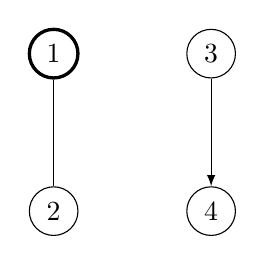
\begin{tikzpicture}
	\tikzstyle{every node}=[draw, shape=circle];
	
	\node[very thick] (a) at (0,2) {$1$};
	\node (b) at (0,0) {$2$};
	\node (c) at (2,2) {$3$};
	\node (d) at (2,0) {$4$};

	\draw (a) -- (b);
	\draw[-latex] (c) -- (d);
\end{tikzpicture}} \hspace{1cm}
\subfloat[$\guessingGraph(K_2 \cup \vec{P}_2,2) = H(2,2) \oplus K_4$]{
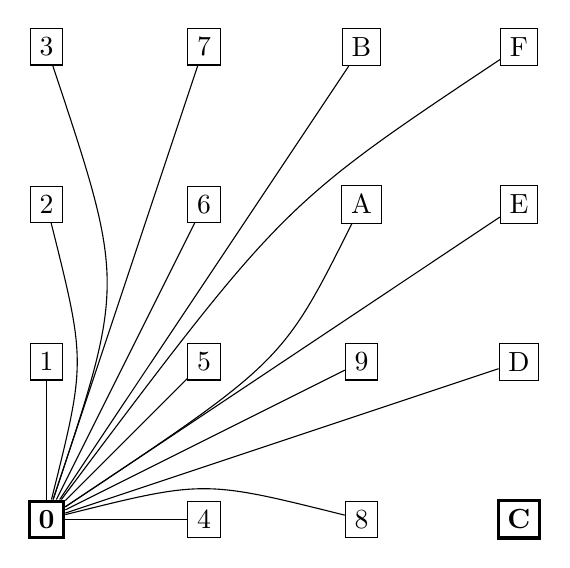
\begin{tikzpicture}
	\tikzstyle{every node}=[draw];

	\node[very thick] (0) at (0,0) {${\bf 0}$};
	\node (1) at (0,2) {1};
	\node (2) at (0,4) {2};
	\node (3) at (0,6) {3};
	\node (4) at (2,0) {4};
	\node (5) at (2,2) {5};
	\node (6) at (2,4) {6};
	\node (7) at (2,6) {7};
	\node (8) at (4,0) {8};
	\node (9) at (4,2) {9};
	\node (A) at (4,4) {A};
	\node (B) at (4,6) {B};
	\node[very thick] (C) at (6,0) {${\bf C}$};
	\node (D) at (6,2) {D};
	\node (E) at (6,4) {E};
	\node (F) at (6,6) {F};
		
	\draw (0) -- (1);
	\draw (0) -- (4);
	\draw (0) -- (7);
	\draw (0) -- (5);
	\draw (0) -- (6);
	\draw (0) -- (D);
	\draw (0) -- (9);
	\draw (0) -- (B);
	\draw (0) -- (E);

	\draw (0) .. controls(0.5,2) .. (2);
	\draw (0) .. controls(2,0.5) .. (8);
	\draw (0) .. controls(1,3) .. (3);
	\draw (0) .. controls(3,2) .. (A);
	\draw (0) .. controls(3,4) .. (F);
\end{tikzpicture}}
\caption{The disjoint union of $K_2$ and $\vec{P}_2$ and its guessing graph.}
\label{fig:disjoint_ex}
\end{figure}
\end{example}



\begin{proposition} \label{prop:unidirectional_lexicographic}
For all $D_1$, $D_2$ with disjoint vertex sets and any $q \ge 2$,
\begin{equation}\label{eq:unidirectional_lexicographic} \nonumber
	\guessingGraph(D_1 \vcup D_2,q) \cong \guessingGraph(D_1,q) \cdot \guessingGraph(D_2,q).
\end{equation}
Hence $\guessing(D_1 \vcup D_2, q) = \guessing(D_1, q) + \guessing(D_2, q)$.
\end{proposition}

The proof is similar to that of Proposition \ref{prop:disjoint_conormal}, hence it is omitted.


\begin{example} \label{ex:unidirectional_union}
The guessing graph of the unidirectional union of $K_2$ and $\vec{P}_2$ is illustrated in Figure \ref{fig:unidirectional_ex} below. Because it is a very dense graph, we only show which states are adjacent to the all-zero state. Although it is distinct to the guessing graph of the disjoint union, they both have the same independence number.
\end{example}

\begin{figure}
\centering
\subfloat[$K_2 \vcup \vec{P}_2$]{
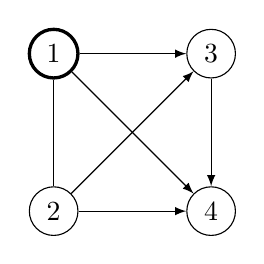
\begin{tikzpicture}
	\tikzstyle{every node}=[draw, shape=circle];
	
	\node[very thick] (a) at (0,2) {$1$};
	\node (b) at (0,0) {$2$};
	\node (c) at (2,2) {$3$};
	\node (d) at (2,0) {$4$};

	\draw (a) -- (b);
	\draw[-latex] (c) -- (d);
	\draw[-latex] (a) -- (c);
	\draw[-latex] (a) -- (d);
	\draw[-latex] (b) -- (c);
	\draw[-latex] (b) -- (d);
\end{tikzpicture}} \hspace{1cm}
\subfloat[$\guessingGraph(K_2 \vcup \vec{P}_2,2) = H(2,2) \cdot K_4$]{
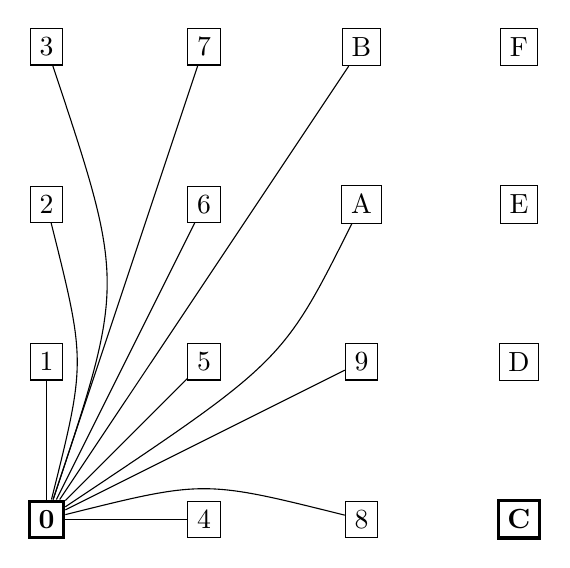
\begin{tikzpicture}
\tikzstyle{every node}=[draw];

	\node[very thick] (0) at (0,0) {${\bf 0}$};
	\node (1) at (0,2) {1};
	\node (2) at (0,4) {2};
	\node (3) at (0,6) {3};
	\node (4) at (2,0) {4};
	\node (5) at (2,2) {5};
	\node (6) at (2,4) {6};
	\node (7) at (2,6) {7};
	\node (8) at (4,0) {8};
	\node (9) at (4,2) {9};
	\node (A) at (4,4) {A};
	\node (B) at (4,6) {B};
	\node[very thick] (C) at (6,0) {${\bf C}$};
	\node (D) at (6,2) {D};
	\node (E) at (6,4) {E};
	\node (F) at (6,6) {F};
		
	\draw (0) -- (1);
	\draw (0) -- (4);
	\draw (0) -- (7);
	\draw (0) -- (5);
	\draw (0) -- (6);
	\draw (0) -- (9);
	\draw (0) -- (B);

	\draw (0) .. controls(0.5,2) .. (2);
	\draw (0) .. controls(2,0.5) .. (8);
	\draw (0) .. controls(1,3) .. (3);
	\draw (0) .. controls(3,2) .. (A);
\end{tikzpicture}}
\caption{The unidirectional union of $K_2$ and $\vec{P}_2$ and its guessing graph.}
\label{fig:unidirectional_ex}
\end{figure}


\begin{proposition} \label{prop:bidirectional_cartesian}
For any $D_1$, $D_2$ with disjoint vertex sets and any $q \ge 2$,
\[
	\guessingGraph(D_1 \bcup D_2,q) \cong \guessingGraph(D_1,q) \, \Box \, \guessingGraph(D_2,q).
\]
Hence, $\guessing(D_1 \bcup D_2, q) \le \min\{\guessing(D_1, q) + n_2, \guessing(D_2, q) + n_1 \}.$
\end{proposition}

Again, the proof is similar to that of Proposition \ref{prop:disjoint_conormal} and hence omitted. 


\begin{example}
The guessing graph of the bidirectional union of $K_2$ and $\vec{P}_2$ is depicted in Figure \ref{fig:bidirectional_ex}. In this case, we have $\guessing(K_2 \bcup \vec{P}_2, 2) = \guessing(\vec{P}_2, 2) + 2$. 

\begin{figure}
\centering
\subfloat[$K_2 \bcup \vec{P}_2$]{
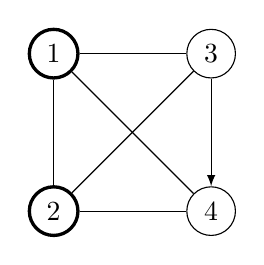
\begin{tikzpicture}
	\tikzstyle{every node}=[draw, shape=circle];
	
	\node[very thick] (a) at (0,2) {$1$};
	\node[very thick] (b) at (0,0) {$2$};
	\node (c) at (2,2) {$3$};
	\node (d) at (2,0) {$4$};

	\draw (a) -- (b);
	\draw[-latex] (c) -- (d);
	\draw (a) -- (c);
	\draw (a) -- (d);
	\draw (b) -- (c);
	\draw (b) -- (d);
\end{tikzpicture}} \hspace{1cm}
\subfloat[$\guessingGraph(K_2 \bcup \vec{P}_2,2) = H(2,2) \, \Box \, K_4$]{
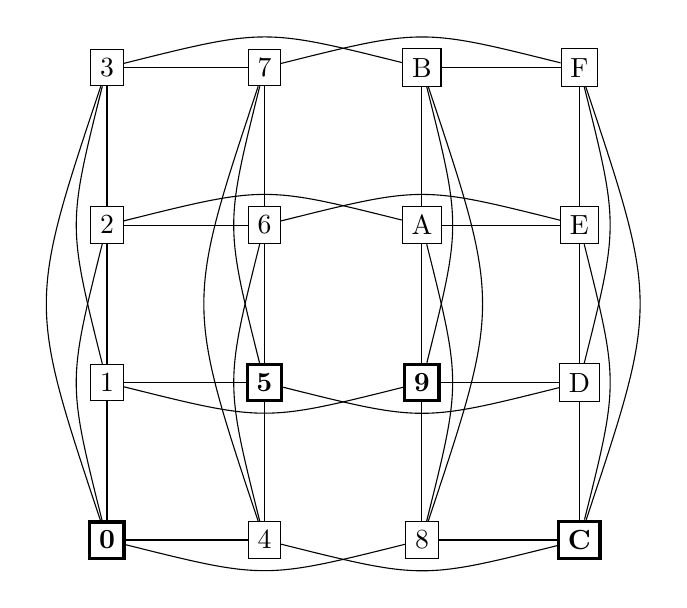
\begin{tikzpicture}
\tikzstyle{every node}=[draw];

	\node[very thick] (0) at (0,0) {${\bf 0}$};
	\node (1) at (0,2) {1};
	\node (2) at (0,4) {2};
	\node (3) at (0,6) {3};
	\node (4) at (2,0) {4};
	\node[very thick] (5) at (2,2) {${\bf 5}$};
	\node (6) at (2,4) {6};
	\node (7) at (2,6) {7};
	\node (8) at (4,0) {8};
	\node[very thick] (9) at (4,2) {${\bf 9}$};
	\node (A) at (4,4) {A};
	\node (B) at (4,6) {B};
	\node[very thick] (C) at (6,0) {${\bf C}$};
	\node (D) at (6,2) {D};
	\node (E) at (6,4) {E};
	\node (F) at (6,6) {F};
		
	\draw (0) -- (1);
	\draw (0) -- (4);
	\draw (0) .. controls(-0.5,2) .. (2);
	\draw (0) .. controls(2,-0.5) .. (8);
	\draw (0) .. controls(-1,3) .. (3);

	\draw (1) -- (2);
	\draw (1) -- (5);
	\draw (1) .. controls(-0.5,4) .. (3);
	\draw (1) .. controls(2,1.5) .. (9);

	\draw (2) -- (3);
	\draw (2) -- (6);
	\draw (2) .. controls(2,4.5) .. (A);

	\draw (3) -- (7);
	\draw (3) .. controls(2,6.5) .. (B);


	\draw (4) -- (5);
	\draw (4) .. controls(1,3) .. (7);
	\draw (4) .. controls(1.5,2) .. (6);
	\draw (4) .. controls(4,-0.5) .. (C);

	\draw (5) -- (6);
	\draw (5) .. controls(4,1.5) .. (D);
	\draw (5) .. controls(1.5,4) .. (7);

	\draw (6) -- (7);
	\draw (6) .. controls(4,4.5) .. (E);

	\draw (7) .. controls(4,6.5) .. (F);
	
	\draw (8) -- (C);
	\draw (8) -- (9);
	\draw (8) .. controls(4.5,2) .. (A);
	\draw (8) .. controls(5,3) .. (B);
	
	\draw (9) -- (D);
	\draw (9) -- (A);
	\draw (9) .. controls(4.5,4) .. (B);
	
	\draw (A) -- (E);
	\draw (A) -- (B);
	
	\draw (B) -- (F);
	
	\draw (C) -- (D);
	\draw (D) -- (E);
	\draw (E) -- (F);
	\draw (C) .. controls(6.5,2) .. (E);
	\draw (C) .. controls(7,3) .. (F);
	\draw (D) .. controls(6.5,4) .. (F);
\end{tikzpicture}}
\caption{The bidirectional union of $K_2$ and $\vec{P}_2$ and its guessing graph.}
\label{fig:bidirectional_ex}
\end{figure}
\end{example}












































\section{Exercises} \label{sec:exercises_fixed_points_unsigned}

\begin{exercises}

%%%%% Generalities

\item \label{exerc:Banach_yields_Robert} Banach's theorem is one of the fundamental theorems about the existence of a fixed point. Let $(X,d)$ be a metric space.  We say that the mapping $f: X \to X$ is contracting if there is a constant $c < 1$ such that $d(f(x), f(y)) \le c d(x,y)$ for all distinct $x,y \in X$. Banach's theorem then states that any contracting mapping has a unique fixed point $u \in X$, and that for all $x \in X$, $f^k(x)$ tends to $u$ as $k$ tends to infinity.
\begin{exercises}
	\item Prove Banach's theorem.

	\item Considering the metric spaces $(\(q\)^n, \dH)$ and $(\(q\)^n, \dManhattan)$, how useful is Banach's theorem?

	\item Prove Robert's theorem from Banach's theorem. 
\end{exercises}


\item Prove that if $f$ has period $p \ge 2$, then $\Fix(f) \subset \Fix(f^p)$. Conclude that for any $f$ of period $p \ge 1$, $f^p$ has at least one fixed point.

\item Let us study some of the graphs $D$ such that $\functions[D,q]$ contains a function with a unique fixed point.
\begin{exercises}
	\item Prove that if $q \ge 3$, then for any graph $D$ (not necessarily strong), there exists $f \in \functions[D,q]$ with a unique fixed point.

	\item We now consider the Boolean case $q=2$. Verify that if $D$ is a cycle, then any function in $\functions[D,2]$ either has zero or two fixed points. 

	\item Let $D$ be strong. We say that $D$ is minimally strong if $D \setminus e$ is not strong for any arc $e \in E(D)$. Prove that if $D$ is not minimally strong, then $\functions[D,2]$ contains a function with a unique fixed point.

%	\item A linear vertex in a graph is $v$ such that $\dIn(v) = \dOut(v) = 1$. If $D$ is minimally strong, then it has a linear vertex \cite{GLM12}. Based on that result, prove that if $D$ is minimally strong and not a cycle, then $\functions[D,2]$ contains a function with a unique fixed point.
\end{exercises}


\item Prove that for any graph $D$, and any $q$ large enough, there exists a function in $\linearFunctions[D,q]$ with a unique fixed point.

\item Prove the following refinement of Lemma \ref{lem:g(D,s)>g(D,q)}: if $s > q$, then
\[
	s^{\guessing[D, s]} \ge q^{\guessing(D,q)}.
\]

\item Give the analogue of Lemma \ref{lem:g(qs)} and Corollary \ref{cor:g(qs)} for the strict guessing number.


\item Prove that $\guessing(D, q) \le \guessing(D \setminus e, q) + 1$ for any arc $e \in E(D)$.

\item Prove Proposition \ref{prop:guessing_unidirectional_union}. Moreover, prove that if $\guessing[D_1, q] < n_1$, then
\[
	\guessing[D_1 \vcup D_2, q] = \guessing[D_1, q] + \guessing(D_2, q).
\]
What happens otherwise?


\item How do the transversal number, clique number, clique cover number and packing number behave with the three types of graph union introduced in Section \ref{sec:guessing_union}?


\item Prove that if $B$ is the set of sources of $D$ and $C$ is the set of sinks of $D$, then 
\[
	\guessing(D,q) = \guessing(D-B-C, q).
\]

\item Prove Proposition \ref{prop:guessing_bidirectional_union}.

\item For all $m,s \ge 1$, $K_{m,s}$ is the complete bipartite graph on $L \cup R$ with edges $\{lr, rl : l \in L, r \in R\}$. Prove that $\guessing[K_{m,m}, q] = m$ for all $q$.

\item Exhibit a bipartite graph $D$ such that $\guessing[D,q] < \feedback(D)$ for all $q \ge 2$.

\item \label{exerc:starr} Prove that $\guessing[D,2] = 2$ for $D$ displayed in Figure \ref{fig:starr}. 

\begin{figure}[!htp]
\centering
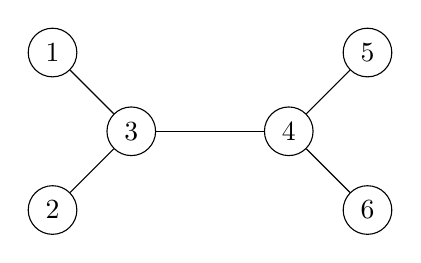
\begin{tikzpicture}
	\tikzstyle{every node}=[draw, shape=circle];

	\node (1) at (0,2) {1};
	\node (2) at (0,0) {2};
	\node (3) at (1,1) {3};
	\node (4) at (3,1) {4};
	\node (5) at (4,2) {5};
	\node (6) at (4,0) {6};

	\draw (1) -- (3);
	\draw (2) -- (3);
	\draw (3) -- (4);
	\draw (4) -- (5);
	\draw (4) -- (6);
\end{tikzpicture}
\caption{Graph of Exercise \ref{exerc:starr}} \label{fig:starr}
\end{figure}


\item \label{exerc:path} For all $q \ge 2$, determine $\guessing[D,q]$ for $D$ displayed in Figure \ref{fig:path_with_legs}.

\begin{figure}[!htp]
\centering
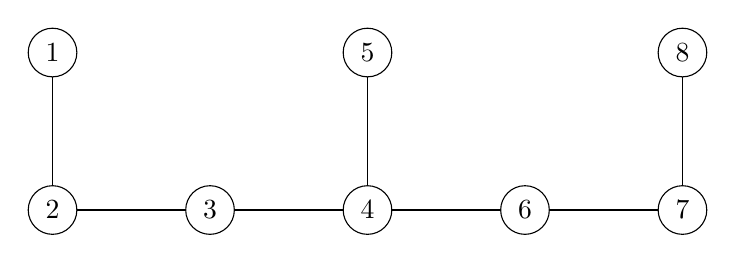
\begin{tikzpicture}
	\tikzstyle{every node}=[draw, shape=circle];

	\node (1) at (0,2) {1};
	\node (2) at (0,0) {2};
	\node (3) at (2,0) {3};
	\node (4) at (4,0) {4};
	\node (5) at (4,2) {5};
	\node (6) at (6,0) {6};
	\node (7) at (8,0) {7};
	\node (8) at (8,2) {8};

	\draw (1) -- (2);
	\draw (2) -- (3);
	\draw (3) -- (4);
	\draw (4) -- (5);
	\draw (4) -- (6);
	\draw (6) -- (7);
	\draw (7) -- (8);
\end{tikzpicture}
\caption{Graph of Exercise \ref{exerc:path}} \label{fig:path_with_legs}
\end{figure}


\item \label{exerc:star} Let $n \ge 2$. Determine $\guessing[\loopfull{iS_n}, q]$, where $iS_n$ is the inward directed star with arcs $vn$ for all $1 \le v \le n-1$. Do the same for $\loopfull{oS_n}$, where $oS_n$ is the outward directed star with arcs $nv$ for all $1 \le v \le n-1$.

\item For any $m,s \ge 1$ and $q$, determine $\guessing[\loopfull{K_{m,s}}, q]$. Keeping $n = m + s$ constant, which value of $m$ maximises the $q$-strict guessing number of $K_{m,s}$?


\item Let $n \ge 2$. Say that $D$ is $q$-fixed point universal if for any $C \subseteq \(q\)^n$, there exists $f \in \functions(D, q)$ such that $\Fix(f) = C$. Prove that the following are equivalent.
\begin{itemize}
	\item $D$ is $q$-fixed point universal for any $q$,  

	\item $D$ is $q$-fixed point universal for some $q$,
	
	\item $\feedback(D) = \dInMax(D) = n$,
	
	\item $D$ has a spanning subgraph isomorphic to $\loopfull{iS_n}$.
\end{itemize}

\item Without using Theorem \ref{th:guessing_number_feedback2}, prove that if $D$ is undirected and $\guessing(D,q) > 1$ for some $q \ge 2$, then $\guessing(D,q) \ge 2$ for all $q$.


\item Give an alternate proof of Lemma \ref{lem:g(qs)} using the guessing graph. 
%Prove that $\guessingGraph(D, qt) \subseteq \guesssingGraph(D,q) \oplus \guesssingGraph(D,t)$

\item \label{exerc:graph_products} Prove the properties of the three graph products given in Section \ref{sec:guessing_graph_graph_union}.

\item Prove that for any $D$, $k$ and $q$, $\guessingGraph(k\oplus D,q) = \guessingGraph(D,q^k)$ and hence $\guessing(k \oplus D, q) = k \guessing(D, q^k)$.

\item Draw the following guessing graphs.
\begin{exercises}
	\item Let $D = K_1 \bcup \vec{P_2}$. Then draw $\guessingGraph(D, 2)$ and $\guessingGraph(D, 3)$.
	
	\item Draw the binary guessing graph of the pentagon: $\guessingGraph(C_5,2)$. What is $\guessing(C_5, 2)$?
\end{exercises}

\item Let $f \in \functions(D,q)$ be the function with $q^{\packing(D)}$ fixed points obtained by packing cycles (see Corollary \ref{cor:g_packing}). Show that $f$ is maximal, i.e. there is no $f' \in \functions(D,q)$ with $\Fix(f') \supset \Fix(f)$.


\item \label{exerc:feedback=n-1} Prove that if $\feedback(D) = n-1$, then $\guessing(D, q) = n-1$ for all $q$. For each $n$, exhibit a graph $D$ and a graph $D'$, both on $n$ vertices and of transversal number $n-1$, such that $\guessing[D, q] < \guessing[D', q] = n-1$ for all $q$.



\item \label{exerc:metric_feedback_bound} Prove the following ``metric feedback bound:'' for any $f \in \functions(D, q)$, there are at most $q^{\feedback(D)} \VH(n-\feedback(D), q, i)$ states $x$ such that $\dH(x, f(x)) \le i$.

\item There is also an ``equivalence'' version of the feedback bound. For any code $\mathcal{C} \subseteq \(q\)^n$, an information set of $\mathcal{C}$ is a set $J \subseteq [n]$ such that for any $y \in q^J$, there is at most one codeword $x \in \mathcal{C}$ with $x_J = y$.  Prove that for any $\mathcal{C} \subseteq \(q\)^n$, $J$ is an information set of $\mathcal{C}$ if and only if there exists $f \in \functions(n,q)$ such that $J$ is a feedback vertex set of $\IG(f)$.

\item \label{exerc:solvability_is_not_local} Let $D$ be a graph on $n$ vertices and $E_n$ be the empty graph on $n$ vertices. Prove that $\guessing(D \bcup E_n, q) = n$. Therefore, for every graph $D$, there exists a solvable graph $H$ such that $D$ is an induced subgraph of $H$.

\item Which loopless graph(s) $D$ on $n$ vertices minimise(s) $\guessing[\loopfull{D}, 2]$?

\item Instead of states fixed by $f$, let us study the states increased by $f$: the states $x$ such that $f(x) \ge x$. For any $D$ and $q$, determine
the minimum, average and maximum values of $|\{ x : f(x) \ge x \}|$ for $f \in \functions[D, q]$.

\item \label{exerc:Singleton_induction1} Let us give another proof of the Singleton bound and of the feedback bound, this time by induction.
\begin{exercises}
	\item Prove that $\AH(n,q,d) \le q \AH(n-1, q, d)$ for all $n$, $q$, and $d \le n$ (with the convention that $\AH(d-1, q, d) = 1$). Deduce the Singleton bound.
	
	\item Give an analogue proof of the feedback bound.
\end{exercises}

\end{exercises}



















\chapter{Reaching the feedback bound} \label{ch:optimality_feedback}

In this chapter, we are interested in reaching the feedback bound on the guessing number. In view of the results from Chapter \ref{ch:fixed_points_unsigned}, we will mostly consider strong loopless interaction graphs, but we will give results in their full generality if that does not hurt their readability. We shall focus on reaching the feedback bound by linear functions (we introduce the linear guessing number in Section \ref{sec:gL}). As expected, the linear guessing number of a graph is the sum of the guessing numbers of its strong components, so our assumption remains valid in the linear case.

We say a graph $D$ is \BF{$q$-solvable}\index{solvable} if 
\[
	\guessing(D, q) = \feedback(D).
\]
Moreover, we say that $D$ is \BF{solvable} if it is solvable for some $q \ge 2$; we say that $D$ is \BF{all-solvable} if it is solvable for all $q \ge 2$. We similarly define strictly solvable graphs, linearly solvable graphs, etc.

The rest of the chapter is organised as follows. Firstly, we give some general results on the linear guessing number and use it to find linearly solvable graphs with interesting properties. Then, we use the reduction of FDSs to further study and classify linearly solvable graphs. Solvability is closely related to network coding, which is the topic of the last section; we then use network coding techniques to prove some strong solvability results.


\section{Linear solvability} \label{sec:linear_solvability}

In this section, we are interested in reaching the feedback bound on the guessing number by linear functions. This section is mainly taken from \cite{GR11}.

\subsection{Linear guessing number} \label{sec:gL}



Recall that the finite field $\GF(q)$ exists if and only if $q$ is a prime power, and that the set of linear functions in $\functions(n,q)$ over $\GF(q)$ is denoted as $\linearFunctions(n, q)$. The \BF{$q$-linear guessing number}\index{number!guessing!linear} of $D$ is 
\begin{align*}
	\linearGuessing(D, q) &= \max\{ \guessing(f) : f \in \linearFunctions(D,q) \} \\
	&= \max\{ \dim \Fix(f) : f \in \linearFunctions(D,q) \}.
\end{align*}
We immediately see that the linear guessing number is always an integer. Moreover, the feedback bound obviously applies to the linear guessing number:
\[
		\linearGuessing(D, q) \le \feedback(D),
\]
and we say that $D$ is \BF{$q$-linearly solvable}\index{solvable!linearly} if $\linearGuessing(D, q) = \feedback(D)$. We then say that $D$ is linearly solvable if it is $q$-linearly solvable for some prime power $q$ and that $D$ is all-linearly solvable if it $q$-linearly solvable for all prime powers $q$. We remark that if $D$ is all-linearly solvable, then it is all-solvable (i.e. solvable for all $q \ge 2$). Similarly, $D$ is $q$-strictly linearly solvable if $\linearGuessing[D,q] = \feedback(D)$; strictly linearly solvable and all-strictly linearly solvable graphs are defined accordingly. Again, if $D$ is all-strictly linearly solvable, then it is all-linearly solvable.

Taking a closer look at the lower bounds on the guessing number in Section \ref{sec:guessing_lower_bounds}, we see that the function used for the cycle ($f_v(x) = x_{v-1}$) is linear. On the other hand, the function used for the clique ($f_v(x) = - \sum_{u \ne v} x_u \mod q$) is technically not linear according to our terminology (it is linear on the ring $\Z_q$, but not on $\GF(q)$). However, it is easy to see that $f_v(x) = - \sum_{u \ne v} x_u$ in $\GF(q)$ is indeed linear according to our terminology. We thus obtain
\begin{align*}
	\linearGuessing(D, q) &\ge \packing(D),\\
	\linearGuessing(D, q) &\ge n - \cliqueCover(D).
\end{align*}
The fractional strategy in Theorem \ref{th:fractional} is not linear over $\GF(q^k)$, but only linear over the ring $\GF(q)^k$. This belongs to the class of so-called matrix-linear functions; for the sake of simplicity, we shall not consider them here.

A linear function $f$ can be represented in matrix form as $f(x) = x {\bf M}$. For a matrix ${\bf M} \in \GF(q)^{n \times n}$, the interaction graph of ${\bf M}$ is $\IG({\bf M}) = (V, E)$, where $uv \in E$ if and only if $m_{u,v} \ne 0$.  We then have 
\[
	\IG({\bf M}) = \IG(f), \qquad \text{where } f(x) = x {\bf M}.
\]
(In particular, if $q = 2$, then ${\bf M} = \adjacency(\IG({\bf M}))$.) We then define 
\begin{align*}
	\matrices(D,q) &:= \{ {\bf M} \in \GF(q)^{n \times n} : \IG({\bf M}) \subseteq D \},\\
	\matrices[D,q] &:= \{ {\bf M} \in \GF(q)^{n \times n} : \IG({\bf M}) = D \}.
\end{align*}
In particular, $\matrices[D, 2]$ only contains the adjacency matrix of $D$.




\begin{proposition} \label{prop:linear_guessing_rank}
For any $D$ and $q$,
\[
	\linearGuessing[D,q] = \max \{ n - \rank({\bf I} - {\bf M}) : {\bf M} \in \matrices[D, q] \}.
\]
\end{proposition}

\begin{proof}
For $f(x) = x {\bf M}$, we have $x \in \Fix(f)$ if and only if $x ({\bf I} - {\bf M}) = 0$. Therefore, $\guessing(f) = \dim \Fix(f) = n - \rank({\bf I} - {\bf M})$.
\end{proof}


\begin{corollary} \label{cor:linear_guessing_2}
For any $D$,
\[
	\linearGuessing[D, 2] = n - \rank({\bf I} + \adjacency(D)).
\]
\end{corollary}




For any graph $D = (V, E)$, let the \BF{transpose}\index{graph!transpose} of $D$ be the graph obtained by reversing the direction of all the arcs in $D$: $D^\top = (V, E^\top)$ where $uv \in E^\top$ if and only if $vu \in E$. Clearly, $\feedback(D^\top) = \feedback(D)$ and $\packing(D^\top) = \packing(D)$; also, the terminology and notation are tailored so that
$\adjacency(D)^\top = \adjacency(D^\top)$.

\begin{corollary} \label{cor:linear_guessing_transpose}
For any $D$ and $q$,
\[
	\linearGuessing[D, q] = \linearGuessing[D^\top, q].
\]
Hence, $D$ is $q$-strictly linearly solvable if and only if $D^\top$ is $q$-strictly linearly solvable.
\end{corollary}



The following is the analogue of Corollary \ref{cor:sum_strongly_connected}.

\begin{proposition} \label{prop:gl_strong}
Let $D$ be a graph with strong components $S_1, \dots, S_k$, then
\[
	\linearGuessing(D,q) = \sum_{i=1}^k \linearGuessing(S_i, q).
\]
\end{proposition}


\begin{proof} \renewcommand*{\arraystretch}{1.5}
We only need to prove that for any two graphs $D_1$ and $D_2$ with disjoint vertex sets $V_1$ and $V_2$, we have
\[
	\linearGuessing(D_1 \vcup D_2, q) = \linearGuessing(D_1 \cup D_2, q) = \linearGuessing(D_1, q) + \linearGuessing(D_2, q).
\]
It is clear that $\linearGuessing(D_1 \vcup D_2, q) \ge  \linearGuessing(D_1, q) + \linearGuessing(D_2, q)$, we thus show the reverse inequality.


For any ${\bf M} \in \matrices(D_1 \vcup D_2, q)$, we have
\[
	{\bf I}_n - {\bf M} = \left(\begin{array}{c|c}
	{\bf I}_{n_1} - {\bf M}_1 & {\bf M}_3\\
	\hline
	{\bf 0} & {\bf I}_{n_2} - {\bf M}_2
	\end{array}\right),
\]
where ${\bf M}_1 \in \matrices(D_1, q)$ and ${\bf M}_2 \in \matrices(D_2, q)$. Therefore,
\begin{align*}
	\rank({\bf I}_n - {\bf M}) &\ge \rank({\bf I}_{n_1} - {\bf M}_1) + \rank({\bf I}_{n_2} - {\bf M}_2)\\
	&\ge \left\{n_2 - \linearGuessing(D_1, q) \right\} + \left\{ n_1 - \linearGuessing(D_2, q) \right\},
\end{align*}
and hence $\linearGuessing(D_1 \vcup D_2, q) \le \linearGuessing(D_1, q) + \linearGuessing(D_2, q)$.
\end{proof}


The linear guessing number of the bidirectional union behaves especially well.

\begin{proposition} \label{prop:gl_bidirectional}
For any $D_1$ and $D_2$ on disjoint vertex sets and any $q$,
\[
	\linearGuessing(D_1 \bcup D_2, q) = \min\{ \linearGuessing(D_1, q) + n_2, \linearGuessing(D_2, q) + n_1 \}.
\]
\end{proposition}

\begin{proof} \renewcommand*{\arraystretch}{1.5}
For any ${\bf M} \in \matrices(D_1 \bcup D_2, q)$, we have
\[
	{\bf I}_n - {\bf M} = \left(\begin{array}{c|c}
	{\bf I}_{n_1} - {\bf M}_1 & {\bf M}_3\\
	\hline
	{\bf M}_4 & {\bf I}_{n_2} - {\bf M}_2
	\end{array}\right),
\]
where ${\bf M}_1 \in \matrices(D_1, q)$ and ${\bf M}_2 \in \matrices(D_2, q)$. Therefore,
\[
	\rank({\bf I}_n - {\bf M}) \ge \rank({\bf I}_{n_1} - {\bf M}_1),
\]
and hence $\linearGuessing(D_1 \bcup D_2, q) \le \linearGuessing(D_1, q) + n_2$. Similarly, we obtain $\linearGuessing(D_1 \bcup D_2, q) \le \linearGuessing(D_2, q) + n_1$.

Conversely, without loss suppose $l = n_1 - \linearGuessing(D_1, q) \ge n_2 - \linearGuessing(D_2, q)$ and let ${\bf M}_i \in \matrices(D_i, q)$ satisfy $\rank({\bf I}_{n_i} - {\bf M}_i) = n_i - \linearGuessing(D_i, q)$ for $i = 1,2$. We can express ${\bf N}_i = {\bf I}_{n_i} - {\bf M}_i$ as ${\bf N}_i = {\bf B}_i^\top {\bf C}_i$, where ${\bf B}_i, {\bf C}_i \in \GF(q)^{l \times n_i}$. Then the matrix 
\[
	{\bf N} := \left(\begin{array}{c} 
	{{\bf B}_1^\top}\\
	\hline
	{{\bf B_2}^\top}
	\end{array}\right)
	\left( \begin{array}{c|c}
	{\bf C}_1 & {\bf C}_2
	\end{array} \right)
	= \left( \begin{array}{c|c}
	{\bf N}_1 & {\bf B}_1^\top {\bf C}_2\\
	\hline
	{\bf B}_2^\top {\bf C}_1 & {\bf N}_2
	\end{array} \right)
\]
has rank $l$ and the interaction graph of ${\bf M} = {\bf N} - {\bf I}$ is contained in $D_1 \bcup D_2$.
\end{proof}






\subsection{Linearly solvable graphs from cyclic codes} \label{sec:linearly_solvable_cyclic_codes}



If $f$ is linear, say $f(x) = x {\bf M}$, then $\Fix(f)$ is an $(n,k)_q$ linear code, where $k$ is the guessing number of $f$. This code is defined by
\[
	\Fix(f) = \{ x \in \GF(q)^n : x ({\bf I}_n - {\bf M}) = 0 \}.
\]
This is reminiscent of the definition of any linear code $\mathcal{C}$ by its parity-check matrix:
\[
	\mathcal{C} = \{ x \in \GF(q)^n : x {\bf H}^\top = 0 \}.
\]
The main difference is that ${\bf H}$ has $n-k$ linearly independent rows, while $({\bf I}_n - {\bf M})^\top$ has $n$ rows which are not necessarily linearly independent (in fact, we want the rank of that matrix to be as low as possible). This can be remedied as such: if we take ${\bf H}$ and append linear combinations of its rows, then we obtain a square matrix $\hat{\bf H}$ such that 
\[
	\mathcal{C} = \{ x \in \GF(q)^n : x \hat{\bf H}^\top = 0 \}.
\]

The paragraph above indicates a general strategy to design graphs with interesting guessing number properties:
\begin{enumerate}
	\item take a ``good'' parity-check matrix ${\bf H}$ of an $(n,k)_q$ linear code;
	
	\item append linear combinations of its rows to obtain $\hat{\bf H}$;
	
	\item let $D$ be the interaction graph of the matrix $({\bf I}_n - \hat{\bf H}^\top)^\top = {\bf I}_n - \hat{\bf H}$.
\end{enumerate}
Then immediately we have $\linearGuessing[D,q] \ge n-k$.

In this section, we give a strategy, based on cyclic codes, to select the parity-check matrix ${\bf H}$ and construct the matrix $\hat{\bf H}$ in order to produce linearly solvable graphs.


An $(n,k)_q$ linear code $\mathcal{C}$ is \BF{cyclic}\index{code!cyclic} if for every codeword $x = (x_1, x_2, \dots, x_n) \in \mathcal{C}$, its cyclic shift $x' = (x_n, x_1, \dots, x_{n-1})$ is also in $\mathcal{C}$. The key to understand cyclic codes is by viewing each codeword $x$ as a polynomial:
\begin{align*}
	c(\xi) &:= x_1 + x_2 \xi + \dots + x_n \xi^{n-1}\\
	&= c_0 + c_1 \xi + \dots + c_{n-1} \xi^{n-1}.
\end{align*}
Then the cyclic shift corresponds to multiplying by $\xi \mod (\xi^n-1)$:
\[
	\xi c(\xi) = c'(\xi) \mod (\xi^n - 1).
\]
We hence place ourselves in $\GF(q)[\xi] / (\xi^n - 1)$. Let $c(\xi)$ be a codeword in $\mathcal{C}$, then 
\[
	\xi c(\xi), \quad \xi^2 c(\xi), \quad \dots, \quad \xi^{n-1} c(\xi), \quad \xi^n c(\xi) = c(\xi) \in \mathcal{C}.
\]
Since the code is linear, we obtain that for any $a(\xi)$, $a(\xi)c(\xi) \in \mathcal{C}$. Thus $\mathcal{C}$ is an ideal of $\GF(q)[\xi] / (\xi^n - 1)$. This in fact characterises cyclic codes: $\mathcal{C}$ is a $q$-ary cyclic code of length $n$ if and only if the code polynomials form an ideal in $\GF(q)[\xi] / (\xi^n - 1)$.

Let us enumerate some properties of cyclic codes; the proofs can be found in \cite{MS77}. Let $\mathcal{C}$ be an $(n,k)_q$ cyclic code.
\begin{enumerate}
	\item There exists a unique monic polynomial $g(\xi)$ in the code with minimal degree $r = n-k$. $g(\xi)$ is the \BF{generator polynomial}\index{polynomial!generator} of $\mathcal{C}$.

	\item \label{it:g_divides_xn-1} $g(\xi)$ is a factor of $\xi^n - 1$ in $\GF(q)[\xi]$.
	
	\item Every code polynomial $c(\xi) \in \mathcal{C}$ can be expressed uniquely as 
	\[
		c(\xi) = m(\xi) g(\xi),
	\]
	where $m(\xi)$ is the message polynomial, of degree $\deg m(\xi) < k$.
	

	\item The generator matrix of $\mathcal{C}$ with generator polynomial $g(\xi) = \sum_{i=0}^r g_i \xi^i$ is
	\[
		{\bf G} = \begin{pmatrix}
		g_0		& g_1	& \dots 	& g_r 		& 			& 			& 		& {\bf 0}\\
				& g_0	& g_1 		& \dots 	& g_r 		& 			& 		& \\
				&    	& \ddots 	& \ddots 	& \ddots 	& \ddots 	& 		& \\
				& 		& 			& g_0		& g_1		& \dots		& g_r	& \\
		{\bf 0}	& 		& 			&			& g_0		& g_1		& \dots	& g_r 
		\end{pmatrix}.
	\]

Indeed, $c(\xi) = m(\xi) g(\xi)$ corresponds to $c = m {\bf G}$.
\end{enumerate}


The parity-check matrix is also easy to determine. By Property \ref{it:g_divides_xn-1}, there exists a polynomial $h(\xi) = \sum_{i=0}^k h_i \xi^i \in \GF(q)[\xi]$ such that
\[
	g(\xi)h(\xi) = \xi^n - 1 \quad \text{in } \GF(q)[\xi].
\]
Then $c(\xi) \in \mathcal{C}$ if and only if
\[
	c(\xi) h(\xi) = 0 \quad \text{in } \GF(q)[\xi] / (\xi^n - 1).
\]
In matrix form, this is equivalent to $c {\bf H}^\top = 0$, where
\[
	{\bf H} = \begin{pmatrix}
	h_k		& \dots	& h_1 		& h_0		& 			& 			& {\bf 0}\\
			& h_k	& \dots		& h_1	 	& h_0 		& 			& 		& \\
			&    	& \ddots 	& \ddots 	& \ddots 	& \ddots 	& 		& \\
			& 		& 			& h_k		& \dots		& h_1		& h_0	& \\
	{\bf 0}	& 		& 			&			& h_k		& \dots		& h_1	& h_0 
	\end{pmatrix}.
\]
In polynomial form, we see that for any $f(\xi) = \sum_{i=0}^d f_i \xi^i$ of degree $d$, its \BF{reciprocal} is
\[
	f^*(\xi) := \xi^d f(\xi^{-1}) = \sum_{i=0}^d f_{d-i} \xi^i.
\]
We have obtained: if $\mathcal{C}$ is the cyclic code generated by $g(\xi)$, then $\mathcal{C}^\perp$ is the cyclic code generated by $h^*(\xi)$, the reciprocal of the parity polynomial of $\mathcal{C}$. Therefore, we can extend the parity-check matrix as such:
\[
	\hat{\bf H} = \begin{pmatrix}
	h^*(\xi)\\
	\xi h^*(\xi)\\
	\vdots\\
	\xi^{n-1} h^*(\xi)
	\end{pmatrix},
\]
and this matrix has rank $n - k$ and ones all over the diagonal.


Since we aim to construct graphs based on the parity-check matrix of a code, we shall focus on $h^*(\xi)$. Without loss, we assume that $h^*(\xi) = h_k + h_{k-1} \xi + \dots + h_0 \xi^k$, with $h_k = 1$ if $h^*$ is non-zero. We say that $h^*(\xi)$ produces $\mathcal{C}$; moreover the graph $D_{h^*}$ produced by $h^*$ is the interaction graph of the matrix ${\bf I}_n - \hat{\bf H}$.





\begin{example} \label{ex:trivial_cyclic_graphs}
The polynomial $\xi^n - 1$ has two trivial factorisations:
\[
	\xi^n - 1 = (1)(\xi^n-1) = (\xi-1)(\xi^{n-1} + \xi^{n-2} + \dots + 1).
\]
The four terms produce famous cyclic codes and graphs. We use $n = 4$ as illustration.
\begin{itemize}
    \item The polynomial $h^*(\xi) = 1$ produces the subspace of dimension zero and the empty graph:
	\[
		{\bf H} = \begin{pmatrix}
		1 & 0 & 0 & 0\\
		0 & 1 & 0 & 0\\
		0 & 0 & 1 & 0\\
		0 & 0 & 0 & 1
		\end{pmatrix}, \qquad
		\hat{\bf H} = \begin{pmatrix}
		1 & 0 & 0 & 0\\
		0 & 1 & 0 & 0\\
		0 & 0 & 1 & 0\\
		0 & 0 & 0 & 1
		\end{pmatrix}, \qquad
		\adjacency(D_{h^*}) = \begin{pmatrix}
		0 & 0 & 0 & 0\\
		0 & 0 & 0 & 0\\
		0 & 0 & 0 & 0\\
		0 & 0 & 0 & 0
		\end{pmatrix}.
	\]

    \item The polynomial $h^*(\xi) = -\xi + 1$ produces the repetition code and the cycle $\vec{C}_n$:
	\[
		{\bf H} = \begin{pmatrix}
		1 & -1 & 0 & 0\\
		0 & 1 & -1 & 0\\
		0 & 0 & 1 & -1
		\end{pmatrix}, \qquad
		\hat{\bf H} = \begin{pmatrix}
		1 & -1 & 0 & 0\\
		0 & 1 & -1 & 0\\
		0 & 0 & 1 & -1\\
		-1 & 0 & 0 & 1
		\end{pmatrix}, \qquad
		\adjacency(D_{h^*}) = \begin{pmatrix}
		0 & 1 & 0 & 0\\
		0 & 0 & 1 & 0\\
		0 & 0 & 0 & 1\\
		1 & 0 & 0 & 0
		\end{pmatrix}.
	\]

    \item The polynomial $h^*(\xi) = \xi^{n-1} + \xi^{n-2} + \dots + 1$ produces the parity-check code and the clique $K_n$:
	\[
		{\bf H} = \begin{pmatrix}
		1 & 1 & 1 & 1
		\end{pmatrix}, \qquad
		\hat{\bf H} = \begin{pmatrix}
		1 & 1 & 1 & 1\\
		1 & 1 & 1 & 1\\
		1 & 1 & 1 & 1\\
		1 & 1 & 1 & 1
		\end{pmatrix}, \qquad
		\adjacency(D_{h^*}) = \begin{pmatrix}
		0 & 1 & 1 & 1\\
		1 & 0 & 1 & 1\\
		1 & 1 & 0 & 1\\
		1 & 1 & 1 & 0
		\end{pmatrix}.
	\]
	
	
	\item The polynomial $h^*(\xi) = \xi^n - 1$ is equal to $0$ modulo $\xi^n-1$; as such it produces the whole space $\GF(q)^n$ and the empty graph with a loop on each vertex:
	\[
		{\bf H} = \begin{pmatrix}
		0 & 0 & 0 & 0
		\end{pmatrix}, \qquad
		\hat{\bf H} = \begin{pmatrix}
		0 & 0 & 0 & 0\\
		0 & 0 & 0 & 0\\
		0 & 0 & 0 & 0\\
		0 & 0 & 0 & 0
		\end{pmatrix}, \qquad
		\adjacency(D_{h^*}) = \begin{pmatrix}
		1 & 0 & 0 & 0\\
		0 & 1 & 0 & 0\\
		0 & 0 & 1 & 0\\
		0 & 0 & 0 & 1
		\end{pmatrix}.
	\]
\end{itemize}
\end{example}

All the graphs in the previous example are strictly linearly solvable. Theorem \ref{th:graph_produced_by_code} shows that this is always the case.


\begin{theorem} \label{th:graph_produced_by_code}
For any $n$ and any polynomial $h^*(\xi) \in \GF(q)[\xi]$ dividing $\xi^n - 1$, the graph $D_{h^*}$ is in- and out-regular with degree $\wH(h^*) - 1$ and is strictly linearly solvable over $\GF(q)$, where
\[
	\linearGuessing[D_{h^*}, q] = \feedback(D_{h^*}) = \deg(h^*).
\]
\end{theorem}


\begin{proof}
The degree of a vertex in $D_{h^*}$ follows from the construction. Let $k = \deg(h^*)$, then by construction, 
\[
	\linearGuessing[D_{h^*}, q] \ge n - \rank({\bf I}_n - \adjacency(D_{h^*})) = n - \rank(\hat{\bf H}) = k.
\]
Conversely, the first $n-k$ rows and $n-k$ columns of $\adjacency(D_{h^*})$ are
\[
	\begin{pmatrix}
	0		& \dots	& h_1 		& h_0		\\
			& 0 	& \dots		& h_1	 	\\
			&    	& \ddots 	& \ddots 	\\
	{\bf 0}	& 		& 			& 0		
	\end{pmatrix},
\]
hence the first $n-k$ vertices form an acyclic set, and $\feedback(D) \le k$.
\end{proof}


We finish this part with a non-trivial example of graph produced by a polynomial: the Paley tournament on seven vertices.

\begin{example}[The Paley tournament on seven vertices] \label{ex:Paley}
Let $q=2$, $n=7$ and $h^*(\xi) = \xi^4 + \xi^2 + \xi + 1$. This generates a code equivalent to the Hamming code of length $7$ (see Section \ref{sec:coding_theory}). Then the graph $\mathrm{Paley} = D_{h^*}$ satisfies
\[
	\adjacency(\mathrm{Paley}) = \begin{pmatrix}
		0 & 1 & 1 & 0 & 1 & 0 & 0 \\
		0 & 0 & 1 & 1 & 0 & 1 & 0 \\
		0 & 0 & 0 & 1 & 1 & 0 & 1 \\
		1 & 0 & 0 & 0 & 1 & 1 & 0 \\
		0 & 1 & 0 & 0 & 0 & 1 & 1 \\
		1 & 0 & 1 & 0 & 0 & 0 & 1 \\
		1 & 1 & 0 & 1 & 0 & 0 & 0 
		\end{pmatrix}.
\]
We have $\linearGuessing[\mathrm{Paley}, 2] = \feedback(\mathrm{Paley}) = 4$, which is higher than the lower bounds on the linear guessing number obtained from packing cycles or cliques: $\packing(\mathrm{Paley}) = 2$ and $n - \cliqueCover(\mathrm{Paley}) = 0$. 
\end{example}


\begin{figure}
\centering
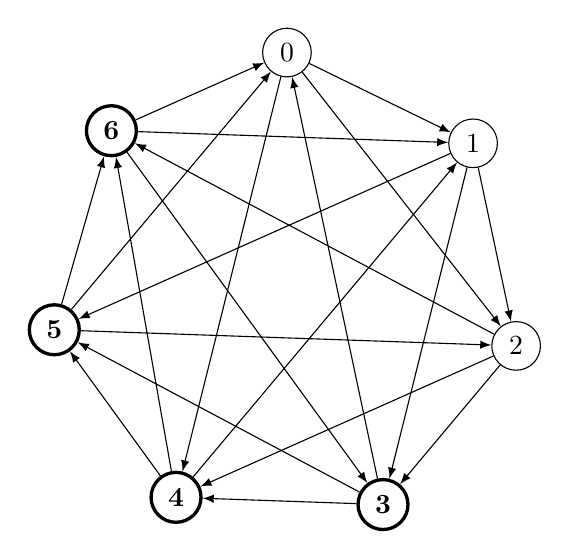
\begin{tikzpicture}
\tikzstyle{every node}=[draw, shape=circle];

\foreach \x in {3,...,6}{
	\node[very thick] (\x) at (90-52*\x:3) {${\bf \x}$};
}
\foreach \x in {0,1,2}{
	\node (\x) at (90-52*\x:3) {\x};
}

	\draw[-latex] (0) -- (1);
	\draw[-latex] (0) -- (2);
	\draw[-latex] (0) -- (4);
	
	\draw[-latex] (1) -- (2);
	\draw[-latex] (1) -- (3);
	\draw[-latex] (1) -- (5);

	\draw[-latex] (2) -- (3);
	\draw[-latex] (2) -- (4);
	\draw[-latex] (2) -- (6);
	
	\draw[-latex] (3) -- (4);
	\draw[-latex] (3) -- (5);
	\draw[-latex] (3) -- (0);

	\draw[-latex] (4) -- (5);
	\draw[-latex] (4) -- (6);
	\draw[-latex] (4) -- (1);
	
	\draw[-latex] (5) -- (6);
	\draw[-latex] (5) -- (0);
	\draw[-latex] (5) -- (2);

	\draw[-latex] (6) -- (0);
	\draw[-latex] (6) -- (1);
	\draw[-latex] (6) -- (3);
\end{tikzpicture}
\caption{The Paley tournament on $7$ vertices produced by $\xi^4 + \xi^2 + \xi + 1$ with binary linear guessing number $4$.}
\label{fig:P7}
\end{figure}






\subsection{Sparse linearly solvable graphs} \label{sec:sparse_linearly_solvable}


We are now interested in constructing graphs $D$ which are sparse (i.e., relatively low maximal in- and out-degree) and yet which have a high guessing number, say $\guessing(D) = (1 - o(1))n$. Let $\hat{\gamma}, \hat{\Delta} : \N^+ \to \N^+$ be two functions indicating the girth and the sparsity of our graphs. We say that a sequence of graphs $\{D_k\}_{k \ge 1}$ on $n_k := |V(D_k)|$ vertices is \BF{$(\hat{\gamma}, \hat{\Delta})$-suitable}\index{suitable sequence of graphs} if they satisfy the following three properties for all $k \ge 1$:
\begin{align*}
	\girth(D_k) &\ge \hat{\gamma}(n_k),\\
	\dInMax(D_k) + \dOutMax(D_k) &\le \hat{\Delta}(n_k),\\
	\linearGuessing[D_k, q] &= \feedback(D_k) \quad \forall q,\\
	\lim_{k \to \infty} \frac{\feedback(D_k)}{n_k} &= 1.
\end{align*}
In other words, these graphs are sparse, all-strictly linearly solvable and their guessing number is asymptotically equivalent to the number of vertices. 

For $\hat{\gamma} = 1$, this can be trivially achieved: let $L_n$ be the graph with only $n$ loops, then
\[
	\dInMax(L_n) = \dOutMax(L_n) = 1, \qquad \linearGuessing[L_n, q] = \feedback(L_n) = n.
\]
If we require that $\hat{\gamma}(n) \ge 2$ for all $n$ large enough, i.e. that almost all the graphs in the sequence are loopless, then we have two constraints on $\hat{\gamma}$ and $\hat{\Delta}$.
\begin{enumerate}
	\item Since $\feedback(D) \le n - \girth(D) + 1$ for any graph $D$, we have $\hat{\gamma} = o(n)$. We shall restrict ourselves to constant $\hat{\gamma}$ from now on. In that case, when $\hat{\gamma}$ is fixed and $k$ tends to infinity, the ratio between $\feedback(D_k)$ and $\packing(D_k)$ is at least $\hat{\gamma} - o(1)$.
	
	\item By Exercise \ref{exerc:independence_max_degree}, $\hat{\Delta}$ must be unbounded.
\end{enumerate}



The aim of this section is to prove that suitable sequences do exist.

\begin{theorem} \label{th:high_girth_g}
For any $\hat{\gamma} \ge 2$ and any unbounded function $\hat{\Delta} : \N \to \N$ , there exists a $(\hat{\gamma}, \hat{\Delta})$-suitable sequence of graphs.
\end{theorem}



First of all, constructing $(2, \hat{\Delta})$-suitable sequences of graphs is easy.

\begin{proposition} \label{prop:sparse_high_g}
For any unbounded function $\hat{\Delta} : \N^+ \to \N^+$, there exists a $(2, \hat{\Delta})$-suitable sequence of graphs.
\end{proposition}

\begin{proof}
Let $n_1 := \min\{n : \hat{\Delta}(n) \ge 2\}$ and for any $k \ge 2$, let 
\[
	n_k := \min\{ n : n \ge n_{k-1}, n \ge k(k-1), \hat{\Delta}(n) \ge 2(k-1) \}.
\]
Let $D_k$ be the disjoint union of $m := \lfloor n_k/k \rfloor$ cliques $K_k$ along with some remaining isolated vertices. Then for any $q$,
\begin{align*}
	\girth(D_k) &= 2,\\
	\dInMax(D_k) + \dOutMax(D_k) &= 2(k-1) \le \hat{\Delta}(n_k),\\
	\linearGuessing[D_k, q] = \feedback(D_k) &= m(k-1) > \left( \frac{n_k}{k} - 1 \right)(k-1) \ge n_k \left(1 - \frac{2}{k} \right).
\end{align*}
\end{proof}


Our aim is then to construct $(\hat{\gamma}, \hat{\Delta})$-suitable sequences of graphs for any fixed $\hat{\gamma} \ge 3$. We shall use the code-based approach above and combine it with the strong product of graphs. The \BF{strong product}\index{strong product} of two loopless graphs $D_1 = (V_1, E_1)$ and $D_2 = (V_2, E_2)$, denoted as $D_1 \boxtimes D_2$, has vertex set $V_1 \times V_2$ and $(u_1, u_2) (v_1, v_2)$ is an arc if and only if
\[
	u_1 = v_1, u_2v_2 \in E_1, \quad \text{ or } u_2 = v_2, u_1v_1 \in E_2, \quad \text{ or } u_1v_1 \in E_1, u_2v_2 \in E_2.
\]
Equivalently, the adjacency matrix of the strong product satisfies
\[
	{\bf I}_{n_1n_2} + \adjacency(D_1 \boxtimes D_2) = ({\bf I}_{n_1} + \adjacency(D_1)) \otimes ({\bf I}_{n_2} + \adjacency(D_2)),
\]
where $\otimes$ denotes the Kronecker product of matrices. For instance, the graph $\vec{C}_3 \boxtimes \vec{C}_3$ is illustrated in Figure \ref{fig:C32}. Its adjacency matrix is
\[
	\adjacency(D_1 \boxtimes D_2) = \left( \begin{array}{ccc|ccc|ccc}
	0 & 1 & 0 & 1 & 1 & 0 & 0 & 0 & 0\\
	0 & 0 & 1 & 0 & 1 & 1 & 0 & 0 & 0\\
	1 & 0 & 0 & 1 & 0 & 1 & 0 & 0 & 0\\
	\hline
	0 & 0 & 0 & 0 & 1 & 0 & 1 & 1 & 0\\
	0 & 0 & 0 & 0 & 0 & 1 & 0 & 1 & 1\\
	0 & 0 & 0 & 1 & 0 & 0 & 1 & 0 & 1\\
	\hline
	1 & 1 & 0 & 0 & 0 & 0 & 0 & 1 & 0\\
	0 & 1 & 1 & 0 & 0 & 0 & 0 & 0 & 1\\
	1 & 0 & 1 & 0 & 0 & 0 & 1 & 0 & 0
	\end{array} \right).
\]

Some properties of the strong product are listed below (their proofs are asked in Exercise \ref{exerc:strong_product}). 

\begin{proposition} \label{prop:strong_product}
The strong product $D_1 \boxtimes D_2$ satisfies the following properties.
\begin{enumerate}
	\item \label{it:strong_product_girth} The girth of $D_1 \boxtimes D_2$ is given by
	\[
		\girth(D_1 \boxtimes D_2) = \min\{ \girth(D_1), \girth(D_2) \}.
	\]
		
	\item If $D_1$ and $D_2$ are in-regular, then so is $D_1 \boxtimes D_2$, and
	\[
		\dIn(D_1 \boxtimes D_2) + 1 = (\dIn(D_1) + 1) (\dIn(D_2) + 1).
	\]
	The same result holds for out-regular graphs.
	
	\item The transversal number of $D_1 \boxtimes D_2$ is given by
	\[
		n_1n_2 - \feedback(D_1 \boxtimes D_2) = (n_1 - \feedback(D_1)) (n_2 - \feedback(D_2)).
	\]
	
	\item The linear guessing number of $D_1 \boxtimes D_2$ satisfies
	\[
		n_1n_2 - \linearGuessing(D_1 \boxtimes D_2, q) \le (n_1 - \linearGuessing(D_1, q)) (n_2 - \linearGuessing(D_2, q)).
	\]
	A similar result holds for the strict linear guessing number (with equality for $q=2$).
\end{enumerate}
\end{proposition}

%\begin{proof}
%We let $D = D_1 \boxtimes D_2$ and $n = n_1n_2$.
%
%\ref{it:strong_product_girth}. Firstly, for any $v_1 \in V_1$ and any $v_2^1, v_2^2, \dots, v_2^k \in V_2$ forming a cycle in $D_2$, the vertices $(v_1, v_2^1), (v_1, v_2^2), \dots, (v_1, v_2^k)$ form a cycle in $D$. A similar result holds for any $v_2 \in V_2$ and any cycle in $D_1$. Hence $\girth(D) \le \min\{ \girth(D_1), \girth(D_2) \}$. Conversely, suppose $(v_1^1, v_2^1), \dots, (v_1^k, v_2^k)$ form a cycle in $D$. Suppose there exists $i$ such that $v_1^i \ne v_1^1$, then after removing repetitions, the vertices $v_1^1, \dots, v_1^k$ form a cycle of $D_1$ and $k \ge \girth(D_1)$. The same argument holds for $D_2$, and we obtain $\girth(D) \ge \min\{ \girth(D_1), \girth(D_2) \}$.
%
%\ref{it:strong_product_degree} follows from the definition.
%
%\ref{it:strong_product_feedback} follows from the arguments for the girth.
%
%\ref{it:strong_product_linear_guessing} follows from the rank of the Kronecker product of matrices.
%\end{proof}

\begin{corollary}
If $D_1$ and $D_2$ are $q$-strictly linearly solvable, then so is $D_1 \boxtimes D_2$.
\end{corollary}


We can now choose a graph and repeatedly take the strong product of the graph with itself. Out of the four graphs in Example \ref{ex:trivial_cyclic_graphs}, only one is interesting. For any $k \ge 1$ and $\hat{\gamma} \ge 3$, denote the cycle $\vec{C}_{\hat{\gamma}}$ raised to the power $k$ according to the strong product as $\vec{C}_{\hat{\gamma}}^k$. Then $\vec{C}_{\hat{\gamma}}^k$ has the following properties:
\begin{enumerate}
	\item it has $n_{\hat{\gamma},k} = \hat{\gamma}^k$ vertices,
	
	\item it is an in- and out-regular of degree $d_{\hat{\gamma},k} = 2^k - 1$,
	
	\item its girth is $\hat{\gamma}$,
	
%	\item its packing number is $\nu_{\hat{\gamma}, k} = \hat{\gamma}^{k-1}$,
	
	\item its transversal number is $\feedback_{\hat{\gamma}, k} = \hat{\gamma}^k - (\hat{\gamma} - 1)^k$,
	
	\item it is strictly linearly solvable over all finite fields, i.e. $\linearGuessing[\vec{C}_{\hat{\gamma}}^k, q] = \hat{\gamma}^k - (\hat{\gamma} - 1)^k$.
\end{enumerate}
By using the same disjoint union technique as in Proposition \ref{prop:sparse_high_g}, but this time with the graphs $\vec{C}_{\hat{\gamma}}^k$, we obtain Theorem \ref{th:high_girth_g}.



\begin{figure}
\centering
	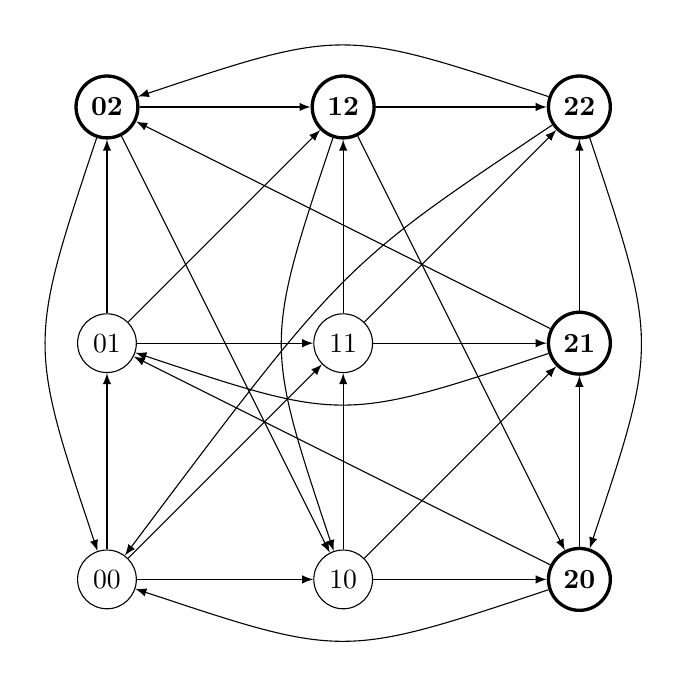
\begin{tikzpicture}
	\tikzstyle{every node}=[draw, shape = circle];
	
	\node (00) at (0,0) {00};
	\node (01) at (0,3) {01};
	\node[very thick] (02) at (0,6) {${\bf 02}$};
	\node (10) at (3,0) {10};
	\node (11) at (3,3) {11};
	\node[very thick] (12) at (3,6) {${\bf 12}$};
	\node[very thick] (20) at (6,0) {${\bf 20}$};
	\node[very thick] (21) at (6,3) {${\bf 21}$};
	\node[very thick] (22) at (6,6) {${\bf 22}$};
	
	\draw[-latex] (00) -- (01);
	\draw[-latex] (00) -- (10);
	\draw[-latex] (00) -- (11);
	
	\draw[-latex] (01) -- (02);
	\draw[-latex] (01) -- (11);
	\draw[-latex] (01) -- (12);
	
	%\draw[-latex] (02) -- (00);
	\draw[-latex] (02) .. controls(-1,3) .. (00);
	\draw[-latex] (02) -- (12);
	\draw[-latex] (02) -- (10);
	
	\draw[-latex] (10) -- (11);
	\draw[-latex] (10) -- (20);
	\draw[-latex] (10) -- (21);
	
	\draw[-latex] (11) -- (12);
	\draw[-latex] (11) -- (21);
	\draw[-latex] (11) -- (22);
	
	%\draw[-latex] (12) -- (10);
	\draw[-latex] (12) .. controls(2,3) .. (10);
	\draw[-latex] (12) -- (22);
	\draw[-latex] (12) -- (20);
	
	\draw[-latex] (20) -- (21);
	%\draw[-latex] (20) -- (00);
	\draw[-latex] (20) .. controls(3,-1) .. (00);
	\draw[-latex] (20) -- (01);
	
	\draw[-latex] (21) -- (22);
	%\draw[-latex] (21) -- (01);
	\draw[-latex] (21) .. controls(3,2) .. (01);
	\draw[-latex] (21) -- (02);
	
	%\draw[-latex] (22) -- (20);
	\draw[-latex] (22) .. controls(7,3) .. (20);
	%\draw[-latex] (22) -- (02);
	\draw[-latex] (22) .. controls(3,7) .. (02);
	%\draw[-latex] (22) -- (00);
	\draw[-latex] (22) .. controls(3,4) .. (00);
	
	\end{tikzpicture}
\caption{The graph $\vec{C}_3^2$, with linear guessing number $5$.}
\label{fig:C32}
\end{figure}












%\appendix

\cleardoublepage
\addcontentsline{toc}{chapter}{Index}
\printindex

%\bibliographystyle{plain}
%\bibliography{FDS}


\begin{thebibliography}{100}

\bibitem{SLV10}
R.~Laubenbacher A.~Salam~Jarrah and A.~Veliz-Cuba.
\newblock The dynamics of conjunctive and disjunctive boolean network models.
\newblock {\em Bulletin of Mathematical Biology}, 72:1425--1447, 2010.



\bibitem{AVZ00}
Erik Agrell, Alexander Vardy, and Kenneth Zeger.
\newblock Upper bounds for constant-weight codes.
\newblock {\em IEEE Transactions on Information Theory}, 46(7):2373--2395,
  November 2000.

\bibitem{ACLY00}
R.~Ahlswede, N.~Cai, S.-Y.~R. Li, and R.~W. Yeung.
\newblock Network information flow.
\newblock {\em IEEE Transactions on Information Theory}, 46(4):1204--1216, July
  2000.

\bibitem{A85}
Noga Alon.
\newblock Asynchronous threshold networks.
\newblock {\em Graphs and Combinatorics}, 1(1):305--310, 1985.

\bibitem{ARS14}
J.~Aracena, A.~Richard, and L.~Salinas.
\newblock Maximum number of fixed points in and-or-not networks.
\newblock {\em Journal of Computer and System Sciences}, 80(7):1175 -- 1190,
  2014.

\bibitem{Ara08}
Julio Aracena.
\newblock Maximum number of fixed points in regulatory {B}oolean networks.
\newblock {\em Bulletin of mathematical biology}, 70:1398--1409, 2008.

\bibitem{ADG04}
Julio Aracena, Jacques Demongeot, and Eric Goles.
\newblock Positive and negative circuits in discrete neural networks.
\newblock {\em IEEE Transactions on Neural Networks}, 15(1):77--83, January
  2004.

\bibitem{ARS17}
Julio Aracena, Adrien Richard, and Lilian Salinas.
\newblock Number of fixed points and disjoint cycles in monotone boolean
  networks.
\newblock {\em accepted in SIAM journal on Discrete mathematics}, 2017.

\bibitem{Bab94}
L.~Babai.
\newblock {\em Handbook of Combinatorics}, chapter Automorphism groups,
  isomorphism, reconstruction.
\newblock North Holland, 1994.

\bibitem{BV87}
Hans-J{\"u}rgen Bandelt and Marcel van~de Vel.
\newblock A fixed cube theorem for median graphs.
\newblock {\em Discrete mathematics}, 67(2):129--137, 1987.

\bibitem{BG09a}
Jorgen Bang-Jensen and Gregory Gutin.
\newblock {\em Digraphs: Theory, Algorithms and Applications}.
\newblock Springer, 2009.

\bibitem{BBJK06}
Z.~Bar-Yossef, Y.~Birk, T.S. Jayram, and T.~Kol.
\newblock Index coding with side information.
\newblock In {\em Proceedings of IEEE Annual Symposium on Foundations of
  Computer Science}, pages 197--206, 2006.

\bibitem{BDFGM19}
Micha\l{} Farnik Jaros\l{}aw Grytczuk Przemys\l{}aw~Mazur Bart\l{}omiej~Bosek,
  Andrzej~Dudek.
\newblock Hat chromatic number of graphs.
\newblock {\em Arxiv}, pages 1--11, May 2019.

\bibitem{Bas65}
L.~A. Bassalygo.
\newblock New upper bounds for error correcting codes.
\newblock {\em Problems of Information Transmission}, 1(4):32--35,
  October-December 1965.

\bibitem{BMRST13}
Riccardo Bassoli, Hugo Marques, Jonathan Rodriguez, Kenneth~W. Shum, and Rahim
  Tafazolli.
\newblock Network coding theory: A survey.
\newblock {\em IEEE Communications Surveys \& Tutorials}, 15(4), Fourth Quarter
  2013.

\bibitem{Ber89}
Claude Berge.
\newblock {\em Hypergraphs: Combinatorics of finite sets}.
\newblock North-Holland, Amsterdam, 3rd edition, 1989.

\bibitem{BCRCGD13}
Gilles Bernot, Jean-Paul Comet, Adrien Richard, Madalena Chaves, Jean-Luc
  Gouz\'e, and Fr\'ed\'eric Dayan.
\newblock {\em Modeling in Computational Biology and Biomedicine}, chapter
  Modeling and Analysis of Gene Regulatory Networks, pages 47--80.
\newblock Springer-Verlag, 2013.

\bibitem{BK98}
Y.~Birk and T.~Kol.
\newblock Informed-source coding-on-demand (iscod) over broadcast channels.
\newblock In {\em Proceedings of INFOCOM'98}, 1998.

\bibitem{Bir48}
Garrett Birkhoff.
\newblock {\em Lattice Theory}.
\newblock American Mathematical Society Colloquium Publications, 1948.

\bibitem{BM08}
J.A. Bondy and U.S.R. Murty.
\newblock {\em Graph Theory}, volume 244 of {\em Graduate Texts in
  Mathematics}.
\newblock Springer, 2008.

\bibitem{Bor81}
J.~M. Borden.
\newblock Bounds and constructions for error correcting/detecting codes on the
  {Z}-channel.
\newblock In {\em Proceedings of IEEE International Symposium on Information
  Theory}, pages 94--95, 1981.

\bibitem{BSP60}
R.C. Bose, S.S. Shrikhande, and E.T. Parker.
\newblock Further results on the construction of mutually orthogonal {L}atin
  squares and the falsity of {E}uler's conjecture.
\newblock {\em Canadian Journal of Mathematics}, 12:189--203, 1960.

\bibitem{BGPST17}
Florian Bridoux, Pierre Guillon, K\'evin Perrot, Sylvain Sen\'e, and Guillaume
  Theyssier.
\newblock On the cost of simulating a parallel boolean automata network by a
  block-sequential one.
\newblock In {\em Proceedings of 14th Annual Conference on Theory and
  Applications of Models of Computation}, page to appear, 2017.

\bibitem{BD83}
Robert~C. Brigham and Ronald~D. Dutton.
\newblock On clique covers and independence numbers of graphs.
\newblock {\em Discrete Mathematics}, 44:139--144, 1983.

\bibitem{BSSS90}
A.~E. Brouwer, James~B. Shearer, N.~J.~A. Sloane, and Warren~D. Smith.
\newblock A new table of constant weight codes.
\newblock {\em IEEE Transactions on Information Theory}, 36(6):1334--1380,
  November 1990.

\bibitem{Broa}
Andries Brouwer.
\newblock Bounds for binary constant weight codes.
\newblock \url{http://www.win.tue.nl/~aeb/codes/Andw.html}.

\bibitem{Bur96}
Serge Burckel.
\newblock Closed iterative calculus.
\newblock {\em Theoretical Computer Science}, 158:371--378, May 1996.

\bibitem{Bur04}
Serge Burckel.
\newblock Elementary decompositions of arbitrary maps over finite sets.
\newblock {\em Journal of Symbolic Computation}, 37(3):305--310, 2004.

\bibitem{BGT09}
Serge Burckel, Emeric Gioan, and Emmanuel Thom\'e.
\newblock Mapping computation with no memory.
\newblock In {\em Proc. International Conference on Unconventional
  Computation}, pages 85--97, Ponta Delgada, Portugal, September 2009.

\bibitem{BGT14}
Serge Burckel, Emeric Gioan, and Emmanuel Thom\'e.
\newblock Computation with no memory, and rearrangeable multicast networks.
\newblock {\em Discrete Mathematics and Theoretical Computer Science},
  16:121--142, 2014.

\bibitem{BM00}
Serge Burckel and Marianne Morillon.
\newblock Three generators for minimal writing-space computations.
\newblock {\em Theoretical Informatics and Applications}, 34:131--138, 2000.

\bibitem{BM04a}
Serge Burckel and Marianne Morillon.
\newblock Quadratic sequential computations of boolean mappings.
\newblock {\em Theory of Computing Systems}, 37(4):519--525, 2004.

\bibitem{BM04}
Serge Burckel and Marianne Morillon.
\newblock Sequential computation of linear boolean mappings.
\newblock {\em Theoretical Computer Science}, 314:287--292, February 2004.

\bibitem{BHKL08}
Steve Butler, Mohammad~T. Hajiaghayi, Robert~D. Kleinberg, and Tom Leighton.
\newblock Hat guessing games.
\newblock {\em SIAM Journal on Discrete Mathematics}, 22(2):592--605, 2008.

\bibitem{Cam99}
Peter~J. Cameron.
\newblock {\em Permutation Groups}, volume~45 of {\em London Mathematical
  Society Student Texts}.
\newblock Cambridge University Press, 1999.

\bibitem{CDR14}
Peter~J. Cameron, Ahn~N. Dang, and S\o{}ren Riis.
\newblock Guessing games on triangle-free graphs.
\newblock {\em Arxiv}, October 2014.
\newblock http://arxiv.org/abs/1410.2405.

\bibitem{CFG14a}
Peter~J. Cameron, Ben Fairbairn, and Maximilien Gadouleau.
\newblock Computing in matrix groups without memory.
\newblock {\em Chicago Journal of Theoretical Computer Science},
  2014(08):1--16, 2014.

\bibitem{CFG14}
Peter~J. Cameron, Ben Fairbairn, and Maximilien Gadouleau.
\newblock Computing in permutation groups without memory.
\newblock {\em Chicago Journal of Theoretical Computer Science},
  2014(07):1--20, 2014.

\bibitem{CG12}
Peter~J. Cameron and Maximilien Gadouleau.
\newblock Remoteness of permutation codes.
\newblock {\em European Journal of Combinatorics}, 33(6):1273--1285, 2012.

\bibitem{CGR13}
Peter~J. Cameron, Maximilien Gadouleau, and S\o{}ren Riis.
\newblock Combinatorial representations.
\newblock {\em Journal of Combinatorial Theory, Series A}, 120(3):671--682,
  April 2013.

\bibitem{CG15}
Alonso Castillo-Ramirez and Maximilien Gadouleau.
\newblock Universal simulation of automata networks.
\newblock {\em submitted}, 2015.
\newblock Available at \url{https://arxiv.org/abs/1504.00169}.

\bibitem{CM11}
Demetres Christofides and Klas Markstr\"{o}m.
\newblock The guessing number of undirected graphs.
\newblock {\em Electronic Journal of Combinatorics}, 18(1):1--19, 2011.

\bibitem{CRST06}
Maria Chudnovsky, Neil Robertson, Paul Seymour, and Robin Thomas.
\newblock The strong perfect graph theorem.
\newblock {\em Annals of Mathematics}, 164:51--229, 2006.

\bibitem{CHLL97}
G\'erard~D. Cohen, Iiro Honkala, Simon Litsyn, and Antoine~C. Lobstein.
\newblock {\em Covering Codes}.
\newblock Elsevier, 1997.

\bibitem{CZ16}
Joseph Connelly and Kenneth Zeger.
\newblock A class of non-linearly solvable networks.
\newblock {\em IEEE Transactions on Information Theory}, 63(1):201--229,
  January 2017.

\bibitem{CT06}
Thomas~M. Cover and Joy~A. Thomas.
\newblock {\em Elements of Information Theory}.
\newblock Wiley, 2nd edition, 2006.

\bibitem{CH11}
Yves Crama and Peter~L. Hammer, editors.
\newblock {\em {B}oolean Functions: Theory, Algorithms, and Applications}.
\newblock Cambridge University Press, 2011.

\bibitem{DVK51}
N.~G. de~Bruijn, Ca. van Ebbenhorst~Tengbergen, and D.~Kruyswijk.
\newblock On the set of divisors of a number.
\newblock {\em Nieuw Arch. Wiskunde}, 23:191--193, 1951.

\bibitem{SM99}
B.~de~Schutter and B.~de~Moore.
\newblock On the sequence of consecutive powers of a matrix in a boolean
  algebra.
\newblock {\em SIAM J. Matrix Anal. Appl.}, 21:328--354, 1999.

\bibitem{Del11}
Jean-Paul Delahaye.
\newblock Le calculateur amn\'esique.
\newblock {\em Pour La Science}, 404:88--92, 2011.
\newblock Available at \url{http:///www2.lifl.fr/~delahaye/pls/2011/208}.

\bibitem{DNS12}
J.~Demongeot, M.~Noual, and S.~Sen\'e.
\newblock Combinatorics of {B}oolean automata circuits dynamics.
\newblock {\em Discrete Applied Mathematics}, 160:398--415, 2012.

\bibitem{Die10}
Reinhard Diestel.
\newblock {\em Graph Theory}, volume 173 of {\em Graduate Texts in
  Mathematics}.
\newblock Springer, 2010.

\bibitem{Dix69}
John~D. Dixon.
\newblock The probability of generating the symmetric group.
\newblock {\em Math. Z.}, 110:199?--205, 1969.

\bibitem{Dix05}
John~D. Dixon.
\newblock Asymptotics of generating the symmetric and alternating groups.
\newblock {\em The Electronic Journal of Combinatorics}, 12:1--5, 2005.

\bibitem{DM96}
John~D. Dixon and Brian Mortimer.
\newblock {\em Permutation Groups}.
\newblock Number 163 in Graduate Texts in Mathematics. Springer, 1996.

\bibitem{DN05}
P\'al D\"{o}m\"{o}si and Chrystopher~L. Nehaniv.
\newblock {\em Algebraic Theory of Automata Networks: An Introduction}.
\newblock Monographs on Discrete Mathematics and Applications. SIAM,
  Philadelphia, 2005.

\bibitem{D02}
Carmel Domshlak.
\newblock On recursively directed hypercubes.
\newblock {\em The Electronic Journal of Combinatorics}, 9(1):R23, 2002.

\bibitem{DFZ06}
R.~Dougherty, C.~Freiling, and K.~Zeger.
\newblock Unachievability of network coding capacity.
\newblock {\em IEEE Transactions on Information Theory}, 52(6):2365--2372, June
  2006.

\bibitem{DZ06}
R.~Dougherty and K.~Zeger.
\newblock Nonreversibility and equivalent constructions of multiple unicast
  networks.
\newblock {\em IEEE Transactions on Information Theory}, 52(11):1287--1291,
  November 2006.

\bibitem{DM41}
Ben Dushnik and E.~W. Miller.
\newblock Partially ordered sets.
\newblock {\em American Journal of Mathematics}, 63:600--610, 1941.

\bibitem{Edm67}
Jack Edmonds.
\newblock Systems of distinct representatives and linear algebra.
\newblock {\em Journal of Research of the National Bureau of Standards B},
  71B:241--245, December 1967.

\bibitem{EM64}
P~Erd\H{o}s and Leo Moser.
\newblock On the representation of directed graphs as unions of orderings.
\newblock {\em Math. Inst. Hung. Acad. Sci}, 9:125--132, 1964.

\bibitem{EGZ61}
P.~Erd\"os, A.~Ginzburg, and A.~Ziv.
\newblock Theorem in the additive number theory.
\newblock {\em Bulletin of the Research Council of Israel}, 10F:41--43, 1961.

\bibitem{E45}
Paul Erd{\"o}s.
\newblock On a lemma of littlewood and offord.
\newblock {\em Bulletin of the American Mathematical Society}, 51(12):898--902,
  1945.

\bibitem{EFK05}
P{\'e}ter~L Erdos, Zolt{\'a}n F{\"u}redi, and Gyula~OH Katona.
\newblock Two-part and k-sperner families: new proofs using permutations.
\newblock {\em SIAM Journal on Discrete Mathematics}, 19(2):489--500, 2005.

\bibitem{Far15}
Micha\l{} Farnik.
\newblock {\em A hat guessing game}.
\newblock PhD thesis, Jagiellonian University, Krak\'ow, 2015.

\bibitem{F92}
Tom{\'a}s Feder.
\newblock A new fixed point approach for stable networks and stable marriages.
\newblock {\em Journal of Computer and System Sciences}, 45(2):233--284, 1992.

\bibitem{F95}
Tom{\'a}s Feder.
\newblock {\em Stable networks and product graphs}, volume 555.
\newblock American Mathematical Soc., 1995.

\bibitem{FO89}
P.~Flajolet and A.~M. Odlyzko.
\newblock Random mapping statistics.
\newblock {\em Research Report, INRIA}, RR-1114:1--26, 1989.

\bibitem{FS09}
Philippe Flajolet and Robert Sedgewick.
\newblock {\em Analytic Combinatorics}.
\newblock Cambridge University Press, Cambridge, 2009.

\bibitem{Gad13}
Maximilien Gadouleau.
\newblock Closure solvability for network coding and secret sharing.
\newblock {\em IEEE Transactions on Information Theory}, 59(12):7858--7869,
  December 2013.

\bibitem{Gad14}
Maximilien Gadouleau.
\newblock Entropy of closure operators and network coding solvability.
\newblock {\em Entropy}, 16(9):5122--5143, September 2014.

\bibitem{Gad18}
Maximilien Gadouleau.
\newblock On the possible values of the entropy of undirected graphs.
\newblock {\em Journal of Graph Theory}, 82:302--311, 2018.

\bibitem{GG15}
Maximilien Gadouleau and Nicholas Georgiou.
\newblock New constructions and bounds for {W}inkler's hat game.
\newblock {\em SIAM Journal of Discrete Mathematics}, 29:823--834, 2015.

\bibitem{GRF16}
Maximilien Gadouleau, Adrien Richard, and Eric Fanchon.
\newblock Reduction and fixed points of boolean networks and linear network
  coding solvability.
\newblock {\em IEEE Transactions on Information Theory}, 62(5):2504--2519,
  2016.

\bibitem{GRR15}
Maximilien Gadouleau, Adrien Richard, and S\o{}ren Riis.
\newblock Fixed points of boolean networks, guessing graphs, and coding theory.
\newblock {\em SIAM Journal on Discrete Mathematics}, 29(4):2312--2335, 2015.

\bibitem{GR11}
Maximilien Gadouleau and S\o{}ren Riis.
\newblock Graph-theoretical constructions for graph entropy and network coding
  based communications.
\newblock {\em IEEE Transactions on Information Theory}, 57(10):6703--6717,
  October 2011.

\bibitem{GR15}
Maximilien Gadouleau and S\o{}ren Riis.
\newblock Memoryless computation: new results, constructions, and extensions.
\newblock {\em Theoretical Computer Science}, 562:129--145, January 2015.

\bibitem{GM09}
Olexandr Ganyushkin and Volodymyr Mazorchuk.
\newblock {\em Classical Finite Transformation Semigroups: An Introduction},
  volume~9 of {\em Algebra and Applications}.
\newblock Springer-Verlag, London, 2009.

\bibitem{GR01}
Christopher~David Godsil and Gordon Royle.
\newblock {\em Algebraic Graph Theory}, volume 207 of {\em Graduate Texts in
  Mathematics}.
\newblock Springer-Verlag, 2001.

\bibitem{GM12}
E.~Goles and M.~Noual.
\newblock Disjunctive networks and update schedules.
\newblock {\em Advances in Applied Mathematics}, 48(5):646--662, 2012.

\bibitem{Goles90}
Eric Goles and Servet Mart\'{\i}nez.
\newblock {\em Neural and Automata Networks: Dynamical Behavior and
  Applications}.
\newblock Kluwer Academic Publishers, Norwell, MA, USA, 1990.

\bibitem{GT83}
Eric Goles and M.~Tchuente.
\newblock Iterative behaviour of generalized majority functions.
\newblock {\em Mathematical Social Sciences}, 4:197--204, 1983.

\bibitem{GS80}
R.~L. Graham and N.~J.~A. Sloane.
\newblock Lower bounds for constant weight codes.
\newblock {\em IEEE Transactions on Information Theory}, 26(1):37--43, January
  1980.

\bibitem{Gra13}
George Gr\"atzer.
\newblock {\em General Lattice Theory: Second Edition}.
\newblock Birkh\"auser, 2013.

\bibitem{Gua98}
Dah-Jyh Guan.
\newblock Generalized gray codes with applications.
\newblock {\em Proc. Natl. Sci. Counc. ROC(A)}, 22(6):841--848, 1998.

\bibitem{Gur97}
Kevin Gurney.
\newblock {\em Kevin Gurney}.
\newblock CRC Press, 1997.

\bibitem{HS01}
J.~Harant and I.~Schiermeyer.
\newblock On the independence number of a graph in terms of order and size.
\newblock {\em Discrete Mathematics}, 232:131--138, 2001.

\bibitem{Hoe63}
Wassily Hoeffding.
\newblock Probability inequalities for sums of bounded random variables.
\newblock {\em Journal of the American Statistical Association}, 58:13--30,
  March 1963.

\bibitem{HV58}
J.C. Holladay and R.S. Varga.
\newblock On powers of non-negative matrices.
\newblock {\em Proceeding of the American Mathematical Society}, 9:631 -- 634,
  1958.

\bibitem{Hop82}
J.~Hopfield.
\newblock Neural networks and physical systems with emergent collective
  computational abilities.
\newblock {\em Proc. Nat. Acad. Sc. U.S.A.}, 79:2554--2558, 1982.

\bibitem{How66}
J.~M. Howie.
\newblock The subsemigroup generated by the idempotents of a full
  transformation semigroup.
\newblock {\em J. Lond. Math. Soc.}, 41:707--716, 1966.

\bibitem{How78}
J.~M. Howie.
\newblock Idempotent generators in finite full transformation semigroups.
\newblock {\em Proc. R. Soc. Edinb.}, 81A:317--323, 1978.

\bibitem{How95}
John~M. Howie.
\newblock {\em Fundamentals of Semigroup Theory}.
\newblock Oxford Science Publications, 1995.

\bibitem{Jong02}
Hidde~De Jong.
\newblock Modeling and simulation of genetic regulatory systems: A literature
  review.
\newblock {\em Journal of Computational Biology}, 9:67--103, 2002.

\bibitem{KL19}
A.~Latyshev K.~Kokhas.
\newblock For which graphs the sages can guess correctly the color of at least
  one hat.
\newblock {\em Journal of Mathematical Sciences}, 236(5):503--520, February
  2019.

\bibitem{KM74}
W.~M. Kantor and T.~P. McDonough.
\newblock On the maximality of {PSL}$(d+1,q)$, $d \ge 2$.
\newblock {\em J. London Math. Soc.}, 8:426, 1974.

\bibitem{KS08}
Guy Karlebach and Ron Shamir.
\newblock Modelling and analysis of gene regulatory networks.
\newblock {\em Nature}, 9:770--780, October 2008.

\bibitem{Kau69}
S.~A. Kauffman.
\newblock Metabolic stability and epigenesis in randomly connected nets.
\newblock {\em Journal of Theoretical Biology}, 22:437--467, 1969.

\bibitem{KLMR13}
Peter Keevash, Zhentao Li, Bojan Mohar, and Bruce Reed.
\newblock Digraph girth va chromatic number.
\newblock {\em SIAM Journal of Discrete Mathematics}, 27(2):693--696, 2013.

\bibitem{Klo95}
Torleiv Kl\o{}ve.
\newblock Error correcting codes for the asymmetric channel.
\newblock {\em Available online}, 1995.
\newblock http://www.ii.uib.no/~torleiv/rap95.pdf.

\bibitem{Kor81}
A.~D. Korshunov.
\newblock The number of monotone boolean functions.
\newblock {\em Problemy Kibernet.}, 38:5--108, 1981.

\bibitem{LN83}
R.~Lidl and H.~Niederreiter.
\newblock {\em Finite Fields}, volume~20 of {\em Encyclopedia of Mathematics
  and its Applications}.
\newblock Cambridge University Press, 1983.

\bibitem{LC04}
Shu Lin and Daniel~J. Costello.
\newblock {\em Error Control Coding}.
\newblock Prentice-Hall, 2nd edition, 2004.

\bibitem{Liu93}
J.~Liu.
\newblock Maximal independent sets in bipartite graphs.
\newblock {\em J. Graph Theory}, 17:495--507, 1993.

\bibitem{Lov72}
L{\'a}szl{\'o} Lov{\'a}sz.
\newblock Normal hypergraphs and the perfect graph conjecture.
\newblock {\em Discrete Mathematics}, 2(3):253--267, 1972.

\bibitem{MP43}
W.~S. {Mac Culloch} and W.~S. Pitts.
\newblock A logical calculus of the ideas immanent in nervous activity.
\newblock {\em Bull. Math. Bio. Phys.}, 5:113--115, 1943.

\bibitem{MS77}
F.~J. MacWilliams and N.~J.~A. Sloane.
\newblock {\em The Theory of Error-Correcting Codes}.
\newblock North-Holland, Amsterdam, 1977.

\bibitem{McC91}
William McCuaig.
\newblock Intercyclic digraphs.
\newblock {\em Graph structure theory}, pages 203--245, 1991.

\bibitem{MS11}
Muriel M\'edard and Alex Sprintson.
\newblock {\em Network Coding: Fundamentals and Applications}.
\newblock Academic Press, 2011.

\bibitem{MRRS13}
T.~Melliti, D.~Regnault, A.~Richard, and S.~Sen{\'e}.
\newblock {On the convergence of Boolean automata networks without negative
  cycles}.
\newblock In {\em Proceedings of Automata'13}, volume 8155 of {\em Lecture
  Notes in Computer Science}, pages 124--138. Springer, 2013.

\bibitem{MRRS16}
Tarek Melliti, Damien Regnault, Adrien Richard, and Sylvain Sen{\'e}.
\newblock Asynchronous simulation of boolean networks by monotone boolean
  networks.
\newblock In {\em International Conference on Cellular Automata}, pages
  182--191. Springer, 2016.

\bibitem{MAG08}
M.~Montalva, J.~Aracena, and A.~Gajardo.
\newblock On the complexity of feedback set problems in signed digraphs.
\newblock {\em Electronic Notes in Discrete Mathematics}, 30:249--254, 2008.

\bibitem{NRTC11}
Aur\'elien Naldi, Elisabeth Remy, Denis Thieffry, and Claudine Chaouiya.
\newblock Dynamically consistent reduction of logical regulatory graphs.
\newblock {\em Theoretical Computer Science}, 412:2207--2218, 2011.

\bibitem{ABST18}
Chong Shangguan Itzhak~Tamo Noga~Alon, Omri Ben-Eliezer.
\newblock Hat chromatic number of graphs.
\newblock {\em Arxiv}, pages 1--24, December 2018.

\bibitem{NS17}
Mathilde Noual and Sylvain Sen{\'e}.
\newblock Synchronism versus asynchronism in monotonic boolean automata
  networks.
\newblock {\em Natural Computing}, Jan 2017.

\bibitem{CLP04}
R.~Laubenbacher O.~Colon-Reyes and B.~Pareigis.
\newblock Boolean monomial dynamical systems.
\newblock {\em Annals of Combinatorics}, 8:425--439, 2004.

\bibitem{Oxl06}
James~G. Oxley.
\newblock {\em Matroid Theory}.
\newblock Oxford University Press, 2006.

\bibitem{CPR75}
S.A. Choudum.~K.R. Parthasarathy and G.~Ravindra.
\newblock Line-clique cover number of a graph.
\newblock {\em Indian Nat. Sci. Acad. Proc. (Part A)}, 41(3):289--293, 1975.

\bibitem{PR10}
Lo\"c Paulev\'e and Adrien Richard.
\newblock Topological fixed points in boolean networks.
\newblock {\em Comptes Rendus de l'Acad\'emie des Sciences - Series I -
  Mathematics}, 348:825--828, 2010.

\bibitem{Pol89}
Svatopluk Poljak.
\newblock Maximum rank of powers of a matrix of a given pattern.
\newblock {\em Proceedings of the Americal Mathematical Society},
  106(4):1137--1144, August 1989.

\bibitem{PS83}
Svatopluk Poljak and Miroslav Sura.
\newblock On periodical behaviour in societies with symmetric influences.
\newblock {\em Combinatorica}, 3:119--121, 1983.

\bibitem{RRST96}
Bruce Reed, Neil Robertson, Paul Seymour, and Robin Thomas.
\newblock Packing directed circuits.
\newblock {\em Combinatorica}, pages 535--554, 1996.

\bibitem{RRT08}
Elisabeth Remy, Paul Ruet, and Denis Thieffry.
\newblock Graphic requirements for multistability and attractive cycles in a
  {B}oolean dynamical framework.
\newblock {\em Advances in Applied Mathematics}, 41(3):335--350, 2008.

\bibitem{R08}
A.~Richard.
\newblock An extension of a combinatorial fixed point theorem of shih and dong.
\newblock {\em Advances in Applied Mathematics}, 41(4):620--627, 2008.

\bibitem{R10}
A.~Richard.
\newblock Negative circuits and sustained oscillations in asynchronous automata
  networks.
\newblock {\em Advances in Applied Mathematics}, 44(4):378 -- 392, 2010.

\bibitem{R11}
A.~Richard.
\newblock Local negative circuits and fixed points in non-expansive {B}oolean
  networks.
\newblock {\em Discrete Applied Mathematics}, 159(11):1085--1093, 2011.

\bibitem{RR13}
A.~Richard and P.~Ruet.
\newblock From kernels in directed graphs to fixed points and negative cycles
  in boolean networks.
\newblock {\em Discrete Applied Mathematics}, 161(7):1106--1117, 2013.

\bibitem{Ric10}
Adrien Richard.
\newblock Negative circuits and ustained oscillations in asynchronous automata
  networks.
\newblock {\em Advances in Applied Mathematics}, 44:378--392, 2000.

\bibitem{Ric15}
Adrien Richard.
\newblock Fixed point theorems for boolean networks expressed in terms of
  forbidden subnetworks.
\newblock {\em Theoretical Computer Science}, 583:1--26, 2015.

\bibitem{Ric18}
Adrien Richard.
\newblock Fixed points and connections between positive and negative cycles in
  boolean networks.
\newblock {\em Discrete Applied Mathematics}, to appear.

\bibitem{Rii07b}
S.~Riis.
\newblock Reversible and irreversible information networks.
\newblock {\em IEEE Transactions on Information Theory}, 53(11):4339--4349,
  November 2007.

\bibitem{Rii04}
S\o{}ren Riis.
\newblock Linear versus non-linear boolean functions in network flow.
\newblock In {\em Proc. CISS}, Princeton, NJ, March 2004.

\bibitem{Rii06}
S\o{}ren Riis.
\newblock Utilising public information in network coding.
\newblock In {\em General Theory of Information Transfer and Combinatorics},
  volume 4123/2006 of {\em Lecture Notes in Computer Science}, pages 866--897.
  Springer, 2006.

\bibitem{Rii07a}
S\o{}ren Riis.
\newblock Graph entropy, network coding and guessing games.
\newblock available at http://arxiv.org/abs/0711.4175, November 2007.

\bibitem{Rii07}
S\o{}ren Riis.
\newblock Information flows, graphs and their guessing numbers.
\newblock {\em The Electronic Journal of Combinatorics}, 14:1--17, 2007.

\bibitem{RA06}
S\o{}ren Riis and Rudolf Ahlswede.
\newblock Problems in network coding and error correcting codes.
\newblock In {\em General Theory of Information Transfer and Combinatorics},
  pages 861--865, 2005.

\bibitem{RG11}
S\o{}ren Riis and Maximilien Gadouleau.
\newblock Max-flow min-cut theorems for multi-user communication networks.
\newblock {\em Arxiv}, 2011.

\bibitem{Rob80}
F.~Robert.
\newblock Iterations sur des ensembles finis et automates cellulaires
  contractants.
\newblock {\em Linear Algebra and its Applications}, 29:393--412, 1980.

\bibitem{Rob86}
F.~Robert.
\newblock {\em Discrete iterations: a metric study}, volume~6 of {\em Series in
  Computational Mathematics}.
\newblock Springer, 1986.

\bibitem{Rob95}
Fran\c{c}ois Robert.
\newblock {\em Les Syst\`emes Dynamiques Discrets}.
\newblock Springer, 1995.

\bibitem{RST99}
Neil Robertson, Paul~D Seymour, and Robin Thomas.
\newblock Permanents, pfaffian orientations, and even directed circuits.
\newblock {\em Annals of Mathematics}, 150(3):929--975, 1999.

\bibitem{Rot99}
Joseph Rotman.
\newblock {\em An Introduction to the Theory of Groups}, volume 148 of {\em
  Graduate Texts in Mathematics}.
\newblock Springer, 1999.

\bibitem{ESG10}
Salim~El Rouayheb, Alex Sprintson, and Costas Georghiades.
\newblock On the index coding problem and its relation to network coding and
  matroid theory.
\newblock {\em IEEE Transactions on Information Theory}, 56(7):3187--3195, July
  2010.

\bibitem{Ru2017}
Paul Ruet.
\newblock Negative local feedbacks in boolean networks.
\newblock {\em Discrete Applied Mathematics}, 221:1 -- 17, 2017.

\bibitem{CES60}
P.~Erd\H{o}s S.~Chowla and E.G. Straus.
\newblock On the maximal number of pairwise orthogonal latin squares of a given
  order.
\newblock {\em Can. J. Math.}, 12:2014--208, 1960.

\bibitem{SU97}
Edward~R. Scheinerman and Daniel~H. Ullman.
\newblock {\em Fractional Graph Theory}.
\newblock Wiley, 1997.

\bibitem{SD10}
Sagar Shenvi and Bikash~Kumar Dey.
\newblock A simple necessary and sufficient condition for the double unicast
  problem.
\newblock In {\em proc. ICC2010}, 2010.

\bibitem{SH99}
M.-H. Shih and J.-L. Ho.
\newblock Solution of the {B}oolean {M}arkus-{Y}amabe problem.
\newblock {\em Advances in Applied Mathematics}, 22:60--102, 1999.

\bibitem{SD05}
Mau-Hsian Shih and Jian-Lang Dong.
\newblock A combinatorial analogue of the {J}acobian problem in automata
  networks.
\newblock {\em Advances in Applied Mathematics}, 34:30--46, 2005.

\bibitem{SYLL15}
Q.~Sun, X.~Yin, Z.~Li, and K.~Long.
\newblock Multicast network coding and field sizes.
\newblock {\em IEEE Transactions on Information Theory}, 61(11):6182--6191,
  November 2015.

\bibitem{Szc14}
Witold~W. Szczechla.
\newblock The three-colour hat guessing game on the cycle graphs.
\newblock {\em Arxiv}, pages 1--13, 2014.

\bibitem{Tch83}
Maurice Tchuente.
\newblock Computation of boolean functions on networks of binary automata.
\newblock {\em Journal of Computer and System Sciences}, 26:269--277, 1983.

\bibitem{Tch86}
Maurice Tchuente.
\newblock Computation on binary tree-networks.
\newblock {\em Discrete Applied Mathematics}, 14:295--310, 1986.

\bibitem{Tho73}
R.~Thomas.
\newblock {B}oolean formalization of genetic control circuits.
\newblock {\em Journal of Theoretical Biology}, 42(3):563 -- 585, 1973.

\bibitem{Tho80}
R.~Thomas.
\newblock On the relation between the logical structure of systems and their
  ability to generate multiple steady states or sustained oscillations.
\newblock {\em Spriner Series in Synergies}, 9:180--193, 1980.

\bibitem{TD90}
Ren\'e Thomas and Richard D'Ari.
\newblock {\em Biological Feedback}.
\newblock CRC Press, 1990.

\bibitem{Tol97}
Ludo Tolhuizen.
\newblock The generalized gilbert-varshamov bound is implied by {T}ur\'an's
  theorem.
\newblock {\em IEEE Transactions on Information Theory}, 43:1605--1606, 1997.

\bibitem{T17}
E.~{Tonello}.
\newblock {On the conversion of multivalued gene regulatory networks to Boolean
  dynamics}.
\newblock {\em ArXiv e-prints}, March 2017.

\bibitem{TW17}
William~T. Trotter and Bartosz Walczak.
\newblock Boolean dimension and local dimension.
\newblock {\em Arxiv}, pages 1--6, 2017.

\bibitem{Var65}
R.~R. Varshamov.
\newblock Some features of linear codes that correct asymmetric errors.
\newblock {\em Soviet Physics-Doklady}, 9:538--540, 1965.

\bibitem{Wil74}
Richard~M. Wilson.
\newblock Graph puzzles, homotopy, and the alternating group.
\newblock {\em Journal of combinatorial theory B}, 16:86--96, 1974.

\bibitem{YLCZ06}
Raymond~W. Yeung, Shuo-Yen~Robert Li, Ning Cai, and Zhen Zhang.
\newblock {\em Network Coding Theory}.
\newblock Number 4-5 in Foundation and Trends in Communications and Information
  Theory. now Publishers, Hanover, MA, 2006.


\end{thebibliography}



\end{document}



